%###########################################################################################
% TYPE DE DOCUMENT
%###########################################################################################
% pour les soucis avec les MAC
%!TEX encoding = UTF-8 Unicode
%
\documentclass[a4paper, 12pt, twoside]{these}
%
%\usepackage[english]{minitoc}
\usepackage{minted}%
\usepackage{titlesec}
\usepackage{everypage}
\usepackage{pagecolor}
\usepackage{afterpage}
\usetikzlibrary{calc}
%
\graphicspath{%
{/home/manuel/DIVERS/Graphes/Memoire/}%
{/home/manuel/DIVERS/Graphes/StageM2/}%
{./appendix/sdss/images/}%
{./appendix/gamma/images/}%
{./chapters/images/}%
{./chapters/images/thumbs/}%
}%
%
\newcommand{\titree}{}%
\newcommand{\auteur}{Manuel Duarte}%
%
\newcommand{\testtitle}{true}
\renewcommand{\testtitle}{false}
%pour les choix des styles des codes colorisés avec minted
\usemintedstyle{perldoc}%
%
%\setcounter{minitocdepth}{1}%
%
% To define all commands relative to the bart theme for thesis
%
% useful commands
\newcommand{\ifempty}[3]{\ifx#1\empty#2\else#3\fi}
%%%%%%%%%%%%%%%%%%%%%%%%%%%%%%%%%%%%%%%%%%%%ù
% Define the geometry of the thesis
%%%%%%%%%%%%%%%%%%%%%%%%%%%%%%%%%%%%%%%%%%%%ù
\geometry{inner=1.5cm, outer=3.5cm, includefoot=true}
\geometry{headsep=0cm, headheight=53pt}
\geometry{footskip=-3cm}
%
% Put an image at the start of chapter
%%%%%%%%%%%%%%%%%%%%%%%%%%%%%%%%%%%%%%
% First start by defining a command with title of chapter
% in argument to create the chapter
\newcommand{\thechapterimage}{}
\newcommand{\bartchapterimage}[1]{\renewcommand*{\thechapterimage}{#1}}
\newcommand{\bartchapterheadfont}{\fontfamily{ugq}\fontsize{24pt}{30pt}\selectfont}
\newcommand{\newchaptercmd}[1]{%
    \begin{tikzpicture}[overlay,remember picture]
        \begin{scope}
            \clip(current page.north west) rectangle ($ (current page.north east) + (0cm,-9cm)$);
            \fill[black!20] (current page.north west) rectangle
            ($ (current page.north east) + (0cm,-9cm)$);
            \node[below=-0.35cm] at (current page.north)
            {\ifempty{\thechapterimage}{}{\includegraphics[height=9cm, width=\paperwidth]{\thechapterimage}}};
        \end{scope}
        \begin{scope}
            \node[right=2cm,rectangle,draw,color=white,fill=white,opacity=0.7,inner ysep=10pt,
            inner xsep=15pt,rounded corners=0.75cm] at ($ (current page.north west) + (0cm,-7cm)$)
            {\bartchapterheadfont\vphantom{pb}\phantom{#1}\hspace{\paperwidth}\null};
            \node[right=2cm,inner ysep=10pt,inner xsep=15pt] at ($ (current page.north west) + (0cm,-7cm)$)
            {\bartchapterheadfont\vphantom{pb}\color{red!60!black}#1};
            \node[left=15cm,rectangle,draw,color=white,fill=white,opacity=0.7,inner ysep=10pt,
            inner xsep=15pt,rounded corners=0.25cm] at ($ (current page.north east) + (0cm,-1cm)$)
            {\bartchapterheadfont\vphantom{pb}\phantom{\chapterlabel}\hspace{5.5cm}\null};
            \node[left=15cm,inner ysep=10pt,inner xsep=15pt] at ($ (current page.north east) + (0cm,-1cm)$)
            {\bartchapterheadfont\vphantom{pb}\color{red!60!black}{\centering\chaptertitlename~\chapterlabel}};
        \end{scope}
    \end{tikzpicture}
}
% now specify format
\titleformat{\chapter}
    {\gdef\chapterlabel{}}
    {\gdef\chapterlabel{\thechapter.\ }}
    {0pt}
    {\newchaptercmd}
    {}
\titlespacing*{\chapter}{0pt}{0pt}{5cm}
%%%%%%%%%%%%%%%%%%%%%%%%%%%%%%%%%%%%%%%%%%%%%%%%%%%%%%%%%%%%%%%%
% To place the page number according to the parity of the page
%%%%%%%%%%%%%%%%%%%%%%%%%%%%%%%%%%%%%%%%%%%%%%%%%%%%%%%%%%%%%%%%
\newlength{\lsquare}% square length
\setlength{\lsquare}{\marginparwidth}% impose square length
\makeatletter%
\newcommand{\thethumbnail}{}
\newcommand{\bartthumb}[1]{\renewcommand*{\thethumbnail}{#1}}
\newcommand{\pagenumber}{%
    % The text for the number to appear
    \newcommand{\inter}{{\fontsize{37}{37}\bf\color{red!60!black}{\thepage}}}%
    \begin{tikzpicture}[overlay,remember picture]
        \begin{scope}
        \ifodd\c@page{%
            \node[] at ($ (current page.north east) + ( -0.5\lsquare, -0.5\lsquare ) $)
            {\ifempty{\thethumbnail}{}{\includegraphics[height=\lsquare, width=\lsquare]{\thethumbnail}}};
            \node[] at ($ (current page.north east) + ( -0.5\lsquare, -0.5\lsquare ) $)
            {\bartchapterheadfont\vphantom{pb}\color{red!60!black}\thepage};
        }%
        \else{
            \node[] at ($ (current page.north west) + ( 0.5\lsquare, -0.5\lsquare ) $)
            {\ifempty{\thethumbnail}{}{\includegraphics[height=\lsquare, width=\lsquare]{\thethumbnail}}};
            \node[] at ($ (current page.north west) + ( 0.5\lsquare, -0.5\lsquare ) $)
            {\bartchapterheadfont\vphantom{pb}\color{red!60!black}\thepage};
        }\fi
        \end{scope}
    \end{tikzpicture}
}%
\makeatother%
%
%%%%%%%%%%%%%%%%%%%%%%%%%%%%%%%%%%%%%%%%%%%%%%%%%%%%%%%%
% To set the filigran of the thesis
%%%%%%%%%%%%%%%%%%%%%%%%%%%%%%%%%%%%%%%%%%%%%%%%%%%%%%%%
\makeatletter%
\newlength{\hh}
\newlength{\ww}
\newcommand{\filigran}[2]{%
    % The text for the number to appear
    \settoheight{\hh}{{\fontsize{130}{150}\bf\color{#2}#1}}
    \settowidth{\ww}{{\fontsize{130}{150}\bf\color{#2}#1}}
    \begin{tikzpicture}[overlay,remember picture]
        \begin{scope}
        \ifodd\c@page{%
            \node[opacity=0.25,shift={(-0.5\hh,0.5\ww)},rotate=90] at ($ (current page.south east) $)
            {{\fontsize{130}{150}\bf\color{#2}#1}};
        }%
        \else{
            \node[opacity=0.25,shift={(0.5\hh,0.5\ww)},rotate=-90] at ($ (current page.south west) $)
            {{\fontsize{130}{150}\bf\color{#2}#1}};
        }\fi
        \end{scope}
    \end{tikzpicture}
}%
% Now apply it on all pages
\AddToShipoutPicture{%
    \filigran{THESIS}{vior}%
}%
%%%%%%%%%%%%%%%%%%%%%%%%%%%%%%%%%%%%%%%%%%%%%%%%%%%%%%%%%%%%
% To define style of header en footer
%%%%%%%%%%%%%%%%%%%%%%%%%%%%%%%%%%%%%%%%%%%%%%%%%%%%%%%%%%%%
\fancypagestyle{plain}{
    \fancyhead{}
    \fancyfoot{}
    \renewcommand{\headrulewidth}{0pt}}
%
\fancypagestyle{these}{%
    \fancyhf{}
    \fancyhead[LE]{\raisebox{1em}{\cchap{\leftmark}}}
    \fancyhead[RO]{\raisebox{1em}{\cchap{\leftmark}}}
    \fancyhead[RE]{\raisebox{1em}{\crouge{\rightmark}}}
    \fancyhead[LO]{\raisebox{1em}{\crouge{\rightmark}}}
    \fancyhead[CE]{\raisebox{2em}{{\noindent{%
    \crouge{\rule{\textwidth}{0.1cm}}}}}}
    \fancyhead[CO]{\raisebox{2em}{\noindent{%
    \crouge{\rule{\textwidth}{0.1cm}}}}}
    %\fancyfoot[CE]{\noindent{\crouge{\rule{\textwidth}{0.1cm}}}}%\\\crouge{{\thepage/\pageref{LastPage}}}}
    %\fancyfoot[CO]{\noindent{\crouge{\rule{\textwidth}{0.1cm}}}}%\\\crouge{{\thepage/\pageref{LastPage}}}}
    \fancyfoot[LO]{\pagenumber}                         % pied de page gauche(L) page paires (even)
    \fancyfoot[RE]{\pagenumber}
}%
%
%%%%%%%%%%%%%%%%%%%%%%%%%%%%%%%%%%%
% Set the page style
%%%%%%%%%%%%%%%%%%%%%%%%%%%%%%%%%%%
\pagestyle{these}

\begin{document}
\bartchapterimage{andromede}
\bartthumb{thumb_andromede}
\frontmatter%
% a template for the title page of the thesis
%
\newgeometry{nomarginpar, noheadfoot, margin=0pt,offset=0pt, layoutoffset=0pt,%
includeall, onecolumn,columnsep=0pt,bindingoffset=0pt}
\bartchapterimage{andromede}
\bartthumb{thumb_andromede}
\begin{titlepage}
{%
    \thispagestyle{empty}
    \barttitlebackground{black}{1cm}
    \bartbackground{}
    \barttitleimage%
    \tikzset{barttitleright/.style={rounded corners=0.25cm}}
    \barttitleright{THESIS}{1cm}%
    \bartrbox{\thebartthesistitle}{\thebartthesistitlewidth}{\thebartthesistitlegapy}{bartthesistitle}%
    \bartlbox{\thebartadministration}{\thebartadministrationwidth}{\thebartadministrationgapy}{bartadministration}%
    \bartlbox{\bartschoolboxtext}{\thebartschoolwidth}{\thebartschoolgapy}{bartschool}%
    \setlength\thebartpeoplewidth{10cm}
    \bartlbox{\bartpeopleboxtext}{\thebartpeoplewidth}{\thebartpeoplegapy}{bartpeople}
}
\end{titlepage}\thispagestyle{empty}
\restoregeometry%

%
%\dominitoc%
\begin{sloppypar}
%
%\maketitle
%
%
\tableofcontents\thispagestyle{these}%
%
\renewcommand{\labelitemi}{\textbullet} % changer les items des listes
%
\mainmatter%
\bartchapterimage{heic0206b.jpg}
\chapter{Introduction}
\bartthumb{heic0206b.png}

\minitoc%

Since the discovery of galaxies as distant objects from the Milky Way
\citep{Hubble+29}, many work has been done to understand how they formed and
what drives their observable properties (morphologies, color\ldots) at our
epoch and earlier in their evolution \citep{Benson+10,Silk+12,Silk+13}. The
combination of the structure formation of cold dark matter (CDM) particles
and their history \citep{Zentner+07}, with the baryon physics inside dark
matter halos \citep{Kravtsov+12} has been quite successful in reproducing
and explaining the observations from galaxy surveys. But there are still
some lacks in the galaxy formation scenario, which are headaches to solve
for theorists \citep{Weinmann+12}. A frequent solution to resolve this
puzzle is to introduce different recipes in galaxy formation simulations to
account for the missing physics that can reduce these discrepancies.
%
Such an example (and the most known problem of $\rm \Lambda$CDM) is the
overabundance of dwarf galaxies predicted by semi-analytical models (SAM) in
simulation of galaxy formation. Reducing their number implies to eject the
excessive baryons through several physical processes (feedback,
\citet{Brooks+13}) in order to make the dwarfs not resolvable. Such typical
processes are, for example, supernovae winds \citep{Hirschmann+13} or ram
pressure stripping. But introducing them leads to a more and more
complex scenario, and doesn't allow to clearly distinguish the effect of
each physical process on the galaxy evolution.

The galaxy formation is tightly correlated to the galaxy environment.
Indeed, galaxies are gregarious, leaving in different hosts environments
from isolated galaxies, to pairs, groups and clusters. This environment
impacts on galaxy properties in different manner, at different epochs,
through a large range of possible physical processes. But not all them are
important according to the redshift and environment of galaxies. The
characterization of the major physical process at work inside environments
should improve the predictions of SAM, by including more precise models and
recipes in the code, directly extracted from the analysis of the
observations. Moreover, this should also improve the galaxy formation
scenario constructed until now, and work as a test for this scenario. This
goal can only be achieved by an optimal definition of the galaxy
environment, in other words, an optimal selection of galaxy group and
clusters.

\section{Galaxy formation}
\label{sec:galaxy_formation}

The large structure of the Universe, observed in both sky and numerical
simulations, is in majority probed through galaxies and their content since the
dark matter only interacts gravitationally with the ``ordinary'' matter. This
is possible because galaxies formed inside these structures. At this time, the
commonly accepted scenario for the formation of large scale structure is the
hierarchical model, where small structures are created early in the story of
the Universe and then merged to become more massive. This is the $\Lambda$CDM
paradigm (CDM for cold dark matter) where the Universe is in expansion by
action of the dark energy and structures appear through the gravitational
interactions of cold dark matter, in opposition to hot dark matter where the
intrinsic velocities of dark matter avoid the formation of early small
structures. Inside these dark matter halos, the visible and non-dominant
fraction of the matter (baryons) follows the dark matter in its collapse, forms
a rotating disc, cooling and forming stars.

If this process goes without nothing to stop it, the mass of galaxies should
increases without limits: this is the overcooling problem \citep{White+78}. But
baryons are not only submitted to gravitation and several processes can prevent
the star formation inside such structures. At the two extremes of the halo mass
function, the gas is prevented from fragmenting into stars by heating
processes, avoiding the cooling of the gas to the center of the potential well
of dark matter structures. This heating can be intrinsic to the gas in the halo
because of the photo-ionization \citep{Rees+86} or due to a pre-heating of the
gas before it enters the halo \citep{Borgani+01}, acting essentially for low
mass halos. Supernova explosions have also a contribution to the re-heating of
the gas \citep{Dekel+86, Efstathiou+00} for low and intermediate masses. In
high masses halos, the cooling is less efficient but a large quantity of gas
can still cool to form very massive galaxies. Material ejected by active
galactic nuclei (AGN) is possibly an explanation for heating gas
\citep{Silk+98}, although the mechanism through which AGN operates is not well
understand. This is a consequence of the effect of the global environment of
galaxies onto their physical properties.
%
\begin{figure}[htb]
    \centering
    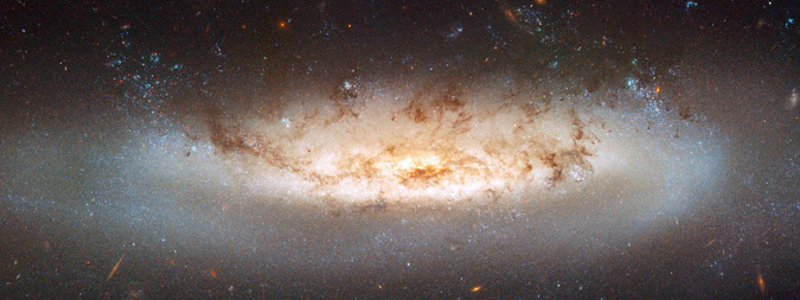
\includegraphics[width=\linewidth]{figures/introduction/rampressure.jpg}
    \caption{An illustration of the ram pressure stripping experienced on a
    galaxy, whose interstellar gas in moved, quenching the star formation since
the ``fuel'' of this process is dropped out.\label{fig:rampressure}}
\end{figure}

The local environment plays also an important role. Several physical processes
are at work inside galaxy groups because of the galaxy over-density relatively
to the background field. They are mainly caused by interactions between each
galaxy and/or the group. Galaxy mergers (essentially major mergers involving
two galaxies of equivalent masses) are expected to morphologically transform
galaxies to spheroidal \citep{Naab+99,Bournaud+05}, and to create star
formation bursts inside merging galaxies \citep{Cox+08,Teyssier+10}. In the
other hand, the dense environment acts too on galaxy properties. Tidal forces
exerted by the group and the ram pressure stripping can remove the outer
gaseous regions in orbiting galaxies leading to a quenching of the star
formation \citep{Larson+80,Bekki+13}.

Some of these intra-group physics were already, more or less well, introduced
in SAM of galaxy formation \citep{Okamoto+03,Lanzoni+05,Font+08,Guo+11}. But
all these methods tend to over-simplify, by use of simple formulas, very
complex processes depending on several parameters and the galaxy environment. A
better modeling of the physics involved in galaxy group should improve the SAM
and correct their difficulties in fully describing the observed Universe. This
can only be achieved with a good definition of the environment for galaxies,
and galaxy groups in redshift space are exactly this definition of environment.

\section{The importance of galaxy groups}
\label{sec:the_importance_of_galaxy_groups}

\subsection{Galaxy group physics}
\label{sub:galaxy_group_physics}

Observed galaxy groups are a direct consequence of this hierarchical growth of
structure. Galaxies therein are affected by this growth since they formed in
dark matter sub-halos that merged with most massive halos along the Universe
expansion according to the hierarchical scenario \citep{Lacey+93}. So their
properties must be correlated with their parent dark matter halo and reflect
their physical processes history inside it. Some evidence of such a modulation
of galaxy properties were already observed previously on the galaxy luminosity
\citep{Robotham+10} and stellar mass \citep{Yang+09} functions, with the galaxy
environment.

Galaxies can be classified in two distinct populations: a blue population of
gas rich and young stellar population and a red one, poor in gas with an old
stellar population \citep{Driver+06}. This bi-modality is also visible in their
morphologies where red galaxies are essentially ellipsoidal and blue galaxies
are spiral. A segregation of these galaxies exists with the environment close
to our epoch (low redshifts): red galaxies lie in dense environment such as
clusters, while the blue population is more present in the field (outside dense
environments as clusters or groups). This is clearly an effect of the
environment, where in clusters, the dense region allows the intra-cluster gas
to be hot enough to stop the star formation of galaxies, leading to an old and
red stellar population. In lower dense region, mergers and various interactions
implying galaxies are frequent and boost the star formation.

But some other properties lead to discrepant results. For example, the star
formation rate (SFR) doesn't show a dependence on the environment according
to~\cite{Peng+10} except for high stellar mass galaxies, but following
\citet{vonderLinden+10}, there is clearly a trend of decline of the SSFR for
star forming galaxies towards groups center (for all galaxy masses). The
results of~\cite{Peng+10} are surprising since in groups and clusters, galaxies
are massive (in stars) due to the cannibalism that contributed in the past to
the formation of the structure. Moreover, the dense environment should quench
the star formation in galaxies due to the intra-cluster gas preventing the
formation of cold clouds, and so varying with the distance to the center of the
group. This contradiction is possibly explained by the selection of a tracer
for the environment in~\cite{Peng+10} that doesn't distinguish between the two
kind of environment: the local one related to the position of the galaxy
relatively to its halo, and the global environment that characterizes the total
mass embedded in the parent halo of the galaxy.
%
\begin{figure}[htb]
    \centering
    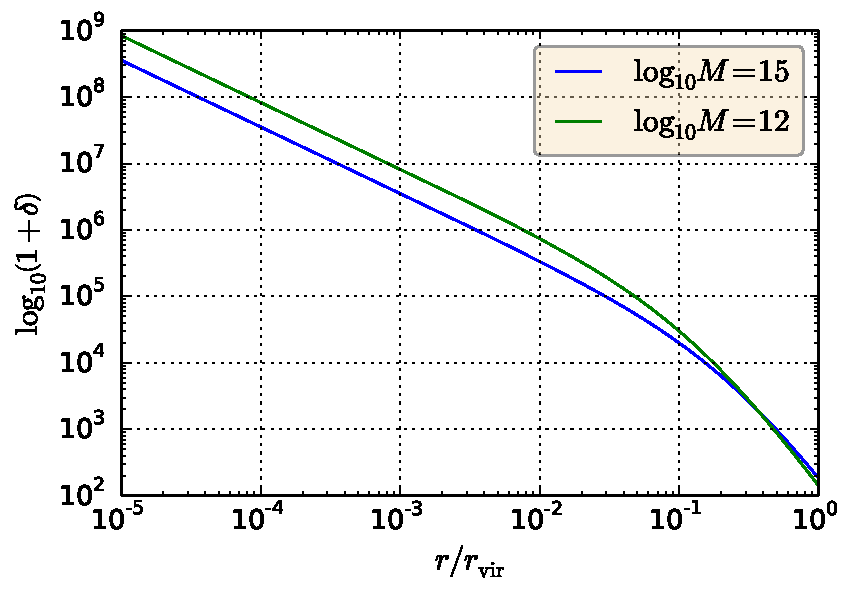
\includegraphics[width=0.6\linewidth]{figures/introduction/overdensity.pdf}
    \caption{The over-density relatively to the mean density for two different
        halos of mass $10^{12}$ and $10^{15} h^{-1} M_\odot$ in function of the
        distance to the halo center in units of virial radius $r_\mathrm{vir}$.
        A density profile from \citet{NFW+97} is assumed with concentrations
    computed from \citet{Maccio+08}.\label{fig:overdensity}}
\end{figure}
%
An example is shown in \bartreffigure{overdensity} where we plot the
over-density as defined in \citet{Peng+10} for two different halo masses with a
density profile from \citet{NFW+97} (see \bartrefappendix{profiles}), a
concentration from \citet{Maccio+08}, in function of the position relatively to
the halo center in units of virial radius. We chose two extremes masses
($10^{12}$ and $10^{15} h^{-1} M_\odot$) to have two very distinct halos. The
over-density is essentially sensitive to the local environment, but the global
one has only a small effect through the concentration parameter. With this
tracer, we can't observe a modulation of the SSFR\@, while the galaxy formation
scenario let us expect an influence of the halo mass with physical processes
regulating the star formation.
%
\remark{%
    Assuming the density profile of \citet{NFW+97}, the over-density $\delta$
    is:
    %
    \begin{equation}
        \delta = \cfrac{\rho \left(r\right) - \rho_m}{\rho_m}
    \end{equation}
    %
    Using equations from \bartrefappendix{profiles}, and writing the mean
    density of the Universe as $\rho_m=\Omega_m \rho_c$ where $\Omega_m$ is the
    density fraction of matter in the Universe (\citet{PlanckXVI} cosmology)
    and $\rho_c$ is the critical density equal to $3 H_0^2/ \left(8\pi
    G\right)$, we finally have:
    %
    \begin{equation}
    \delta = \cfrac{\Delta \overline\rho \left(r/r_\mathrm{vir}\right)}
    {3\Omega_m} - 1
    \end{equation}
    %
    with $\Delta$ the value of the density in units of the critical density
    used to defined a halo relatively to the background, and $\overline\rho$
    the normalized density profile as defined in
    \bartrefappendix{profiles}.
}

\subsection{Galaxy groups as tests}
\label{sub:galaxy_groups_as_tests}

Galaxy groups are not just limited to test and improve the models for the
galaxy formation theory, but also appear in other astrophysical domains. In
cosmology, they are a tool to access the cosmological parameters, such as
the dark energy fraction \citep{Wang+98}. General relativity can be tested
with them \citep{Wojtak+11}.

Unfortunately, a clean characterization of the environment from the redshift
space is difficult since the redshift distortions \citep{Jackson+72}, called
also Fingers-of-God \citep{Tully+78}, caused by the velocity dispersion of the
galaxy group can create overlapping between galaxies of foreground or
background groups. But the over-density used in \citet{Peng+10} is computed
from the nearest neighbors of each galaxies, clearly affected by interlopers
because of projection effects.

\section{Characterizing environment}
\label{sec:characterizing_environment}

\subsection{History}
\label{sub:history}

Many galaxy group catalogs were already published, usually following the first
publications of data from galaxy surveys. First attempts were done with human
selections \citep{Abell+58,Zwicky+61,Rose+76}. The selection was based on non
physical assumptions on galaxy groups, with certain criteria for a visual
over-density of galaxies.

Then the percolation or Friends-of-Friends (FoF) algorithm followed, based on
the knowledge of galaxy physics at this epoch \citep{Huchra+82,Nolthenius+87}.
One of its advantages is that it is based on a physical choice for the way to
link galaxies between them in groups. A linking length is used to relate to
galaxies that are closer than this distance in redshift space. This needs the
use of two different linking lengths in the line-of-sight and perpendicular
directions to avoid the redshift distortions effect. But as argued in
\citet{Duarte+14}, with some priors in the galaxy distribution, these links must
be adjusted to the mass of the group (i.e.\ its richness) to be complete in the
galaxy selection. More recently, \citet{Eke+04} and \citet{Berlind+06}
published too galaxy groups catalogs from the application of the percolation
algorithm, but taking into account, in their selection, the incompleteness
induced by the galaxy surveys used.

\citet{Marinoni+02} developed a method similar to FoF but with the use of a
redshift space partitioned into Voronoi cells, to have an initial seed for the
over-density (Voronoi cells volume trace the galaxy density) around each
galaxy. But this method suffers from the necessity to use it in small surveys
in angle because of the difficulty to create a tessellation of the celestial
sphere directly.

With the increasing advances in the galaxy formation processes, capacities of
numerical computation and predictions of the cosmological simulations, started
to appear Bayesian algorithms that used priors on galaxy groups to improve
their extraction from galaxy surveys. \citet{Yang+05,Yang+07} developed an
iterative method to select galaxy groups based on a density contrast criterion,
which uses assumptions based on cosmological simulation results for the density
profile of groups.

Galaxy surveys have limitations that are difficult to overcome in galaxy group
algorithms. In the case of photometric redshifts surveys, probabilistic
Friends-of-Friends were developed to attempt avoiding the large (and sometimes
catastrophic) uncertainties in redshift measures \citep{Liu+08}. Then,
probability was used to improve the membership of galaxies inside their groups,
as \citet{DominguezRomero+12}, allowing a more flexible way to affect galaxies.

Finally, group finding algorithms continue their insertion of galaxy formation
results, combining it with the advantage of geometrical methods. An example is
\citet{MunozCuartas+12} that used a FoF applied on dark matter halos associated
to galaxies, with the initial assumption that all galaxies are their own halo,
and so the central galaxy mass is a tracer of the density field (the most
massive central galaxies are associated to the most massive halos).

\subsection{And now\ldots?}
\label{sub:and_now}

Actual and next generations of galaxy surveys allow us to probe galaxy groups
in different aspects, each of them with their improvements and limits. Sloan
Digital Sky Survey (SDSS), with its around one million of spectroscoped
galaxies, gives us a good overview of the density field for a large range of
redshifts. But this abundance of precise redshifts as the counterpart that not
all galaxies have spectroscopic redshifts, and around 5--10\% of galaxies,
because of the fiber collision problem \citep{Blanton+03}, need to fall back to
photometric redshifts, more inaccurate. The Galaxy And Mass Assembly, at its
final stage, will contain around $300\;000$ galaxies with a spectroscopic
redshift \citep{Hopkins+13}, less than the SDSS\@. But the completeness of the
sample will be higher than the SDSS with $\simeq99\%$ of the sample
spectroscoped. The counterpart is a less precise measurement of galaxies
recession velocities \citep{Robotham+11,Hopkins+13}. Moreover, the adjoining
angular size is lower because of the fragmentation of the survey regions. But
those galaxy samples are from different sky region allowing to take into
account the cosmic variance in the statistics. In consequence, galaxy group
algorithms must be flexible to be applied and give the same result in many,
different and (surprisingly) creative future galaxy survey projects. Their
common limitations and advantages must be taken into account when developing
it.

So we need to go beyond the usual standard and static definition of groups and
work with the inevitable polluted environment of extracted galaxy groups to
have a precise understanding of the major physical processes at work inside
galaxy groups. We start by an overview of some common grouping algorithms,
their innovations and limitations in \bartrefchapter{galaxy_group_algorithms}.
Since such algorithms must be tested in order to access their capacities in
recovering the clustering from redshift space, we detailed the construction of
a galaxy mock catalogue, difficulties inherent to its creation and biases
introduced voluntary or not inside \bartrefchapter{mock}. We were also
interested in the most popular algorithm that is the Friends-of-Friends or
percolation algorithm and performed a detailed test on its performances in
\bartrefchapter{friends_of_friends_algorithm}. MAGGIE, a probabilistic galaxy
group algorithm that avoids the importance of interlopers in the galaxy group
properties observed is described and analyzed in \bartrefchapter{MAGGIE}. In
\bartrefchapter{sdss}, we described our analysis of the Sloan Digital Sky
Survey in the goal of a future application of MAGGIE on its database.

% vim: set tw=79 :

\chapter{Galaxy group algorithms}
\label{cha:galaxy_group_algorithms}
\minitoc%

As said previously, a good characterization of the galaxy environment implies a
good selection of galaxy groups. But galaxy observations are made in redshift
space, where the velocity dispersion of galaxies inside clusters stretch the
line-of-sight distribution of galaxies. Galaxies in a structure are not seen in
a local region of the space, but the structure is extended in larger range of
redshifts from the projected phase space, which is the only one accessible by
an observer.
\note{Add a citation to article.}
In consequence, the extraction of a galaxy group from the redshift space is
complex because a galaxy in the field can be associated to a group if it
pertains to the range of redshift of the group, and is inside the observational
cone formed by the virial radius. Such a galaxy is called an interloper (inside
the group by selection, but not pertaining to it in reality).
\note{Add the schema of the stage for it.}

A large number of group catalogues were constructed with a large panel of
method for selecting in order to go past the difficulties introduced by the
redshift distortions. A summary of some of such galaxy group algorithm follows,
with a description of their strengths and weaknesses.

\section{Some algorithms}
\label{sec:some_algorithms}

\subsection{\citet{Marinoni+02}}
\label{sub:marinoni02}

\subsubsection{Description}
\label{ssub:description}

This algorithm is a kind of modified version of the Friends-of-Friends
algorithm. The idea is to use over-densities of galaxies in the three
dimensional space (reconstructed simply from the redshift space), and use them
as potential centers for groups. Over-densities are estimated by use of a
Voronoi partition of space. The set of Voronoi cells forms a complete partition
of space, and the volume of a cell is inversely proportional to the galaxy
density around the galaxy in the cell. Then galaxies are sorted by decreasing
densities in order to use them as potential galaxy groups.

\begin{figure}
    \begin{minipage}{0.33\linewidth}
    \centering
    \subfloat[Convex hull]{%
        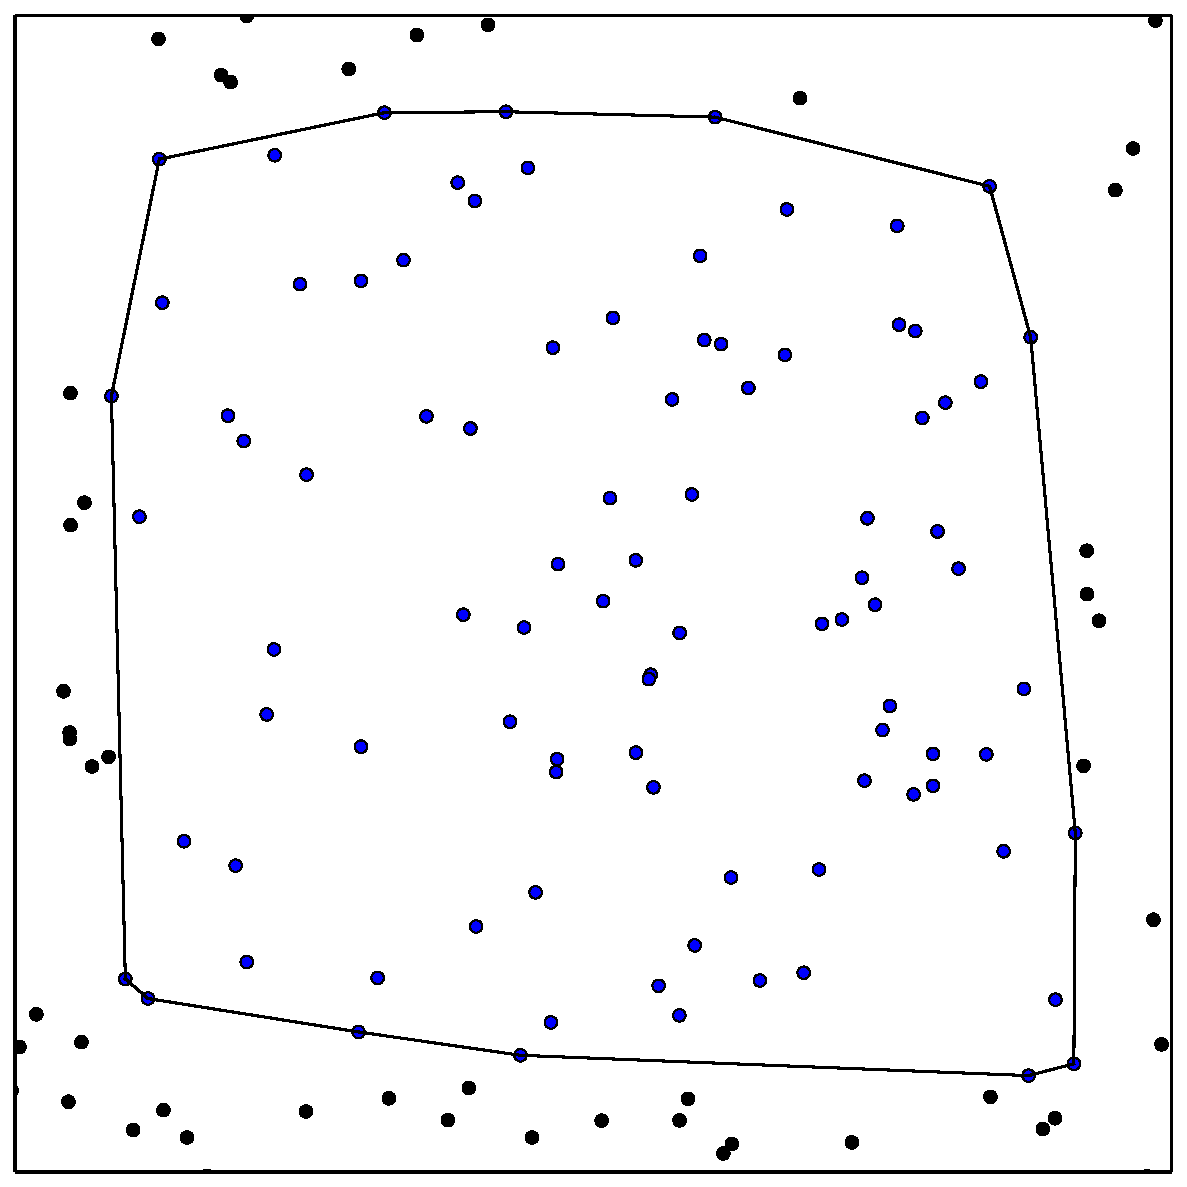
\includegraphics[width=\linewidth]{figures/algorithms/convex_hull.pdf}
    }
    \end{minipage}
    \begin{minipage}{0.33\linewidth}
    \centering
    \subfloat[Delaunay]{%
    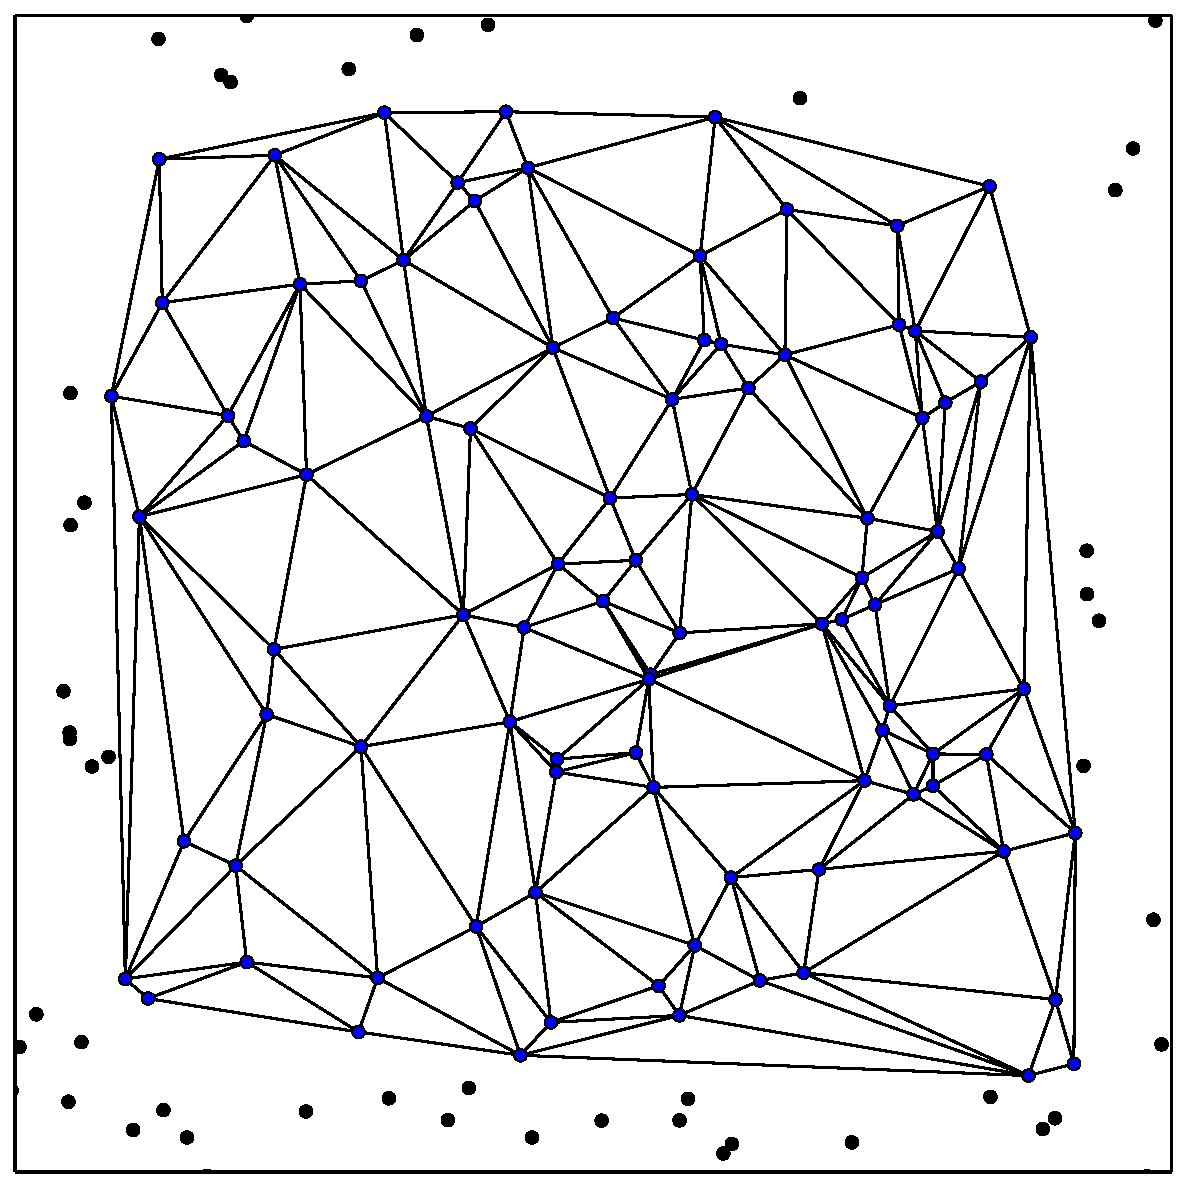
\includegraphics[width=\linewidth]{figures/algorithms/delaunay.pdf}
    }
    \end{minipage}
    \begin{minipage}{0.33\linewidth}
    \centering
    \subfloat[Voronoi]{%
    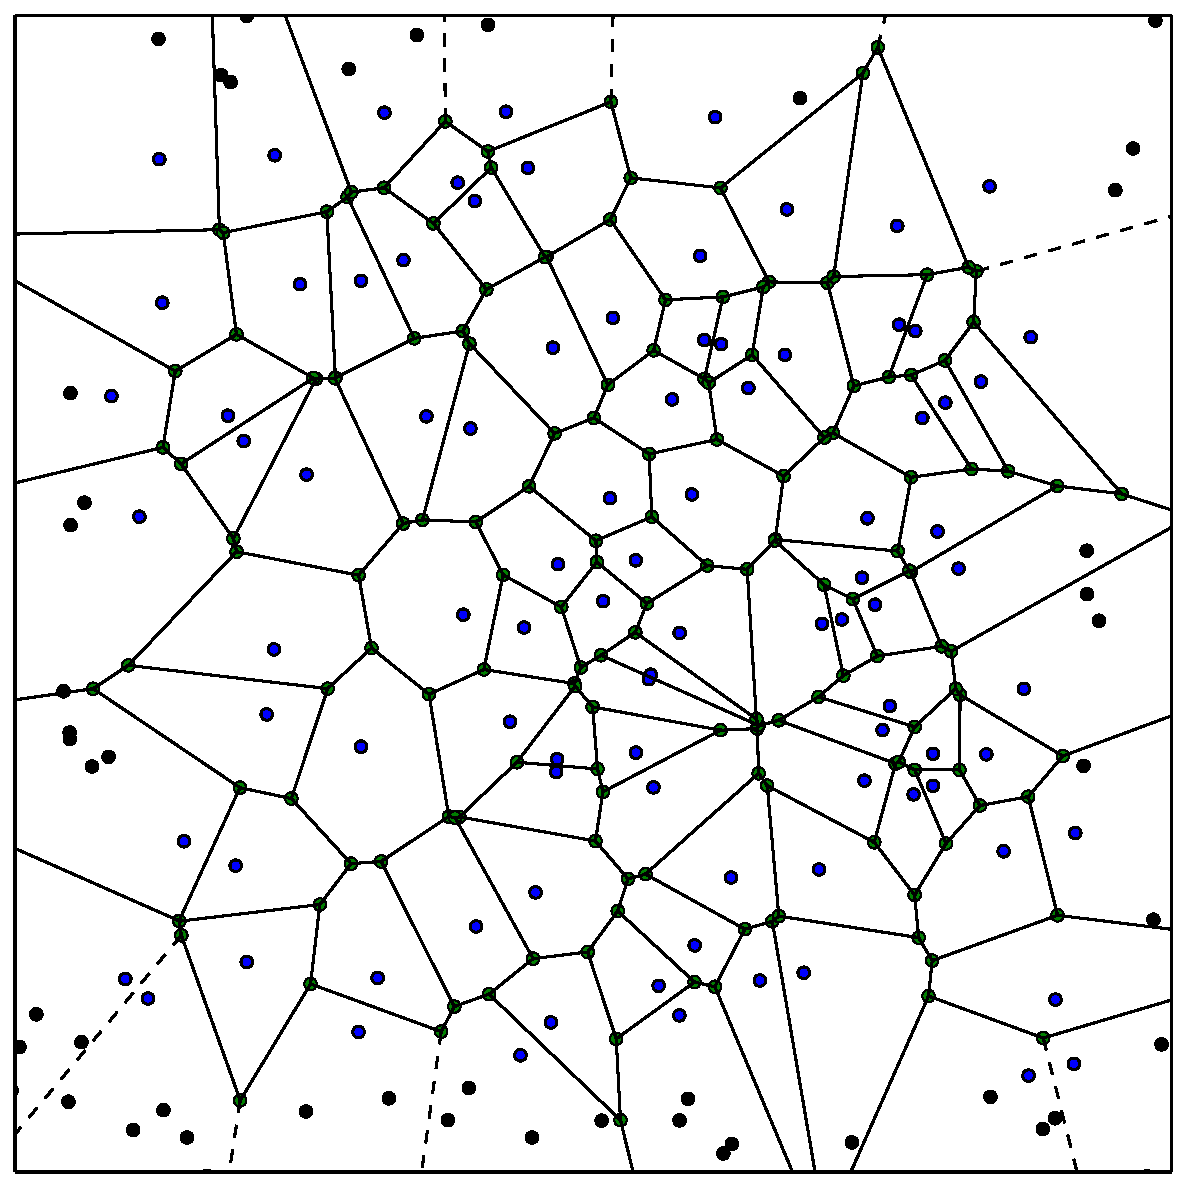
\includegraphics[width=\linewidth]{figures/algorithms/voronoi.pdf}
    }
    \end{minipage}
    \caption{Illustration of the tessellation of the space in a sub-sample of
        randomly positioned points. In \emph{black} the real point distribution
        (reflecting the real galaxy distribution) and in \emph{blue} the
        sub-sample used for the tessellation (reflecting the volume limited
        galaxy survey). (a) The convex hull is the set of points forming the
        hull of the sample. (b) The Delaunay mesh is represented by the lines
        interconnecting points. Each triangle of the mesh has his
        circumscribing circle without a point inside it by definition. (c) The
        Voronoi partition is the dual of the Delaunay mesh. Each node is the
        result of crossing median of the Delaunay mesh. Working on a sub-sample
        of galaxies shows that the Delaunay mesh is not well constrained at
    edges, and the Voronoi cells are affected too. A consequence is that their
volumes are biased and not corresponding to the real galaxy density around
them when too close to borders.\label{fig:convex_delaunay_voronoi}}
\end{figure}

The procedure for selecting galaxy groups is divided in three principal steps,
with an additional phase of initialization. The latter consists on the creation
of the Voronoi-Delaunay tessellation of the galaxy sample in three dimensional
space. For its construction, the idea is to generate a sample of coordinates in
a superior dimension by adding the distance to the origin of each points in it.
Then, the convex hull in this space is computed. It is the set of points
forming the hull of the sample. Projecting the convex hull to the initial space
returns the Delaunay mesh with the links between points. The Voronoi partition
is the dual of the Delaunay mesh and be can deduced from it. An illustration of
each set of points is given in \bartreffigure{convex_delaunay_voronoi}.

The first step is too search for potential groups by using the Voronoi
partition. Voronoi cells have the property that their volume is inversely
proportional to the density of points around each point. In case of galaxies,
this allows to access to local density around them. The detected high densities
in the three dimensional space are used as potential group centers. Galaxies
are sorted by increasing volume of their Voronoi cell, i.e.\ decreasing
density. \emph{First-order} galaxies, first linked to these potential groups,
are searched in a 1 Mpc region, using the Delaunay triangulation to access the
neighborhood of the group. If all first-order galaxies are already assigned to
another group, the two structures are merged.

The second step takes into account the redshift distortions, neglected in the
first step. For this, a cylindrical region is created with a base radius
perpendicular to the line-of-sight, and a height of around 20 Mpc. All galaxies
inside this region not already linked as first-order galaxies are second-order
galaxies. The size of the cylinder is chosen to take into account the redshift
elongation introduced in a typical group.

The third step uses the informations created from the two previous steps, which
are only a selection of potential groups. From the richness of those potential
groups, a relation between the richness and the cylinder lengths is deduced
since the the number of galaxies inside a group and its virial mass are
correlated. This implies that the group sample isn't affected by some
incompleteness, as the luminous one. From a constructed complete sub-sample,
the relation between the richness and the characteristics sizes of the cylinder
are deduced and modeled. Then, the second step is reapplied, the cylindrical
region inferred from the previous relations.

\subsubsection{Advantages and weaknesses}
\label{ssub:advantages}

The group extraction doesn't rely too much on physical assumptions as for the
FoF algorithm, but uses a geometrical approach, based directly on the galaxy
sample at disposition. Moreover, there is no free parameters, since the
cylindrical region is then adjusted, based on a relation between the virial
radius and the group richness. This relation is adjusted in a complete
sub-sample of galaxies to avoid incompleteness corrections, the algorithm
should be robust under different galaxy surveys.

But the Delaunay-Voronoi tessellation has some counterparts. The computation of
the Delaunay mesh is very difficult in non-Euclidean spaces, as the redshift
space, from the point of view of an observer. Moreover, the computation of the
volume of the Voronoi cell is complex too, especially with non-Euclidean
spaces. As a consequence, the computation must be done assuming that the
redshift space is perpendicular and fixed in space (in other words, the
line-of-sight direction at different location on the celestial sphere is the
same). Neglecting the celestial distortions limits the application of the
algorithm to a small portion of the sky of a few degrees of side.

In addition, border effects can't be neglected with the Voronoi partition of
space. Since Voronoi cells form a complete partition, cells at edges of the
galaxy sample have an infinite volume size. Also, the volume of cells close to
borders is biased because the distribution of galaxies is unknown beyond the
sample, and the Delaunay mesh can't be fully constrained to reflect the real
density of galaxies at edges. In other words, the volume of Voronoi cells near
edges doesn't really reflects the local density around galaxies, since the
galaxy distribution is unknown beyond the limit of the sample.

Finally, the tessellation is computed for a flux-limited sample of galaxies,
but the density around galaxies is used to search high mass halos first. Since
the luminous incompleteness is decreasing the observed number of galaxies with
increasing redshift, the effect is that nearby groups are searched first. With
the redshift distortions, the consequences of such bias in the selection aren't
trivial to understand on the resulting group catalogue.

In conclusion, the Voronoi-Delaunay method of \citet{Marinoni+02} can't be
really applied to recent galaxy surveys covering a large area of the sky.

\subsection{\citet{Yang+07}}
\label{sub:yang07}

This algorithm takes into account our knowledge on the large scale structure
extracted from the cosmological simulations to improve the grouping of
galaxies. In particular, an assumption is made on the galaxy density profile
inside halos to follow \citet{NFW+97} to define a parameter used to assign
galaxies to groups. A density contrast parameter is defined as the ratio
between the projected density of galaxies inside an halo and the density of
field galaxies (which are the interlopers). Higher is this ratio, higher the
galaxy is likely to belong to the group. The density of galaxies in the halo is
simply the integration of the distribution function along the line-of-sight,
and for interlopers, its the integration of the mean density of the Universe
along the line-of-sight over the Hubble distance. This results in th following
definition for the density contrast:
%
\begin{equation}
    P_M \left(R, \Delta z\right)=\cfrac{H_0}{c} \cfrac{\Sigma
    \left(R\right)}{\overline{\rho}} p \left(\Delta z\right)
\end{equation}
%
where $H_0$ is the Hubble constant, $c$ the speed of light,
$\Sigma\left(R\right)$ the projected surface density of galaxies at the
projected radius $R$, $\overline{\rho}$ the mean density of the Universe and $p
\left(\Delta z\right)$ is the velocity distribution of galaxies in terms of
redshift differences $\Delta z$ with the group redshift. This definition is
problematic: the density of interlopers is assumed to be constant and the same
for all halos. But as described in \citet{MBM+10}, the density of interlopers
is related to the position in the halo, and their velocity distribution isn't
flat.

Using this density contrast criterion implies to have potential groups on which
to apply it. For this, initially, a FoF algorithm is done on the galaxy sample
but with very small linking lengths. This potential groups are seed whose
membership must be updated using the density contrast, as described below.

For each group, its virial mass is estimated from a relation between the group
luminosity and its mass. Initially, this is a constant ratio, then adjusted on
the group sample itself. From it, the density contrast can be computed for each
galaxy on each group. A galaxy is assigned to a group if $P_M>B$ were $B$ is a
threshold. If this condition is satisfied for multiple groups, it is assigned
to the group with the highest $P_M$.

Then group centers and luminosities are recomputed with the new membership,
iterating over the previous step until a convergence in the membership is
observed.

Once the convergence is reached, the relation between the virial mass and the
luminosities of groups is recomputed by abundance matching between the
distribution of group luminosities obtained from the sample and the expected
distribution of virial masses assuming an halo mass function. Then the previous
iterative process is done again, and this goes until a convergence is reached
for the relation.

The algorithm have some lacks that should be technically and physically
corrected to be good enough in the group extraction. Indeed, some incoherences
are present in the implementation of the grouping algorithm. For example, the
given formula for the computation of the virial radius is done for halos being
over-densities of $\Delta=180$ of the mean density of the Universe, while the
computation of the abundance matching is done with the halo mass function of
\citet{Warren+06} for the FoF mass of halos from the cosmological simulation
used. The difference between the FoF mass and the virial mass is significant
and should be taken into account in the grouping process.

\subsection{\citet{DominguezRomero+12}}
\label{sub:dominguezromero12}

This algorithm is an adaptation of \citet{Yang+07}, based on a better Bayesian
approach, noting that the grouping method of \citet{Yang+07} is simply a
learning algorithm called K-means. Instead of assigning in an hard way galaxies
to groups in the iterative process, this method assigns responsibilities,
equivalents of a probability of belonging to a group, pondered over all groups
in the sample, using the density contrast definition above as some probability
to be in the group.

First, potential groups are estimated assuming that the most luminous galaxies
are linked to most massive systems. Then, galaxies are assigned to a group as
satellites members if they have a density contrast superior to a chosen low
threshold to allow a maximum of galaxies to belong to the group, without
introducing too much interlopers since their responsibilities will be low and
won't affect group properties. As for \citet{Yang+07}, an iteration over the
membership and the relation used to compute virial properties is done until
convergence. Finally, galaxies are hardly assigned to a group, the one for
which the responsibility is the highest.

Inconvenient of this method are essentially inherited from \citet{Yang+07}.

\subsection{\citet{MunozCuartas+12}}
\label{sub:munozcuartas12}

This method is similar to the FoF algorithm, but applied directly on halos and
not on galaxies. From an initial set of halos, a maximal circular radius is
computed from the virial radius in the transverse direction to the
line-of-sight. A maximal length of search for the redshift dimension is
estimated from the circular velocity of the halo. Those halos are sorted by
decreasing masses. For each one, other halos (and their galaxies) are merged
into the current halo if they belong to the ellipsoid defined by the two
lengths defined above, centered on the halo.

Then, group properties are computed from the membership obtained previously.
The new virial masses are evaluated with an abundance matching between the
group stellar masses and the halo mass function. The iteration is stopped once
the number of halos doesn't change.

This method doesn't have any free parameter and doesn't rely on too much
assumptions and models. Only the abundance matching can be responsible for a
bias, since the virial mass is crucial in the merging of halos. As mentioned by
\citet{Yang+07}, the one-to-one assumption of the abundance matching creates an
intrinsic dispersion in the mass estimation that is relatively low, and thus
should not affect the galaxy grouping.

\section{Discussion}
\label{sec:gga_discussion}

We can extract common principles of the different algorithms we described
above. There are two approaches for the galaxy grouping: a geometrical one
based only on the positional informations of galaxies and a Bayesian one using
priors on group properties and galaxies therein. What emerged is that a large
majority of these algorithms make a harmonious combination of these approaches
in order to conserve only their strengths. A typical geometrical algorithm is
the Friends-of-Friends (see \bartrefchapter{friends_of_friends_algorithm}),
linking galaxies between them if they are closer than a linking length. This
method has the default of creating bridges between two different galaxy groups
if two of their members are closer than the linking length. Adding priors to
such a scheme, the membership can be improved by breaking the problematic
bridges. This is a good summary for the method of \citet{Marinoni+02} or
\citet{MunozCuartas+12}. Moreover, the bias in distance introduced by redshift
can be reduced with same prescriptions ad done in \citet{Liu+08}.

\begin{figure}[htb]
    \centering
    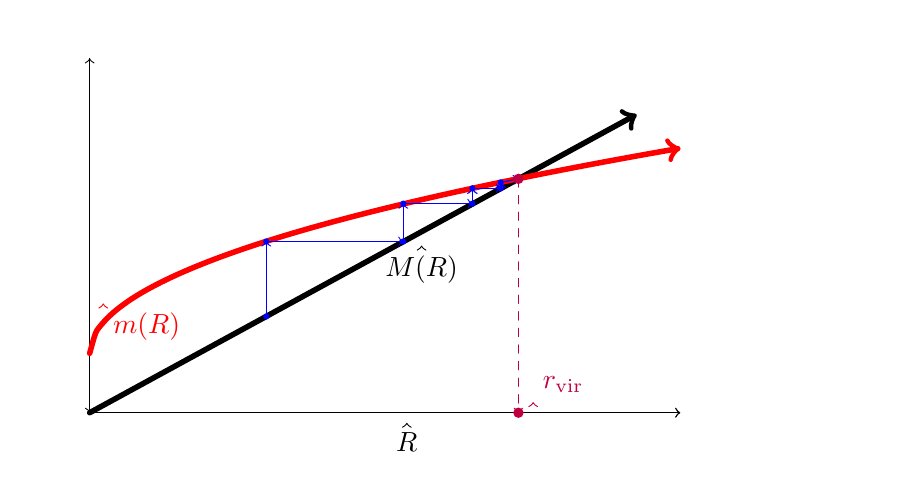
\begin{tikzpicture}[line cap=round,line join=round,->=triangle 45,x=1.0cm,y=1.0cm,scale=0.75]
        \clip(-1.05,-1.06) rectangle (13.19,6.52);
        \draw (0,6)-- (0,0);
        \draw (0,0)-- (10,0);
        \draw [line width=2pt,color=black] (0,0)-- (9.26,5.05);
        \draw [->] (0,0) -- (10,0);
        \draw [->] (0,0) -- (0,6);
        \draw[line width=2pt,color=red, smooth,samples=100,domain=0.00001:10.0] plot (\x, {1.1*\x^(0.5)+1}) ;
        \draw [->,color=blue] (2.99,1.63) -- (2.99,2.9);
        \draw [->,color=blue] (2.99,2.9) -- (5.31,2.9);
        \draw [->,color=blue] (5.31,2.9) -- (5.31,3.54);
        \draw [->,color=blue] (5.31,3.54) -- (6.48,3.54);
        \draw [line width=0.5pt,color=blue] (6.48,3.54) -- (6.48,3.8);
        \draw [->,color=blue] (6.48,3.8) -- (6.96,3.8);
        \draw [line width=0.5pt,color=blue] (6.96,3.8) -- (6.96,3.9);
        \draw [->,color=blue] (6.96,3.9) -- (7.26,3.96);
        \draw [dash pattern=on 3pt off 3pt,color=purple] (7.26,3.96)-- (7.26,0);
        \draw[color=black] (5.62,2.83) node[below] {$M(R)$};
        \draw[color=black] (5.37,-0.17) node[below] {$R$};
        \draw[color=red] (0.23,1.85) node[below right] {$m(R)$};
        \fill [color=blue] (2.99,1.63) circle (1.5pt);
        \fill [color=blue] (2.99,2.9) circle (1.5pt);
        \fill [color=blue] (5.31,2.9) circle (1.5pt);
        \fill [color=blue] (5.31,3.54) circle (1.5pt);
        \fill [color=blue] (6.48,3.54) circle (1.5pt);
        \fill [color=blue] (6.48,3.8) circle (1.5pt);
        \fill [color=blue] (6.96,3.8) circle (1.5pt);
        \fill [color=blue] (6.96,3.9) circle (1.5pt);
        \fill [color=purple] (7.26,3.96) circle (2.5pt);
        \fill [color=purple] (7.26,0) circle (2.5pt);
        \draw[color=purple] (7.51,0.18) node[above right] {$r_{\mathrm{vir}}$};
    \end{tikzpicture}
    \caption{Graph illustrating the convergence of the group membership by
    iterations.\label{fig:convergence}}
\end{figure}

Iteration seems to be a key in a good grouping algorithm. A convergence in the
galaxy membership is assured by updating group properties along iterations, and
using it to constrain the selection. The convergence in various scaling
relations in groups is also assured by iterations, giving a self-consistency of
the clustering with the data itself: galaxy group algorithms are special kind
of machine learning algorithm. For example, we suppose an algorithm using a
relation between the stellar mass of groups and its virial mass (see
\bartreffigure{convergence}). The stellar mass of the group in red increases
with the projected radius since the number of galaxies inside it increases.
There is also a relation between projected radius and virial mass. Starting
with an initial guess for the virial mass, we can perform a galaxy selection
and estimate a stellar mass for the group. With the relation, we can make a new
estimation of the virial mass. This process goes until the convergence
represented by the virial radius $r_\mathrm{vir}$ in
\bartreffigure{convergence}.

The Bayesian approach used in the described galaxy group algorithms as also its
counterparts: if the chosen models are bad, the clustering will be affected
too. For example, \citet{Yang+05} assumes a flat line-of-sight velocity
dispersion and a flat distribution of interlopers in the computation of density
contrast, which clearly depends on the projected radius pointed by the
observer. Another problem is the way to test such algorithms. Previously
described algorithms were tested on different galaxy mock catalogues, not
constructed in the same way, without the same physics applied inside them. In
consequence the comparison is very difficult because not operated in the same
conditions. And the definition of an optimal extraction, and the statistics
used assess their perfomances differ with galaxy group algorithm developers.

To go beyond such limitations that will never be completely avoided,
a probabilistic approach of galaxy groups seems to be a good compromised (see
\bartrefchapter{MAGGIE}). Moreover, the tests for algorithms must be well
defined, with a common galaxy mock catalogue to perform the comparisons and a
good definition of the statistics to use. How well are recovered galaxy groups?
How well they are polluted by interlopers? How many selected groups are
spurious? How virial properties of the parent halo are recovered? How scaling
relations are recovered? They are the questions to answer in order to
characterize the quality of a grouping algorithm.

% vim: set tw=79 :

\bartchapterimage{simudm}
\chapter{Generate mock catalogues}
\label{cha:mock}
\bartthumb{thumb_simudm}
%
\section{Introduction}
%
A mock catalogue is a useful tool to test algorithms involving galaxies in
order to see if it is operational in a realistic situation. Many of the
properties of galaxy surveys can be simulated: the spatial clustering of
galaxies, luminosity function, incompleteness and measures errors are some
examples of them. There are different methods to obtain such a mock catalogue.
All of them involves cosmological simulations and there halos of dark matter.
According to the model of galaxy formation, we can use halo occupation
distribution (HOD) to populate dark matter haloes with galaxies and putting
some luminosity functions (for example) as constraints. We can follow galaxies
in semi-analytical models (SAM) in those cosmological simulations outputs in
order to have statistical properties of galaxies which agree with observational
results. With such realistic galaxies, we can use those simulation boxes to
place an observer into it, and create a mock survey. But to have a realistic
mock catalogue, it's necessary to take care of many things which will be
described in the next section.
%
\section{Mock structure}
%
In all this section, we will assume that we have already in our possession a
dark matter simulation box which has been populated with galaxies with one of
the methods described below (SAM, HOD\ldots). At this step, physical properties
of those galaxies aren't interesting.
%
\subsection{Placing boxes}
%
The first step to make a mock catalogue is to get galaxies positions like in a
survey, to get an $(\alpha,\delta)$ frame to simulate the sky coverage of
survey and, at the same time, project galaxies on the sky, masking to us some
spatial modulations of galaxy properties.

We want that a false observer see the same volume extension of a true survey.
For example for the SDSS survey, we can measure redshift to a value of 0.3 (and
more!). But the problem is that the majority of the simulation boxes have a
size of around $L_{\mathrm{box}}=100-300 h^{-1}$ Mpc, letting us with a maximal
redshift in our false survey of around ${H_0}{L_{\mathrm{box}}}/c\approx 0.025$
in the case of a box of $100 h^{-1}$ Mpc sized. Bigger simulations exist, and
maybe can allow us to access to bigger redshifts, but this increasing size
reduces the resolution of the simulation in particle mass and therefore we
can't have low mass halos in the simulations.

The solution is to take a ``little'' simulation box and to replicate it and to
make some bigger ``Tetris'' cube until we reach the maximal redshift we want.
An example of the resulting ``mock cube'' is shown on figure
(\ref{fig:cubemock}).
%
\begin{figure}
    \centering
    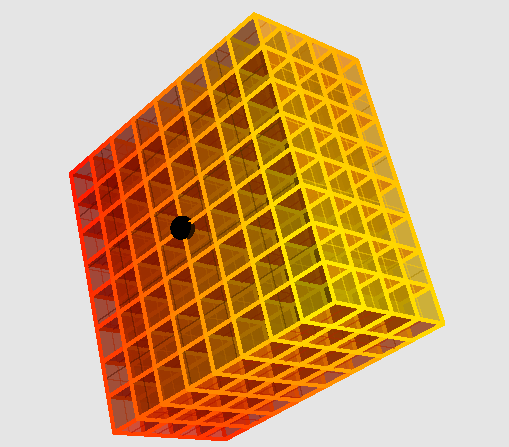
\includegraphics[width=0.5\linewidth]{figures/mock/mock}
    \caption{The structure of the mock catalog once we have replicated the
        simulation box chosen to populate dark matter halos. Each cube
        represents a simulation box whose galaxies where randomly
        transformed in their positions. Placing an observer at a given
        position, we can access different geometry for the survey and go to
    higher redshift ranges.\label{fig:cubemock}}%
\end{figure}

Now if we take an observer at some position into this big box, we can have
different sky coverage for the observer. The simplest is to place the observer
at a corner, which gives a solid angle of $\pi/2$ steradians. At the centre,
we have a full sky coverage but we reduce the redshift extension by 2.

If we want to care about redshift evolution of galaxies for the observer, we
need to use other snapshots at different redshifts. Box sizes are similar in
comoving coordinates, and different in physical coordinates due to the
variation of the Hubble constant with redshift ($h$ depends en $z$). But we
can simply join cubes in comoving coordinates, facilitating the computation
of the mock catalogue. Indeed, the cosmological redshift of the galaxy, only
consequence of the Hubble flow, can be solved from the relation between the
redshift and the comoving distance, equals to the comoving transverse
distance (or proper motion distance) in the case of a flat Universe
($\Omega_k=0$). Moreover, the comoving separation $R$ between two points
with angular separation $\theta$ on the sky, at comoving distance $D_c$ from
the observer, are simply related by a geometrical relation $R=\theta D_c$.
This separation $\theta$ deduced from comoving coordinates should be the
same as those of the observer if he knows perfectly the cosmological
redshift of galaxies. The observer wants to know the physical separation
$R_p$ between the two galaxies, so $R_p=\theta d_\mathrm{ang}$ giving
$R_p \left(1+z\right)= R_p/a\left(t\right)=R_c=\theta D_c$.
%

Placing boxes as described previously can creates a perspective effect from the
point of view of an observer, and the consequences aren't predictable in a
statistical sense when we try to use the mock catalog. To avoid this, we apply
some transformations on galaxies in the initial cube like inversions, rotations
and periodic translations. Rotations are multiples of $\pi/2$ around the three
principal coordinates axes, because if other rotations are allowed, this can
create some over-densities in some regions of the final mock which aren't
physical. Translations are performed on the three principal axes
and when galaxies are out of the initial cube, periodic conditions are applied.
All of those transformations are randomly generated for each cube in the final
mock catalogue.
%
\subsection{Physics}
%
\subsubsection{Celestial coordinates}
%
The first step to simulate this is to transform Cartesian coordinates in the
3D space to celestial coordinates ($(\alpha,\delta)$ frame). Getting these
coordinates is the same as computing spherical coordinates.
%
\begin{equation}
    \alpha=\left\{ \begin{array}{lcr}
     \mbox{arctan2}(Y,X)+2\pi & \mbox{if} & Y>0 \\
     \mbox{arctan2}(Y,X) & \mbox{else} & \\
    \end{array}\right.\nonumber%
\end{equation}
%
\begin{equation}
    \delta=\mbox{sign}(Z)\arccos\left(\frac{\sqrt{X^2+Y^2}}{\sqrt{X^2+Y^2+Z^2}}\right)
\end{equation}
%
\subsubsection{Redshifts}
%
In our case, the origin of coordinates is the observer. If we keep the distance
as calculated previously, the observer can still have precise determination of
the distance of a galaxy. In reality, we observe it in redshift space so the
redshift as distance indicator is biased by peculiar velocities. Our initial
galaxy catalog allow us to get the velocity of a galaxy, so we can compute the
line of sight (los) velocity of this galaxy relatively to the observer.
%
\begin{equation}
    v_{\mathrm{los}}=\cfrac{\vec{OG}.\vec{v_{\mathrm{pec}}}}{||\vec{OG}||}
\end{equation}
%
where $O$ is the observer and $G$ the galaxy, $\vec{v_{\mathrm{pec}}}$ its
peculiar velocity. This velocity has a sign. The redshift is just the
expression a shift in wavelength due to a velocity. The observed wavelength
$\lambda$ is linked to the original (emitted) wavelength $\lambda_0$ by:
%
\begin{equation}
    \lambda=(1+z)\lambda_0
\end{equation}
%
The shift caused by Universe expansion is
$\lambda_{\cos}=(1+z_{\cos})\lambda_0$ where the subscript $\cos$ refer to
the cosmological expansion. The shift caused by the peculiar velocity is
$\lambda=(1+z_{\mathrm{pec}})\lambda_{\cos}$. So the observed wavelength is
$\lambda=(1+z_{\mathrm{pec}})(1+z_{\cos})\lambda_0$. The resulting observed
redshift is just:
%
\begin{equation}
    (1+z)=(1+z_{\mathrm{pec}})(1+z_{\cos})
\end{equation}
%
The peculiar redshift is the just due to the relativist Doppler effect:
%
\begin{equation}
    (1+z_{\mathrm{pec}})=\sqrt{\cfrac{1+\beta}{1-\beta}}
\end{equation}
%
with $\beta={v_{\mathrm{los}}}/{c}$. The cosmological redshift is
approximated by $z_{\cos}={H_0}{D}/c$ where $D$ is the physical distance of
the galaxy to the observer and $H_0$ the Hubble constant.
%
\comments{I think we need to add the velocity of the Local Group in the
redshift, because in our case the observer has a null velocity. Maybe
corrected in SDSS data?}
%
Applying this method to mock catalogue, we can have galaxies whose distance
is biased by peculiar velocities in redshift space. With such a treatment,
the velocity dispersion of galaxies in groups leads to the apparition of
``fingers of God'' as seen in observations in redshift space.
%
\subsubsection{Survey mask}
%
With our frame in redshift space relative to the observer, we can apply
different masks on angular coordinates according to the survey we want to
mimic. An example of such a mask is in appendix (\ref{ap:sdss}).
%
\subsubsection{K-corrections}
%
In reality, an observer study galaxies in a given bandwidth in wavelength and
can't use the bolometric flux of the object. With the expanding Universe, all
the spectral energy distribution (SED) of galaxy is shifted. All wavelengths
are shifted by the same value for a given redshift. So, knowing the luminosity
$L$ of a galaxy in a given band in reality (using the true SED), computing its
apparent magnitude for an observer isn't as easy as correcting for the distance
modulus. The observer in the same band sees a different part of the true SED\@.
The flux observed in the same band as the true flux is maybe higher or lower. A
correction for this effect is needed and must be taken into account in our mock
catalogue.

As explained before, this correction depends on the SED of galaxies and the
band used in the survey. The common way of correcting, it when we have a
multi-band photometry, is to fit the observed SED in those bands with
theoretical templates of SEDs. Such templates can be obtained with existing
programs as PEGASE \comments{Add references}, which give us SEDs with some
assumptions on the galaxy. But those programs are a little time consuming,
which can be a problem for mock when we want to run several of them. A good
solution is provided by \citet{Chilingarian+10}, where the K-correction is
fitted on templates for SED as given by PEGASE in terms of a polynomial of the
redshift of the galaxy and its colour. The corresponding K-correction is
precise for redshifts until 0.3 in different survey bands (including $ugriz$
for the SDSS). This work reduces the computation of K-corrections to the use of
simple polynomial relations and make our task easier.

By definition, the K-correction $K$ for a galaxy of apparent magnitude $m_X$
in a given band $X$ and absolute magnitude $M_X$ in the same band is:
%
\begin{equation}
    {m_X}={M_X} + {5\log_{10}\left({d_{\mathrm{lum}}\left[pc\right]}\right)} - 5 + K
\end{equation}
%
In our case, the K-correction depends on the redshift of the galaxy and its
colour in apparent magnitude given two bands. So we can rewrite:
%
\begin{equation}\label{eq:appmag}
    m_X = M_X + 5\log_{10}\left({d_{\mathrm{lum}}\left[pc\right]}\right) - 5 + K( z, m_X - m_{X'} )
\end{equation}
%
where:
%
\begin{equation}
    K(z,m_{X}-{m}_{X'})=\sum_{i=0}^{N_i}\sum_{j=0}^{N_j}{a_{ij}}{z^i}{{(m_X-{m}_{X'})}^j}
\end{equation}
%
and $a_{ij}$ is a ${N_i}\times{N_j}$ matrix containing the coefficients of the
two dimensional polynomial. These coefficients depend on the bands of the
survey used for the colour computation.

The observer in the mock can just, in theory, access to apparent magnitude
of the survey. But we don't know in advance these magnitudes, and as we can
see in the expression of equation (\ref{eq:appmag}), we need apparent
magnitudes to compute apparent magnitudes. If we use the other bands of the
survey, with $a_{ij}$ coefficients, we can always write a set of equations
for a galaxy which involves all apparent magnitudes of the survey. So we can
write a set of non linear equations with polynomial of order $N_j$ (redshift
of the galaxy is supposed to be known). Numerically it's easy to solve this
set of equations, and relatively fast with equations solvers or by
iterations. In practice, the first is faster than the second method, even if
both methods give similar results in apparent magnitudes.
%
\subsubsection{Flux limit}
%
We have seen in appendix (\ref{ap:sdss}) that spectroscoped galaxies are just
defined for galaxies whose apparent magnitude is less than 17.77 in $r$
band. So, in all the redshift sample, we miss some galaxies not sufficiently
bright. To take into account this effect, we remove galaxies not reaching
the limit apparent magnitude of the survey.
\comments{Some surveys have variation of this flux limit with the sky
position. Maybe something like this to check for SDSS?}
%
\subsubsection{Spectroscopic and photometric redshifts}
%
Sometimes, we can't access to spectroscopic redshifts which are more precise
than photometric redshifts. In the SDSS, for example, this is due to tiling
process. Fibers analysing the spectrum of galaxies can't be closer from each
other than 55'', so if for a target galaxy (selected to get a spectrum)
there is an other galaxy closer than those 55'', the tile containing all fibers
doesn't have the possibility to measure the redshift of this galaxy. This
problem is more significant for dense regions in the celestial plane. A very
good algorithm to placing tiles in order to limit the number of missed galaxies
(\textit{ie} the number of fiber collision) has been applied in the galaxy
sample of the SDSS\@.
%
\note{Cite Blanton or Lupton!}.
%
But there is still some galaxies without spectroscoped
redshifts. If we remove those galaxies from our sample, there will be a
spectroscopic incompleteness with unknown effects on our results.
%
\note{Say something on how to correct}
%
\subsubsection{Observational errors}
%
\note{Errors exist in redshift measurement, photometry, astrometry\ldots We
add them in our mock catalogue by simply assuming a distribution for errors
around the true value, and then applying it to the galaxy in our mock
catalogue.}
%
\comments{Think in a way of adding the surface brightness selection
criterion on the mock catalogue. It will be great!}.

\begin{table}
\caption{Doubly complete mock galaxy subsamples\label{tab:samples}}
\begin{center}
\setlength{\tabcolsep}{3pt}
\begin{tabular}{lccccccc}
\toprule
\toprule
ID & $M_r^{\max}$ & $L_r^{\min}/L*$ & $z_{ \max }$ & Number & $n$
& $n^{-1/3}$ & Fraction\\
          &            &     &                 &        & ($\rm  Mpc^{-3}$)
& (Mpc) & split\\
\toprule
1 & --18.5 & 0.09 & 0.042 & \ \,47158 & 0.0125 & 4.32 & 5.3\%\\
2 & --19.0 & 0.14 & 0.053 & \ \,72510 & 0.0099 & 4.66 & 6.1\%\\
3 & --19.5 & 0.22 & 0.066 & 112629    & 0.0078 & 5.05 & 6.6\%\\
4 & --20.0 & 0.36 & 0.082 & 166899    & 0.0058 & 5.56 & 7.4\%\\
5 & --20.5 & 0.56 & 0.102 & 213546    & 0.0040 & 6.29 & 8.6\%\\
6 & --21.0 & 0.90 & 0.126 & 245821    & 0.0025 & 7.40 & 9.9\%\\
\bottomrule
\end{tabular}
\end{center}
\parbox{\hsize}{Notes: Columns are: sample, maximum $r$-band absolute
  magnitude, minimum luminosity in units of $L*$
(adopting $M*=-20.44 + 5\,\log h$ in the SDSS $r$ band from \citealp{Blanton+03}),
maximum redshift,
sample size,
mean density $n$, proxy for the mean separation to the closest neighbor,
$n^{-1/3}$, and the percentage of true groups that are flagged because they are
split during the simulation box transformations.
The minimum redshift of each subsample is $z=0.01$.
}
\end{table}

% personal commands and shortcuts
\def\bpar{$b_\parallel$}
\def\bperp{$b_\bot$}

\bartchapterimage{heic1006a.jpg}
\chapter{Friends-of-Friends algorithm}
\label{cha:friends_of_friends_algorithm}
\bartthumb{heic1006a.png}
\minitoc%

\section{Introduction}
\label{sec:fof_introduction}

Although a lot of galaxy group algorithm are born recently, using our knowledge
on the galaxy formation and evolution processes (as described in the
\bartrefchapter{galaxy_group_algorithms}), for a long time, the
Friends-of-Friends algorithm (hereafter FoF) has dominated. Many catalogs of
galaxy groups have been constructed from redshift space
catalogs,\footnote{\cite{TG76} applied a grouping algorithm in projected space
that turned out to be a Friends-of-Friends algorithm.} using FoF algorithms
(\citealp*{HG82,NW87,RGH89,TrasartiBattistoni98,MZ02};
\citealp{Eke+04,Berlind+06,Tago+10,Robotham+11,Tempel+14}).

Starting with~\cite{NW87},  nearly all FoF group analyses on redshift space
catalogs were accompanied with tests on mock galaxy catalogs derived from
N-body simulations. However, not all FoF developers have applied the same tests
to calibrate their linking lengths.~\cite{NW87} were the first to compute the
accuracy of group masses, as well as radii and velocity dispersions, crossing
times and mass-to-light ratios.~\cite{RGH89} were the first to test the
recovered group multiplicity function.~\cite{Frederic95a} was the first to
measure the galaxy reliability of extracted groups (comparing the FoFs of
\citealp{HG82} and \citealp{NW87}), as later done by~\cite{MZ02}, who also
measured group completeness (against mergers of true groups) and reliability
(against fragmentation of true groups). \citet{Eke+04} also tested the true
group completeness and fragmentation, as well as the accuracy on group sizes
and velocity dispersions. They also considered a quality criterion that amounts
to a combination of galaxy completeness and reliability. Finally,
\citet{Berlind+06} performed similar tests as \citeauthor{Eke+04}, with another
test combining galaxy completeness and reliability. \citeauthor{Berlind+06}
noted that one cannot simultaneously optimize the accuracies on group sizes,
velocity dispersions and [multiplicity function OR combined galaxy
completeness/reliability].

Unfortunately, none of these studies is fully convincing: many did not perform
the full suite of important tests, which we believe are true group
fragmentation (group reliability) and merging (group completeness),  galaxy
completeness and reliability studied separately, and mass accuracy. Many have
not measured the qualities of their LLs in terms of group parameters such as
estimated mass and richness. Few studies have \emph{optimized} the LLs:
\cite{Eke+04} separately optimized \bperp{} and \bpar.~\cite{Berlind+06}
jointly optimized \bperp{} and \bpar{} on a grid, for groups of 10 or more
galaxies, while~\cite{Robotham+11} jointly fit the LLs and their variation with
density contrast and galaxy luminosity for groups of 5 or more galaxies to
optimize for the product of four fairly complex measures of group and galaxy
completeness and reliability. However, there is no strong agreement between the
optimized LLs of \citeauthor{Eke+04}, \citeauthor{Berlind+06}, and
\citeauthor{Robotham+11} (see Table~\ref{tab:groupalgos}).
%
\begin{table}
\caption{Friends-of-Friends linking lengths and physical
parameters\label{tab:groupalgos}}
\begin{center}
\setlength{\tabcolsep}{2.5pt}
\begin{tabular}{llllcrl}
\toprule%
\toprule%
Authors & sample & \multicolumn{1}{c}{$b_\perp$} & \multicolumn{1}{c}{$b_\parallel$} &
\multicolumn{1}{c}{$b_\parallel/b_\perp$} & $\delta n/
n$ & \multicolumn{1}{c}{$\kappa$} \\
\toprule%
Huchra \& Geller 82     & CfA     & 0.23  & 1.34  & \ \ \ \ 6.3  & 20    & 5.7 \\
Ramella et al. 89       & CfA2    & 0.14  & 1.9   & 13   & 80    & 5.8 \\
Trasarti-Battistoni 98  & PPS2    & 0.13  & 1.7   & 13   & 108   & 4.9\\
Merchan \& Zand'z 02    & 2dFGRS  & 0.14  & 1.4   & 10   & 80    & 4.4 \\
Eke et al. 04           & 2dFGRS  & 0.13  & 1.43  & 11   & 178   & 3.9\\
Berlind et al. 06       & SDSS    & 0.14  & 0.75  & \ \ \ \ 5.4  & 86    & 2.3 \\
Tago et al. 10          & SDSS    & 0.075  & 0.75  & 10   & 565  & 1.7\\
Robotham et al. 11      & GAMA    & 0.060  & 1.08  & 18   & 1100  & 2.2\\
Tempel et al. 14 ($M_r<-19$)        & SDSS    & 0.11  & 1.1 & 10 & 178 & 3.0 \\
Tempel et al. 14 ($M_r<-21$)        & SDSS    & 0.066  & 0.67 & 10 & 830 & 1.4
\\
\bottomrule%
\end{tabular}
\end{center}
\parbox{\hsize}{%
\footnotesize Notes: The (normalized) linking lengths
of~\cite{HG82},~\cite{RGH89}, and~\cite{TrasartiBattistoni98} are derived
(using \bartrefequation{bperpdef} and \bartrefequation{bpardef}) from their
physical linking lengths at the fiducial distance and from the mean density at
that distance, as derived by integrating the respective luminosity functions
given by these authors. The linking lengths of~\cite{MZ02} are estimated
directly from the overdensity $\delta n/n$ given by these authors (using
\bartrefequation{dnovernfromb}), those of~\cite{Tago+10} are found from the
densities deduced from the numbers of galaxies counted by these authors (again
with \bartrefequation{bperpdef} and \bartrefequation{bpardef}).~\cite{Eke+04}
provide $b_\perp$ and $b_\parallel/b_\perp$, while~\cite{Berlind+06}
and~\cite{Tempel+14} provide $b_\perp$ and $b_\parallel$. When not provided by
the authors, the overdensity $\delta n/n$ is obtained through
\bartrefequation{dnovernfromb}, and should be multiplied by 1.5 for a more
accurate estimation (see text). Finally, the number of group velocity
dispersions along the LOS, $\kappa$ is obtained with
\bartrefequation{kappafromlls} assuming $\Omega_{\rm m}=0.3$.
}
\end{table}

Moreover, we believe that in this era of large  redshift surveys of $>10^5$
galaxies, it makes little sense to extract groups from flux-limited galaxy
samples, for which most current implementations of the FoF algorithm scale the
maximum separations proportionally to the mean  separation between neighboring
field galaxies, $n^{-1/3}$. Indeed, since the minimum luminosity in
flux-limited samples increases with redshift,  the mean number density of
galaxies decreases with redshift, and thus the mean separation between
neighboring galaxies increases with redshift. Therefore, the standard
implementation of the FoF algorithm leads to groups that become increasingly
sparse and with increasingly higher velocity dispersion with redshift (while
their multiplicity function is preserved). Alternatively, since the mean
neighbor galaxy separation increases with redshift in flux-limited samples,
using a fixed physical linking length leads to lower reliability at low
redshift and lower completeness at higher redshifts. Moreover, grouping
algorithms on flux-limited samples must evaluate the luminosity incompleteness
as a function of redshift, which is difficult and imprecise (e.g.,
\citealp{MDNC02,Yang+07}). It is therefore much safer to consider subsamples
that are complete in both distance and galaxy luminosity (as done for FoF
grouping by \citealp{Berlind+06}, \citealp{Tago+10} and \citealp{Tempel+14}).
Admittedly, one recovers at best of order of one-quarter of the galaxies of the
flux-limited sample, but one then avoids extracting a heterogeneous sample of
groups (see \citealp{Tempel+14}) whose sizes and velocity dispersions stretch
with redshift (when scaling the physical linking lengths with $n^{-1/3}$) or
whose completeness and reliability vary with redshift (when adopting fixed
physical linking lengths).

In the present work, we shall provide the first optimization of group LLs for
doubly complete subsamples of galaxies, for six measures of the quality of the
FoF grouping algorithm: minimal fragmentation and merging of true groups,
maximum completeness and reliability of the galaxies of the extracted groups,
and minimum bias and inefficiency in the recovered group masses. These tests
are performed on a wide grid of over 250 pairs of LLs. We have applied them to
several doubly-complete subsamples of galaxies cut from a mock flux-limited,
SDSS-like,  sample of galaxies, and we analyze our results in terms of both
true and estimated masses of the groups, as well as of their estimated
richness.

\section{Description}
\label{sec:fof_description}

\subsection{Predicted linking lengths and galaxy reliability}
\label{sec:fofpred}

Because of the redshift distortions, the physical linking lengths are chosen to
be of order of 10 times longer for the LOS separations than for the POS ones.
Moreover, for flux-limited galaxy catalogs, the physical linking lengths are
scaled with the mean three-dimensional separation between neighboring galaxies,
$s \simeq n ^{-1/3}$, where $n$ is the mean number density of galaxies in the
Universe at a given redshift \citep{HG82}. In other words, the FoF algorithm
involves two dimensionless linking lengths (hereafter LLs):
%
\begin{eqnarray}
    b_\perp &=& {{\rm Max} (S_\perp)\over s} \ ,
\label{eq:bperpdef}
\\
    b_\parallel &=& {{\rm Max} (S_\parallel) \over s} \ ,
\label{eq:bpardef}
\end{eqnarray}
%
where $S_\perp$ and $S_\parallel$ are the POS
and LOS nearest neighbor separations, respectively.

One can relate the choice of $b_\perp$ to the minimum galaxy overdensity (in
number) of the groups with
%
\begin{equation}
    {\delta n\over n} = {3\over 4 \pi b_\perp^3} -1 \ ,
    \label{eq:dnovernfromb}
\end{equation}
%
(from \citealp{HG82}). Hence, if galaxies are unbiased tracers of mass, i.e.
$\delta n/n = \Delta/\Omega_{\rm m}$, where $\Omega_{\rm m}$ is the
cosmological density parameter, then \bartrefequation{dnovernfromb} easily
leads to
%
\begin{equation}
    b_\perp = {\left ({3/(4\pi)\over \Delta/\Omega_{\rm m}+1}\right)}^{1/3}\,.
    \label{eq:bperpfromDelta}
\end{equation}

According to \bartrefequation{bperpfromDelta}, if one desires to have
virialized groups of overdensity (relative to critical) $\Delta=200$, one
requires $b_\perp\simeq 0.07$ (for $0.24 < \Omega_{\rm m} < 0.35$). On the
other hand, given $\Omega_{\rm m}=0.279$ or 0.317, respectively obtained with
the 9th-year release of the Wilkinson Microwave Anisotropy Probe
\citep{Bennett+13} and the Planck mission \citep{PlanckXVI}, one deduces
$\delta n/n=352$ and 326 from \citeauthor{BN98}'s (\citeyear{BN98})
approximation for $\Delta$ at the virial radius~, leading to $b_\perp \simeq
0.09$ in both cases, according to \bartrefequation{dnovernfromb}.

One can also estimate the ratio of LOS to transverse LLs, as the ratio of LOS
to POS group sizes caused by redshift distortions: if the LOS velocities span
$\pm \kappa$ group velocity dispersions, the inferred LOS spread of distances
in redshift space will be $\pm \eta \kappa\, v_{200} / H_0 = \pm \eta \kappa
\sqrt{\Delta/2}\,r_{200}$ (see \citealp{MBM+10}), where  $\eta = \sigma_v/v_{\rm
v} \simeq 0.65$ for an NFW model with realistic concentration and velocity
anisotropy \citep{MBB13}, and where we used \bartrefequation{dnovernfromb}.
Therefore,
%
\begin{eqnarray}
    {b_\parallel\over b_\perp} &=&
    \eta \,\kappa\, \sqrt{\Delta \over
        2}
    \label{eq:LLratiofromDelta}\\
    &=&
    \eta \,\kappa\, \sqrt{{\Omega_{\rm m}\over
        2}\,\left({\delta n\over n}\right)} \;.
    \label{eq:bparfromkappa}
\end{eqnarray}
%
Combining \bartrefequation{bperpfromDelta} and
\bartrefequation{LLratiofromDelta}, one easily deduces
%
\begin{equation}
    \kappa = \sqrt{8\pi\over 3}\,\eta^{-1}\,\Omega_{\rm m}^{-1/2}\,
    \sqrt{b_\perp}\,b_\parallel \,.
    \label{eq:kappafromlls}
\end{equation}

For example, according to \bartrefequation{LLratiofromDelta}, probing galaxies
along the LOS to $\pm1.65\,\sigma_v$ (encompassing 95\% of the galaxies for
Maxwellian LOS velocity distributions), for $\Delta = 200$, leads to
$b_\parallel/b_\perp=11$, hence with $b_\perp=0.07$, one finds
$b_\parallel=0.7$ (the values are rounded off).

These theoretical LLs assume that groups are spherical and that all but one
galaxy is in the center. In fact,  galaxies are distributed in a more
continuous fashion (especially in rich groups and clusters).
%
One can more accurately estimate the value of the transverse LL by writing
%
\begin{eqnarray}
    b_\perp &=& {{\rm Max}(S_\perp)\over  n^{-1/3}}
    \ ,
      \nonumber \\
    &=& {{\rm Max}(S_\perp)\over r_{{\rm vir}}}\,
    {r_{{\rm vir}}\over  n_{\rm vir}^{-1/3}}\,
    %\left({n_{\rm vir}\over n_{\rm field}}\right)^{-1/3}
    {\left(1+{\delta n\over n}\right)}^{-1/3}
     \ , \nonumber \\
    &=& {\left({3/(4\pi)\over \Delta/\Omega_{\rm m}+1}\right)}^{1/3}\,
    {{\rm Max}(S_\perp)\over
        r_{{\rm vir}}}\,N_{\rm vir}^{1/3} \ ,
    \label{eq:bperppred2}
\end{eqnarray}
%
where one recognizes the previous estimate of $b_\perp$
(\bartrefequation{bperpfromDelta}) in the first term of the right-hand side of
\bartrefequation{bperppred2}.

We estimated the value of the second term of the right-hand side of
\bartrefequation{bperppred2} by running Monte-Carlo simulations of cylindrical
groups of unit virial radius with surface density profiles obeying the
(projected) NFW model of scale radius of 0.2 (i.e.\ concentration 5). With
$10\,000$ realizations each for $N=2, 4, 8, 16, 32$ and 64 galaxies within  the
maximum projected radius allowed for the galaxies in the simulated groups,
$R_{\max}=r_{200} =1$, we found that the  95th percentile for the maximum {--}
for all galaxies of the group {--} distance to the nearest neighbor is ${\rm
Max}(S_\perp) \simeq 1.48\,N^{-0.25}$ in units of the virial radius.
%
Inserting this value of ${\rm Max}(S_\perp)/r_{{\rm vir}}$ into
\bartrefequation{bperppred2}, with $\Delta=200$ and $\Omega_{\rm m}=0.25$, we
predict that to obtain a completeness of 0.95, we require
%
\begin{equation}
    b_\perp \simeq 0.09\,N^{0.08} \ ,
    \label{eq:bperppred3}
\end{equation}
%
where we took into account that, for our adopted NFW model, the ratio of the
number of galaxies within the virial sphere to that within the virial cylinder
is $N_{\rm vir}/N\simeq 0.80$. \bartrefequation{bperppred3} predicts
$b_\perp=0.10$ for $N=4$ and $b_\perp=0.12$ for $N=40$, i.e. $b_\parallel=1.1$
for $N=4$ and $b_\parallel=1.3$ for $N=40$, given $b_\parallel/b_\perp=11$
found above. In other words, \bartrefequation{dnovernfromb} underestimates
$\delta n/n$ by a factor ${\rm Max}(S_\perp)/r_{{\rm vir}}\,N_{\rm vir}^{1/3}
\simeq 1.4\,N^{0.08}$, i.e.\ by 1.5 for $N=4$ and 1.8 for $N=40$. The slight
increase of $b_\perp$ with richness suggests that fixing $b_\perp$ will lead to
the fragmentation of rich groups.

Adopting instead the virial $\delta n/n = \Delta/\Omega_{\rm m} = 326$ (Planck,
see above) would lead to $b_\perp = 0.14$ for $N=4$ and $b_\perp=0.17$ for
$N=40$. Since, at constant $\Delta$, $b_\perp \propto \Omega_{\rm m}^{1/3}$
(\bartrefequation{bperpfromDelta}), moving from $\Omega_{\rm m}=0.25$ to
$\Omega_{\rm m}=0.3$ (a compromise between WMAP and Planck), keeping
$\Delta=200$,  yields $b_\perp=0.11$ ($N=4$) or 0.13 ($N=40$). According to
\bartrefequation{LLratiofromDelta}, $b_\parallel/b_\perp$ does not vary with
$\Omega_{\rm m}$ at fixed $\Delta$, hence we now obtain $b_\parallel = 1.3$.

Had we taken a maximum projected  radius that is much smaller than $r_{200}$,
we would obtain a much smaller value for $b_\perp$. Indeed, our Monte-Carlo
simulations indicate that with $R_{\max}$ and scale radius both equal to
$0.2\,r_{200}$, we find ${\rm Max}(S_\perp) \simeq 1.85\,N^{-0.33}$ in units of
$R_{\max}$, hence ${\rm Max}(S_\perp)/r_{200} \simeq 0.37\,N^{-0.33}$.
Inserting this ratio into \bartrefequation{bperppred2}, we now obtain $b_\perp
= 0.023$, independent of $N$. Thus, to first order, $b_\perp$ scales with
$R_{\max}/r_{200}$. Turning the argument around, a low $b_\perp$ leads to
selecting galaxies in groups with projected radii limited to a small fraction
of the virial radius.

We can also predict the reliability of the galaxy membership in groups, as
follows. The expected number of interlopers from the extracted group out to a
LOS distance of $\pm b_\parallel n^{-1/3}$ is
%
\begin{equation}
    N_{\rm int} \approx 2\,{N\over 200} \,{b_\parallel\over b_\perp} \ ,
    \label{eq:Nilop}
\end{equation}
%
where we simply stretched the group by a factor of $b_\parallel/b_\perp$ along
the LOS, and where $N$ is the number of galaxies in the real space group. For
$b_\parallel/b_\perp=11$, \bartrefequation{Nilop} yields $N_{\rm int}= 0.44$
for $N=4$ and $N_{\rm int}=4$ for $N=40$. Thus, the fraction of interlopers
should roughly be independent of the richness hence mass of the real space
group. For $b_\perp \simeq 0.1$, corresponding to groups with overdensity 200
relative to critical sampled at 95\% completeness, and sampling the LOS with
95\% completeness (leading to $b_\parallel/b_\perp=11$), one then expects
$N_{\rm int}/N = 0.11$. One then infers a galaxy reliability of $R=(N/N_{\rm
int})/[1+(N/N_{\rm int})] = 90\%$.

\bartrefequation{Nilop} assumes that the Universe is made of spherical groups
that are truncated at their virial radii. In fact, galaxy clustering brings
galaxies close to groups, in a fashion that the radial number density profile
pursues a gradual decrease beyond the virial radius. For NFW models of
concentration of 5, the projected number of galaxies within the virial radius
is $1/0.80 = 1.25$ times the number within the virial sphere. Hence the numbers
of interlopers to the virial sphere should satisfy $N_{\rm int}/N=0.25$. Then,
one expects a reliability of $R=(N/N_{\rm int})/[1+(N/N_{\rm int})] = 80\%$.

\subsection{Previous implementations}

Table~\ref{tab:groupalgos} lists the dimensionless LLs for the different group
FoF analyses. The values of $\delta n/n$ and $\kappa$ of different FoF
analyses, inferred from their LLs according to \bartrefequation{dnovernfromb}
and \bartrefequation{bparfromkappa}, are listed in Table~\ref{tab:groupalgos}.
One sees that 5 of the 7 previous studies advocate $b_\perp = 0.13$ or 0.14,
and two (\citealp{Eke+04} and \citealp{Tempel+14} for $M_r < -19$) have pairs
of LLs close to our predicted values of $(b_\perp,b_\parallel)\approx
(0.11,1.3)$. The two greatest outliers are~\cite{HG82}, whose transverse
linking length appears too large and~\cite{Robotham+11}, both of whose LLs
appear too small. We will check these conclusions in \bartrefsection{results}
and \bartrefsection{discussion} using our analysis of mock galaxy and group
catalogs.

\subsection{Practical implementation of the FoF algorithm}
\label{sec:algo}

There are two issues that need to be optimally handled when writing an FoF
algorithm: rapidly extracting the separations in redshift space and properly
estimating the mean density.

We followed the~\cite{HG82} algorithm, used in most FoF implementations.
\citeauthor{HG82} write that two galaxies with redshifts $z_i$ and $z_j$ and an
angular separation in $\theta_{ij}$ are linked using criteria that amount to
%
\begin{eqnarray}\label{eq:crit1}
    \left({c \over H_0}\right)\left(z_i + z_j\right)\sin\left({\theta_{ij}\over2}\right)
    & \leq & b_\bot \, n^{-1/3} \ , \\
\label{eq:crit2}
    \left({c \over H_0}\right)\left|z_i-z_j\right| &\leq & b_\parallel
    \, n^{-1/3}
\,.
\end{eqnarray}
%

We generalized\footnote{The \emph{comoving distance}, $d_{\rm comov}(z) =
    c\,\int dz/H(z)$, in \bartrefequation{thetamax} should really be the
    \emph{proper motion distance} $d_{\rm pm} (z) = d_{\rm lum}(z)/(1+z) =
    (1+z) \,d_{\rm ang}(z)$, but for flat cosmologies, $d_{\rm pm}(z) = d_{\rm
comov}(z)$.} \bartrefequation{crit1} and \bartrefequation{crit2}
to\footnote{\bartrefequation{thetamax} is similar to the relation used
    by~\cite{Zandivarez+14}, with the exception of a minor difference in
projected sizes given angle.}
%
\begin{eqnarray}
    {d_{\rm comov}(z_1) + d_{\rm comov}(z_2)\over 2}\,\theta
    &\leq&  b_\perp\,  n^{-1/3} \ ,
    \label{eq:thetamax}
\\
|d_{\rm comov}(z_1)-d_{\rm comov}(z_2)| &\leq&
b_\parallel\, n^{-1/3} \,.
\label{eq:deltadmax}
\end{eqnarray}
%
Thus,~\cite{HG82} and~\cite{Berlind+06} neglected cosmological effects. For our
deepest mock SDSS catalog, at $z = z_{ \max } = 0.125$ (Catalog 6, see
Table~\ref{tab:samples} below), $d_{\rm comov}/(cz/H_0) = 0.97$. So, the
formula $d=c z/H_0$ leads to slightly too large distances, hence to slightly
too strict choices of angles and differences in redshifts.

One could argue that, since groups are virialized, one ought to use the
cosmological \emph{angular distance}, $d_{\rm ang}(z) = d_{\rm comov}(z)/(1+z)$
for the distances with which one computes the physical transverse separation in
terms of the angular separation. But one should then also compress the
line-of-sight distances accordingly, and we are not aware of any work doing
such a compression. Hence, we chose to stick with \bartrefequation{thetamax}
and \bartrefequation{deltadmax}.

Since we are working with samples that are complete in luminosity, and since
they are shallow enough that evolutionary effects are small, observers can
estimate the mean number density of galaxies directly from the data.

Finally, for each galaxy, we computed the maximal angular distance to define
the region in which potential neighbors could be found for the given transverse
linking length. With the  celestial sphere grid that we have constructed (see
\bartrefappendix{quadtree}), we searched for galaxies obeying the criterion of
\bartrefequation{thetamax}, and then searched for galaxies meeting
\bartrefequation{deltadmax}. The linked galaxies were then placed in a tree
structure according to the Union-Find method \citep{Tarjan84}. Once all
galaxies were analyzed, we compressed the trees constructed with linked
galaxies by replacing, in each group, the links of links with links to a single
galaxy, giving us the identity of the group to which galaxies belong to. This
implementation allows for a fast computation of galaxy groups for large samples
of galaxies.

\section{Analysis}
\label{sec:fof_analysis}

We tested the FoF algorithm by running it on our mock redshift-space, doubly
complete subsamples of galaxies, for a set of $16\times16$ geometrically-spaced
pairs of LLs. By directly comparing the properties of our EGs extracted in
redshift space with their ``parent'' TGs in  real space, we could assess the
performance of the FoF in recovering the real space information from the
projected phase space observations. Note that TGs can have as little as one
single member galaxy. Also, galaxies in redshift space with no linked galaxies
can be considered as EGs with one single galaxy.

\subsection{Linking real space and projected redshift space}

There are several ways to link the EGs and TGs. We followed~\cite{Yang+07}, by
linking the EG to the TG that contains the EG's most massive galaxy (MMG), and
conversely linking the TG to the EG that contains the TG's MMG\@. With this
definition for linking, we could easily associate FoF groups to real groups.
%
\begin{figure}
    \centering
    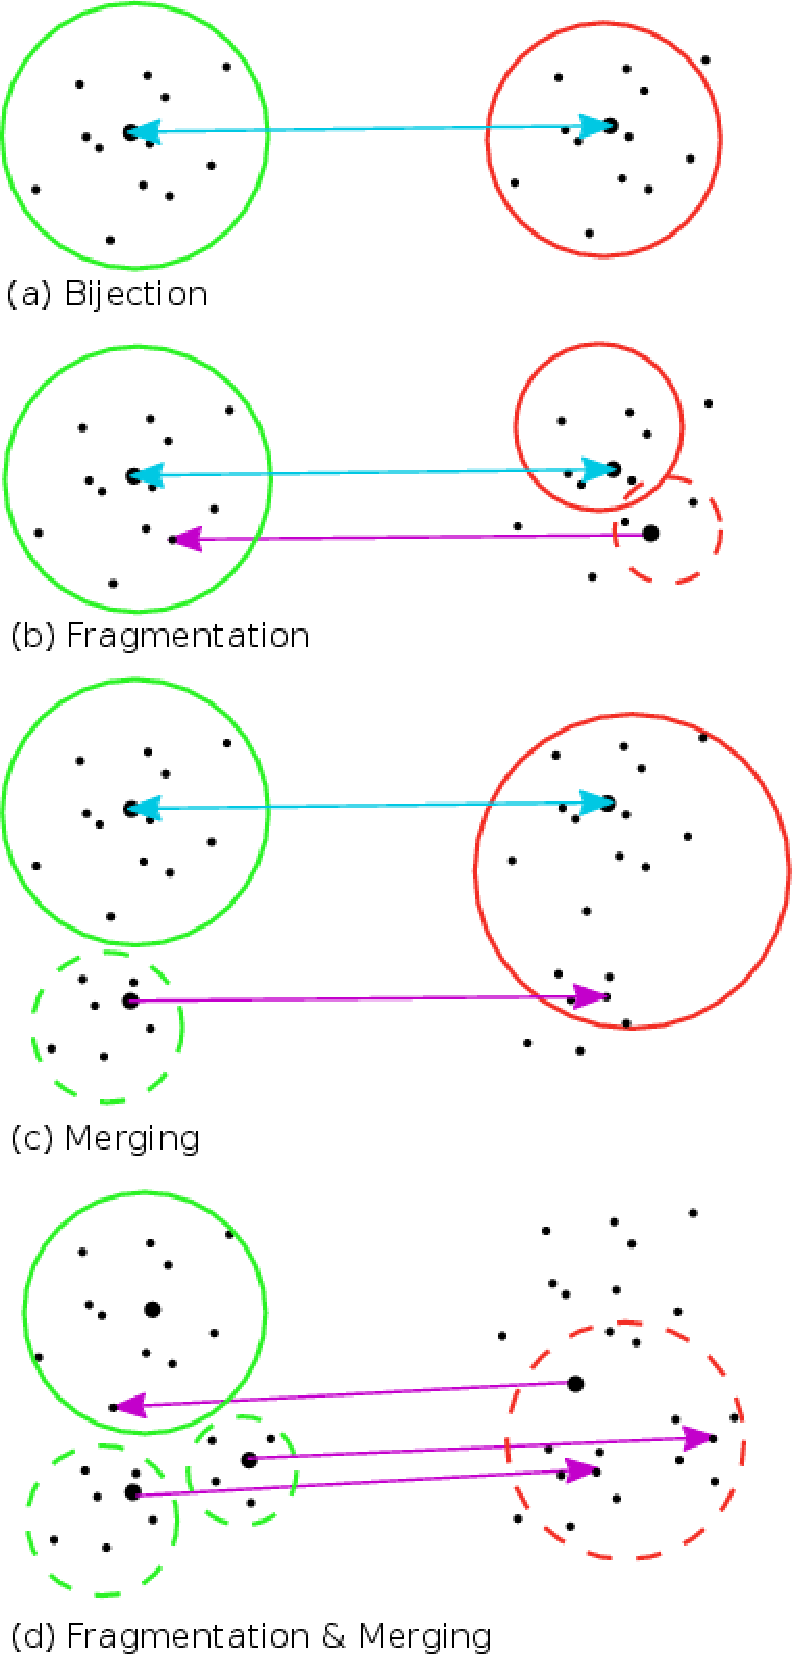
\includegraphics[width=0.3\linewidth]{figures/fof/bijection.pdf}%
    \caption{Schematic links between true groups (\emph{green circles}) and
    FoF-extracted groups, (\emph{red circles}), each with their respective
    most massive galaxy (\emph{black dots}).
    The \emph{solid circles } represent primary true and FoF groups, while the
    \emph{dashed circles} respectively correspond to secondary true groups and
    FoF fragments.
    The \emph{cyan double arrows} each indicate the one-to-one correspondence
    between the most massive galaxy in the true and extracted groups.
    The \emph{purple rightwards-pointing  arrows} correspond to the most
    massive galaxy of a true group ending up as a galaxy that is not the most
    massive of its extracted group.
    The \emph{purple leftwards-pointing arrows} represent the cases where the
    most massive galaxy of an extracted group is not the most massive of its
    parent true group.
\label{fig:CRdef}}
\end{figure}

\subsection{Global tests}

Our definition of the link between EGs and TGs allowed us to search for cases
where there is no one-to-one correspondence between the groups in real and
redshift space: a TG can suffer from  \emph{fragmentation} into several EGs,
while an EG can be built from the \emph{merging} of several TGs.

\bartreffigure{CRdef} illustrates different cases (following an analogous
figure in \citealp{Knobel+09}). The top panel shows a one-to-one correspondence
between the true and extracted groups.

We defined a fragmented TG as one that contains the MMGs of several EGs.
Multiple situations can cause fragmentation of TGs. In some cases, the FoF
algorithm fails to recover entire TGs, selecting instead its primary and
secondary substructures (see panel \bartreffigure{CRdef}b). In other cases, an
EG is mostly composed of galaxies from one TG, but the MMG of another TG is
`accidentally' linked  to the first TG\@. In consequence, the EG could be
linked to a TG providing only a single member galaxy to the EG, in comparison
with more members arising from another TG\@. When fragmentation occurred, we
distinguished the \emph{primary EG}, as that whose MMG corresponds to the MMG
of the parent TG, from the other EGs, which we called \emph{fragments}.

The dual of fragmentation is merging. In this situation, an EG contains the
MMGs of several TGs. Proceeding similarly as for the case of fragmentation, we
denoted \emph{primary TG} of a given EG the TG whose MMG corresponds to the MMG
of that EG, denoting the other TGs as \emph{secondary}. An example of merging
is shown in \bartreffigure{CRdef}c. Note that a true group can be fragmented
and its primary extracted group can be the result of a merger of the true group
with another one, as illustrated in \bartreffigure{CRdef}d.

\subsection{Local tests}
\label{sec:localtests}

Our local tests check the membership of the EGs. We defined \emph{completeness}
as the fraction of galaxies in the TG (i.e.\ within the sphere of radius
$r_{200}$) that were members of the primary EG\@. Given this definition, it did
not make sense to consider the completeness for secondary fragments, hence we
limited our tests to the primary EGs.

We defined \emph{reliability} as the fraction of galaxies in the EG that were
members of the parent TG (i.e., within the sphere of radius $r_{200}$). Here,
we also limited our tests to the primary EGs.

Mathematically speaking, these definitions of galaxy completeness, $C$, and
reliability, $R$, can respectively be written as
%
\begin{eqnarray}
    C=\rm \frac{TG \cap EG}{TG} \ ,\nonumber\\
    R=\rm \frac{TG \cap EG}{EG} \,. \nonumber
\end{eqnarray}

Looking at \bartreffigure{CRdef}, the completeness is the fraction of galaxies
in the TG (left, green circles) recovered in the EG (right, red circles), while
the reliability is the fraction of galaxies in the EG that belong to the TG\@.

These four quantities allow one to define the capacity of the FoF grouping
algorithm (or any other grouping algorithm) to recover groups in real space
from galaxy catalogs in redshift space.

Note that EGs that are fragments can have high reliability, while fragmentation
causes primary EGs to have reduced completeness. When EGs are mergers of TGs,
the secondary TGs lead to a decrease in the reliability, but can have high
completeness.

\subsection{Mass accuracy}

There are many properties of groups that one wishes to recover with optimal
accuracy (see Sect.~\ref{sec:fof_introduction}). We focused  here on one single
property that appeared to us as the most relevant: the group total mass. We
measured the masses of our EGs using the virial theorem formula of
\cite*{HTB85}
%
\begin{equation}
    M_{\rm EG} = {3\pi\over G}\,\langle R \rangle_{\rm h} \,\sigma_v^2
    = {3\pi\,N\over 2\,G}\,{\sum v_i^2\over \sum_{i<j} 1/R_{ij}}
    \ ,
\label{eq:MVT}
\end{equation}
%
where $\langle R \rangle_{\rm h} = \langle 1/R_{ij}\rangle^{-1}$ is the
harmonic mean projected separation, while $\sigma_v$ is the unbiased measure of
the standard deviation of the group velocities.

More precisely, we computed the accuracy of the log masses, respectively
defining the \emph{bias} and \emph{inefficiency} as the median and equivalent
standard deviation (half 16--84 interpercentile) of $\log (M_{\rm EG}/M_{\rm
TG})$, where $M_{\rm TG}$ is the mass of the TG within the sphere of radius
$r_{200}$ (see \bartrefsection{localtests}).

\subsection{Quality}

It is not simple to extract a unique pair of optimal LLs from the four tests
(fragmentation, merging, completeness, and reliability). To reduce the number
of tests, we combined fragmentation and merging into a single \emph{global
quality} and combined completeness and reliability into a single \emph{local
quality}.

We could define our qualities by multiplying $F$ (fragmentation) by $M$
(merging) and similarly, $C$ by $R$. However, one could alternatively multiply
$1-F$ by $1-M$, etc. Instead, we chose quality estimates that minimize the
distance to the perfect case. The advantage of using distance rather than
multiplying probabilities is that the former gives less weight to situations
where one of the two parameters is perfect and not the other. For example,
consider the case $F=M=p$. With the multiplication method, we would find that
$Q=p^2$ is also reached with $F=\epsilon\ll 1$, yielding $M_{\rm
mult}=p^2/\epsilon$, which can be quite large (hence plenty of merging). On the
other hand, with the distance method, we would find that $Q=p\sqrt{2}$ is also
reached with $F=\epsilon\ll1$ for $M_{\rm dist}\simeq p\sqrt{2}$, which is much
more restrictive. In a perfect algorithm, fragmentation and merging don't
occur, hence $F=M=0$ they are null. We therefore chose to minimize the
\emph{global quality}, defined as
%
\begin{equation}
    Q_{\rm global} = \sqrt{F^2+M^2}
\end{equation}
%
Moreover, in a perfect grouping algorithm, the EGs are fully complete and
reliable, i.e. $\langle C\rangle=\langle R\rangle=1$, where the means are over
all the groups of a mass bin. We, hereafter, drop the brackets, so that $C$ and
$R$ should now be understood as means over groups within mass bins. We then
define the \emph{local quality} as
%
\begin{equation}
    Q_{\mathrm{local}}=\sqrt{{\left(1-
    C\right)}^2+{\left(1- R\right)}^2} \,.
\end{equation}

Both global and local qualities tend to zero for a perfect galaxy group
algorithm. So the optimal LLs will be those that minimize $Q_{\rm global}$,
$Q_{\rm local}$, mass bias and mass inefficiency. The maximum possible value of
both qualities is $\sqrt{2}$.

\subsection{Scope of the tests}

We limit our tests to TGs containing at least 3 galaxies and that are not split
by the transformations of the simulation box (see \bartrefchapter{mock}).
Moreover, we only consider EGs with at least 3 galaxies and that do not lie
near the survey edges (the virial radius, 2.3 Mpc, of a true group of log mass
15.2 in solar units, placed at $z=z_{\min}=0.01$, i.e.\ at an angle of more
than $3\fdg27$) or redshift limits ($1.8\,v_{200} \approx 2.7 \,\sigma_v$, of
the same mass group, corresponding to $3073 \, \rm km \, s^{-1}$). Typically
60\% (sample 2) to 25\% (sample 6) of the groups are flagged. Finally, the
tests of galaxy completeness and reliability, as well as mass bias and
inefficiency are restricted to primary EGs of TGs (not fragments).

\section{Results}
\label{sec:results}
%
\begin{figure}
    \begin{minipage}{\linewidth}
        \centering
        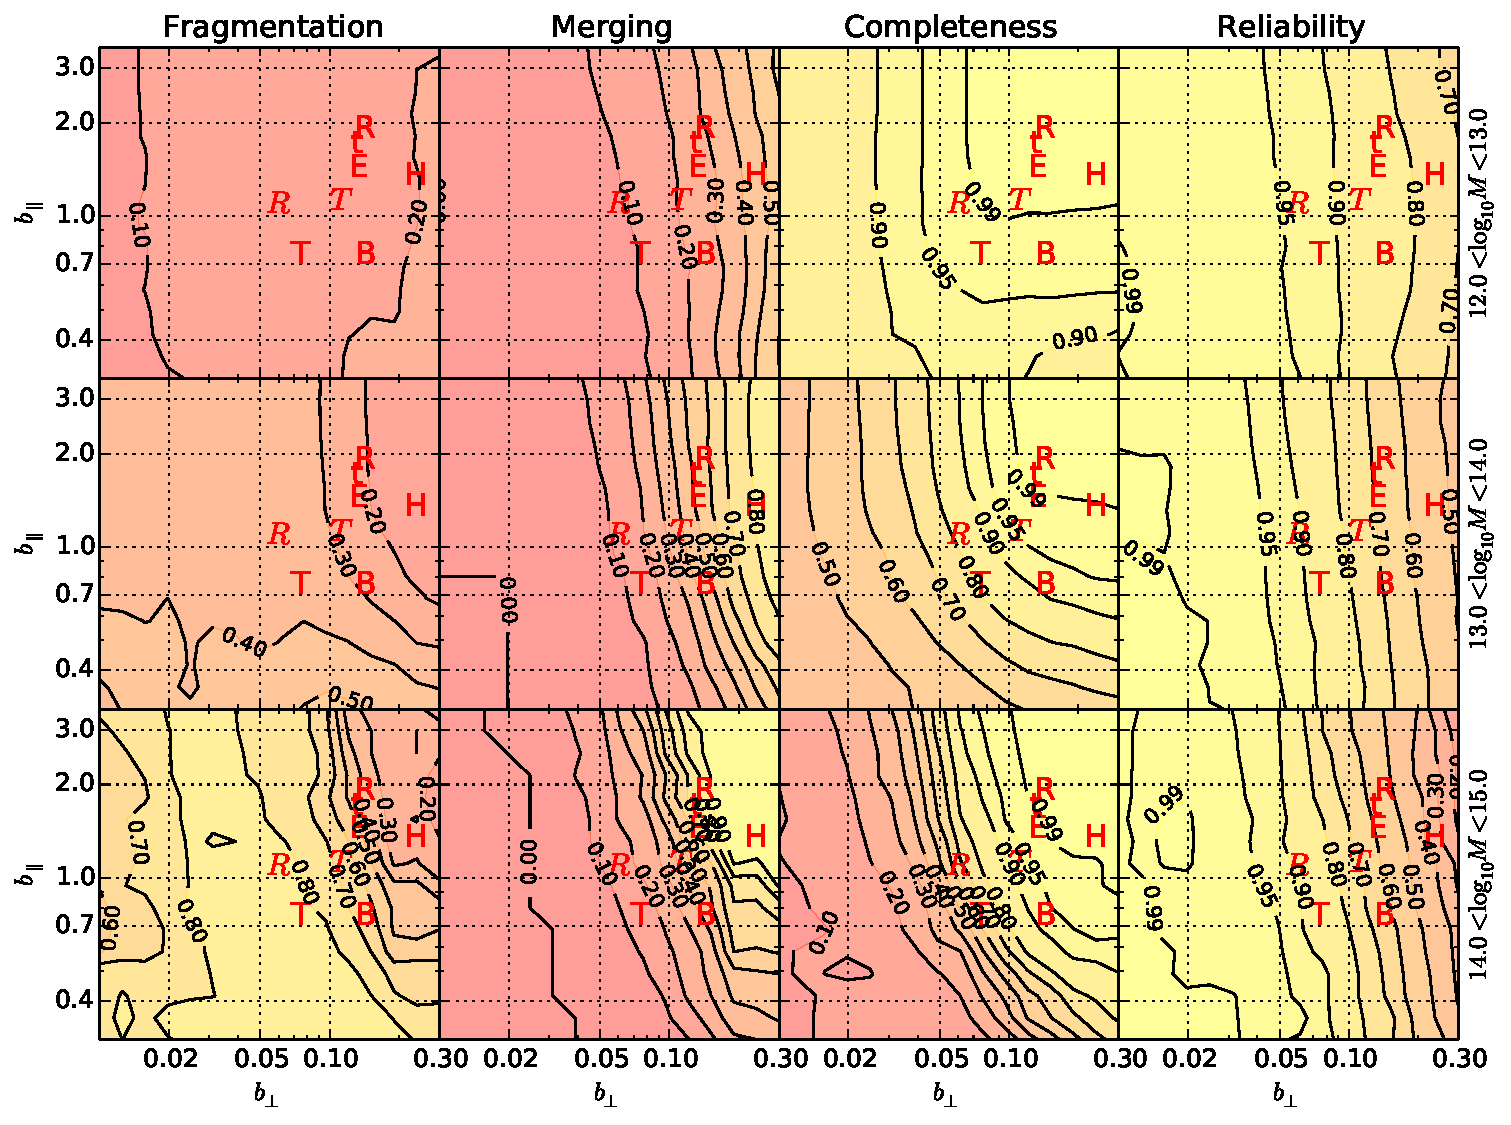
\includegraphics[height=0.415\textheight]{%
            figures/fof/results/mvir_true_1_fof_analysis.pdf%
        }
        \captionof{figure}{Contours of group fragmentation (\emph{first column}) and merging
            (\emph{second column}), as well as mean galaxy completeness
            (\emph{third column}) and reliability (\emph{fourth column}) computed
            for a 16$\times$16 grid of linking lengths for the nearby doubly
            complete galaxy subsample 2 in Table~\ref{tab:samples}. Results are
            shown for three bins of true group masses, for  unflagged groups of at
            least 3 members (for both the extracted and parent groups), and further
            restricted to primary groups in the completeness and reliability
            panels. Pairs of linking lengths corresponding to previous are also
            shown as \emph{red letters}
            (H\@: Huchra \& Geller 1982;
            R\@: Ramella et al. 1989;
            t:        Trasarti-Battistoni 1998;
            E\@: Eke et al. 2004;
            B\@: Berlind et al. 2006;
            T\@: Tago et al. 2010;
            $R$: Robotham et al. 2011;
        $T$: Tempel et al. 2014).\label{fig:test_true_small}}
    \end{minipage}
    \begin{minipage}{\linewidth}
        \centering
        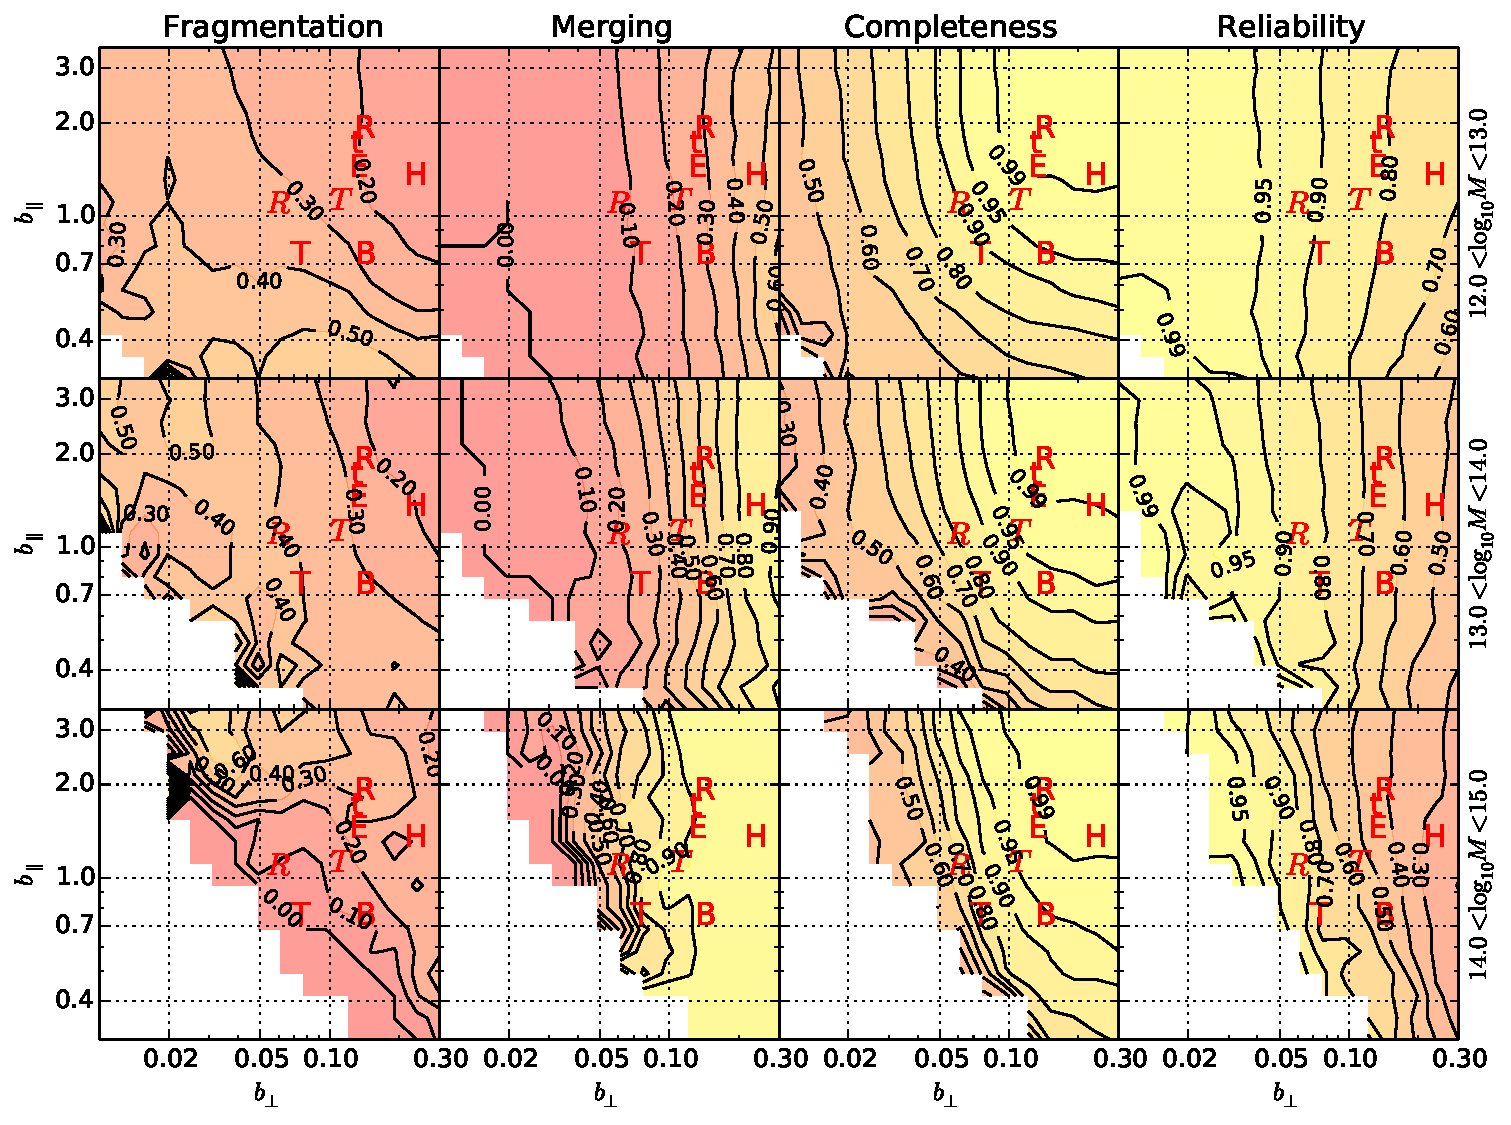
\includegraphics[height=0.415\textheight]{%
            figures/fof/results/halo_mass_1_fof_analysis.pdf%
        }
        \captionof{figure}{Same as \bartreffigure{test_true_small}, but where
        the different rows correspond to different bins of extracted group
    masses estimated from the virial theorem. The white zones show cases where
the linking lengths led to no unflagged groups extracted.
\label{fig:test_estimated_small}}
    \end{minipage}
\end{figure}
%
\begin{figure}
    \begin{minipage}{\linewidth}
        \centering
        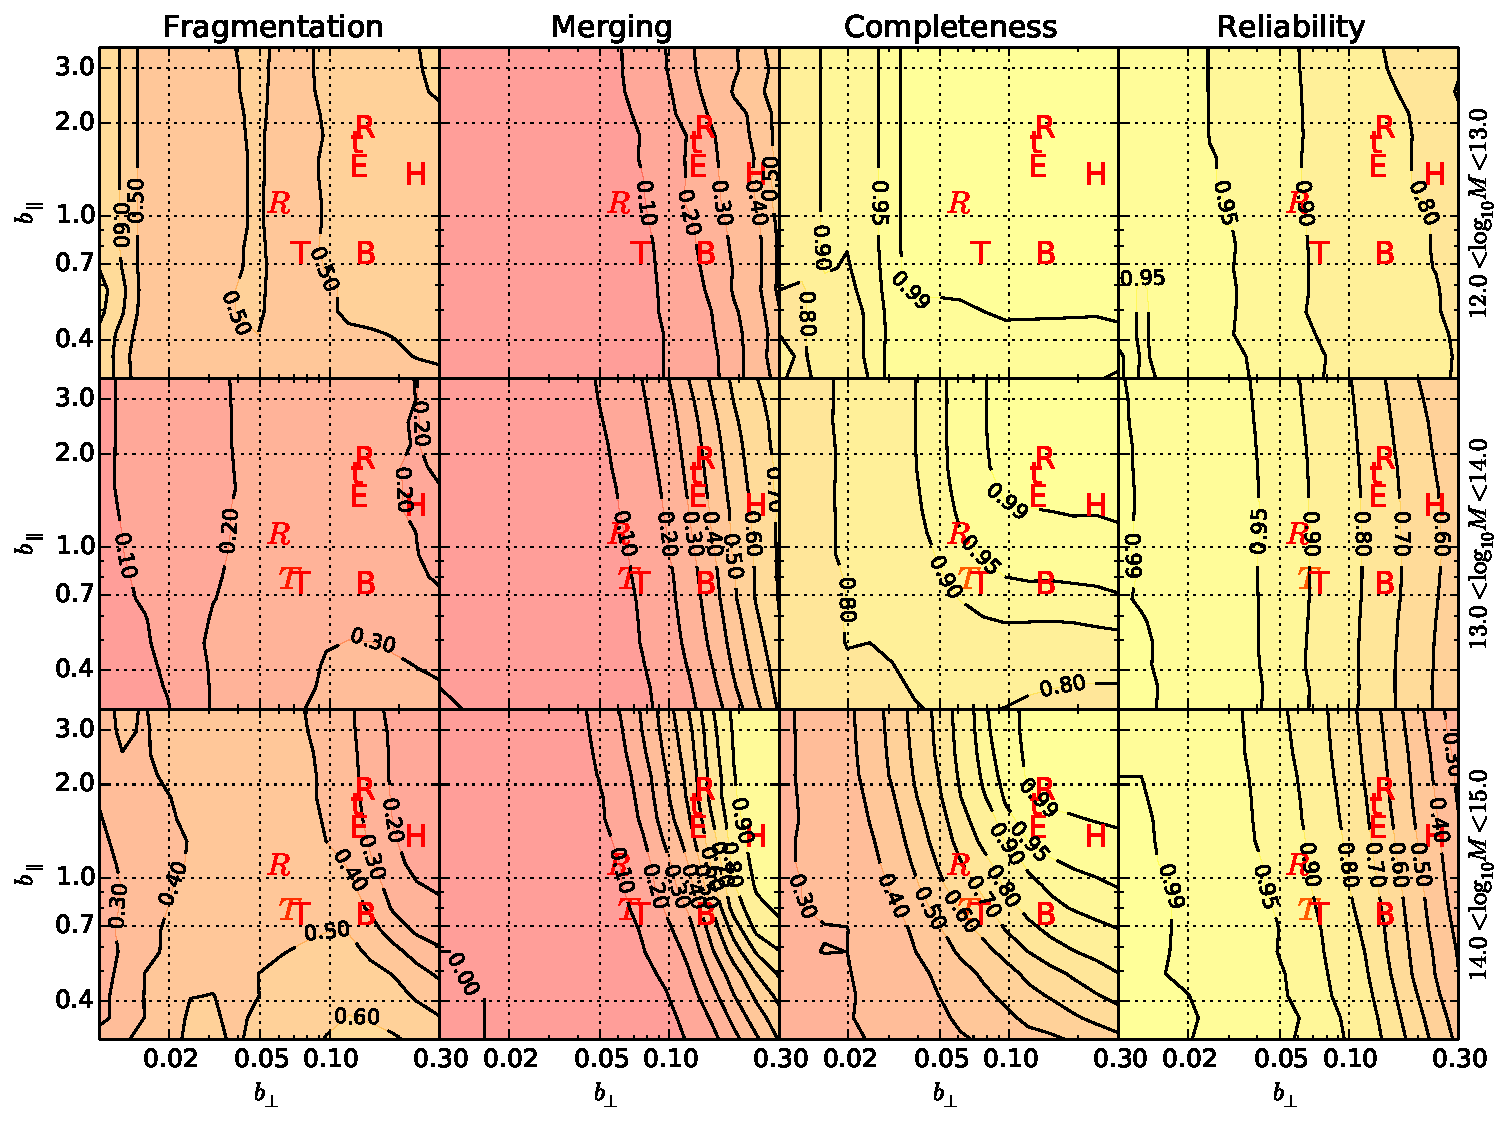
\includegraphics[height=0.415\textheight]{%
            figures/fof/results/mvir_true_5_fof_analysis.pdf%
        }
        \captionof{figure}{Same as \bartreffigure{test_true_small}, but for the
        distant doubly complete galaxy subsample 6 in
    Table~\ref{tab:samples}.\label{fig:test_true_big}}
    \end{minipage}
    \begin{minipage}{\linewidth}
        \centering
        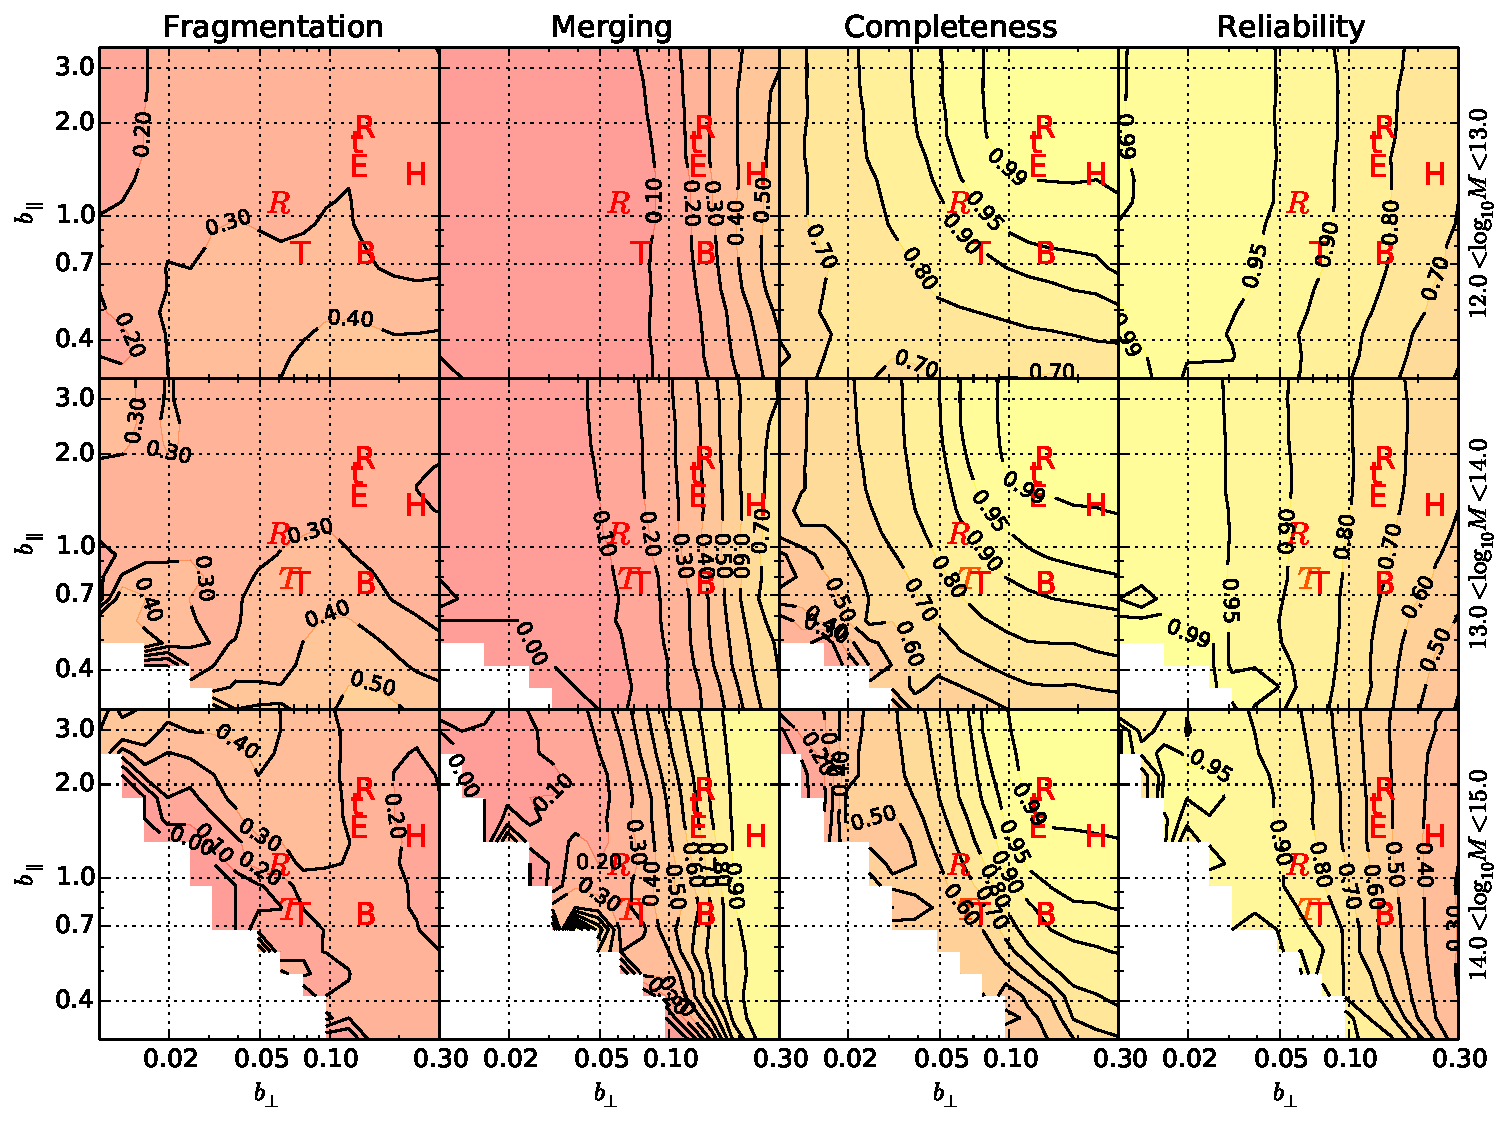
\includegraphics[height=0.415\textheight]{%
            figures/fof/results/halo_mass_5_fof_analysis.pdf%
        }
        \captionof{figure}{Same as \bartreffigure{test_true_big}, but where the
        different rows correspond to different bins of estimated
    masses.\label{fig:test_estimated_big}}
    \end{minipage}
\end{figure}
%
We have applied the FoF algorithm on near and distant doubly complete
subsamples (numbers 2 and 6 in Table~\ref{tab:samples}), repeating the tests
for a grid of 16$\times$16 geometrically-spaced pairs of LLs. The results of
our tests are shown in \bartreffigure{test_true_small} and
\bartreffigure{masses_diff}. The LLs of the different grouping studies listed
in Table~\ref{tab:groupalgos} are shown, except for~\cite{MZ02}, whose LLs
nearly overlap with those of~\cite{Eke+04}.

\subsection{Group fragmentation and merging}

\bartreffigure{test_true_small} indicates that, for the nearby doubly complete
subsample (number 2), fragmentation only affects the massive TGs (up to
$\approx$80\% of them for popular LLs), while
\bartreffigure{test_estimated_small} shows that, for popular LLs, the
fragmentation is lower (10--30\%) at high EG mass, hence fragment masses tend
to be small (typically 20--40\% fragmentation at small and intermediate
estimated masses).

On the other hand, the distant doubly complete subsample behaves in almost the
opposite manner: fragmentation is most important at the lowest TG masses
(roughly 50\% fragmentation, \bartreffigure{test_true_big}) and is independent
of estimated EG masses (at roughly 20--30\%,
\bartreffigure{test_estimated_big}).

In any event, fragmentation tends to decrease with greater linking lengths, as
expected, although it decreases somewhat faster with increasing $b_\perp$ than
with increasing $b_\parallel$.

Since merging is the dual of the fragmentation, one expects the level of
merging to vary  in the opposite way as fragmentation. Indeed,
\bartreffigure{test_estimated_small} and \bartreffigure{test_estimated_big}
indicate that merging becomes more important at higher estimated masses,
respectively reaching up to 90\% and 65\% for high estimated masses with
popular choices of LLs in subsamples numbers 2 and 6. However,
\bartreffigure{test_true_small} and \bartreffigure{test_true_big} shows that
the merging fraction increases only slowly with TG increasing mass, with
typically 15--40\% (increasing fast with $b_\perp$) of the TGs being merged with
other ones. Finally, merging decreases with smaller LLs, especially with
smaller $b_\perp$.
%
\begin{figure*}
    \centering
    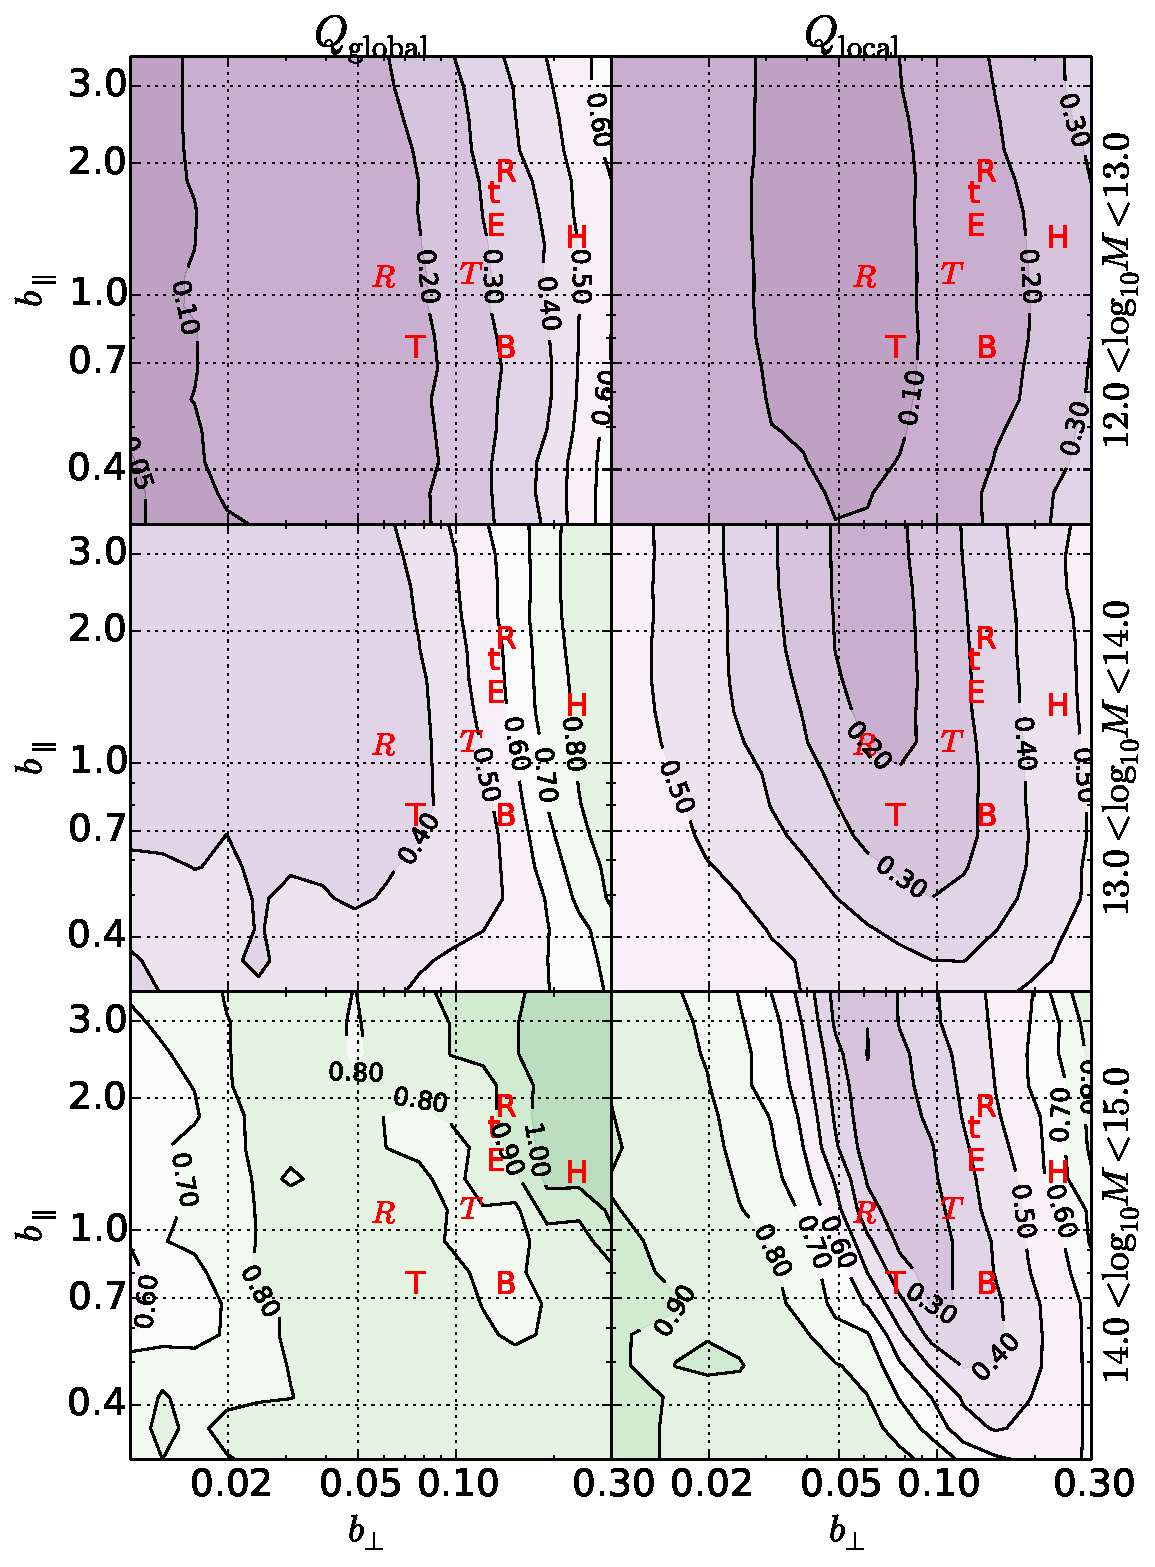
\includegraphics[height=0.4\textheight]{%
        figures/fof/results/mvir_true_1_quality_fof_analysis.pdf%
    }
    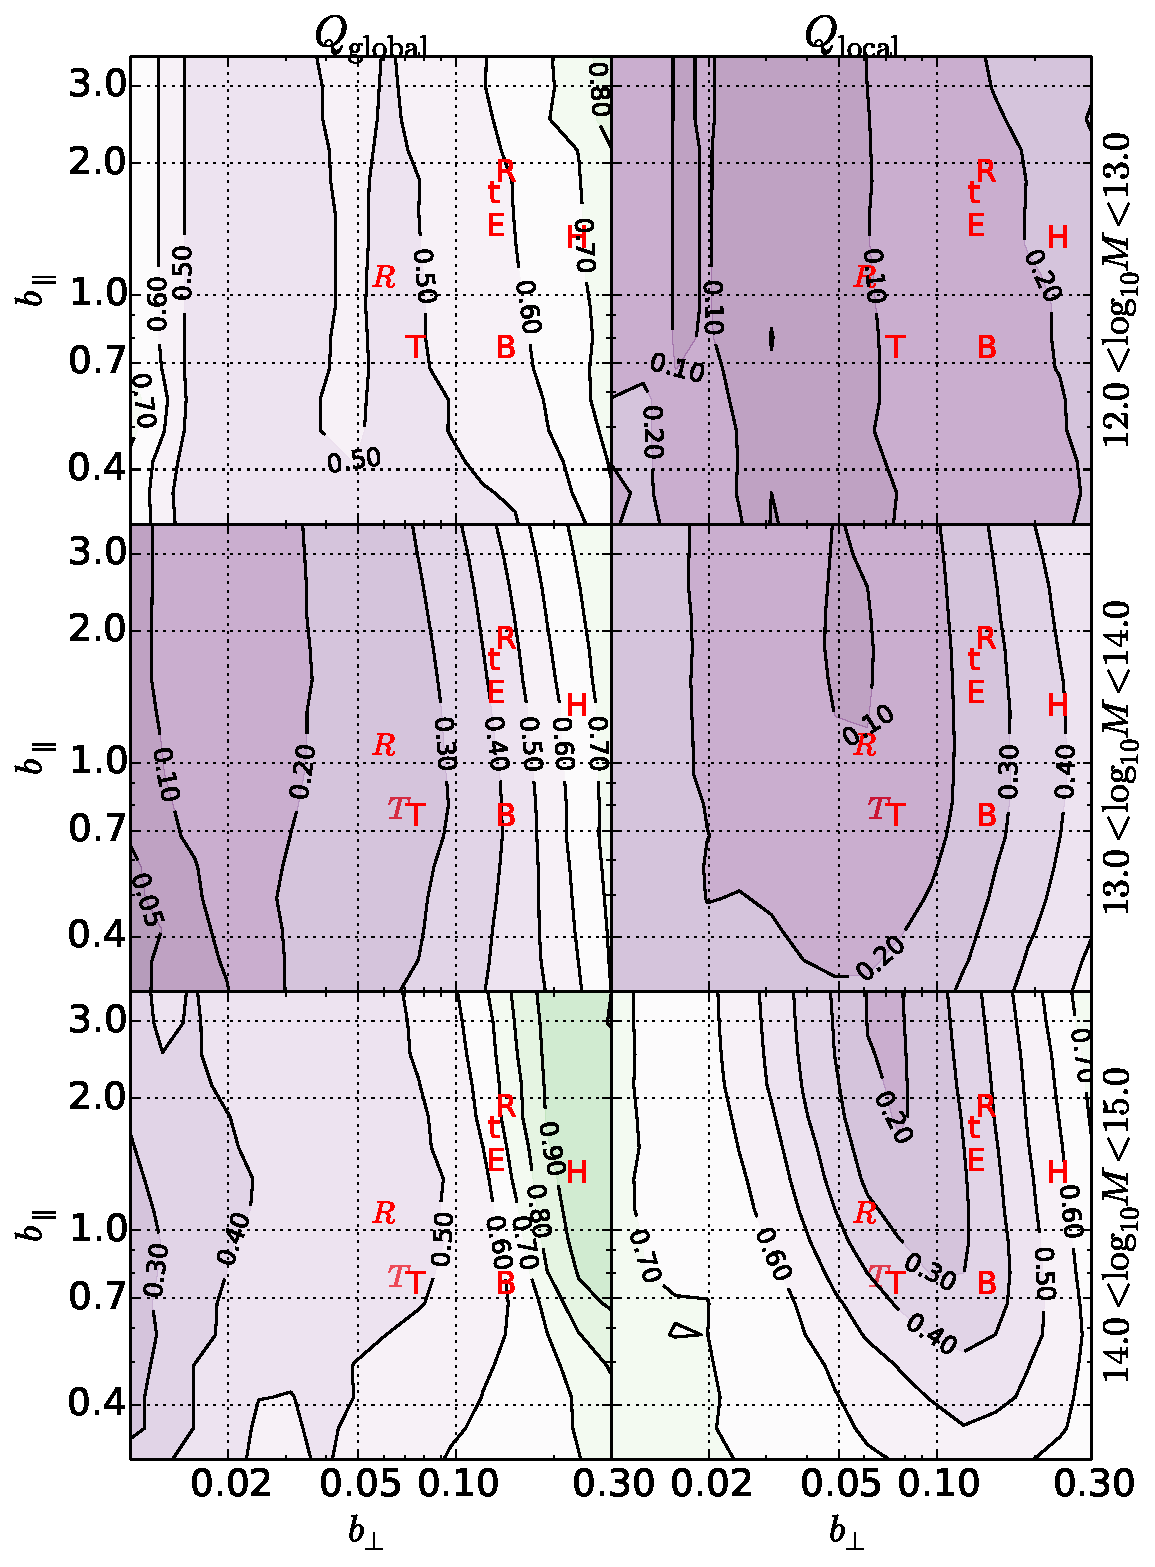
\includegraphics[height=0.4\textheight]{%
        figures/fof/results/mvir_true_5_quality_fof_analysis.pdf%
    }
    \caption{Global and local quality factors in a 16$\times$16 grid of linking
        lengths for subsamples 2 (\emph{left}) and 6 (\emph{right}), in three
        bins of true masses Results are shown for unflagged groups (restricted
        to primary groups for $Q_{\rm local}$) of at least 3 members (in both
    the true and extracted group). The symbols are as in
\bartreffigure{test_true_small}\label{fig:quality_true}}.
\end{figure*}
%
\begin{figure*}
    \centering
    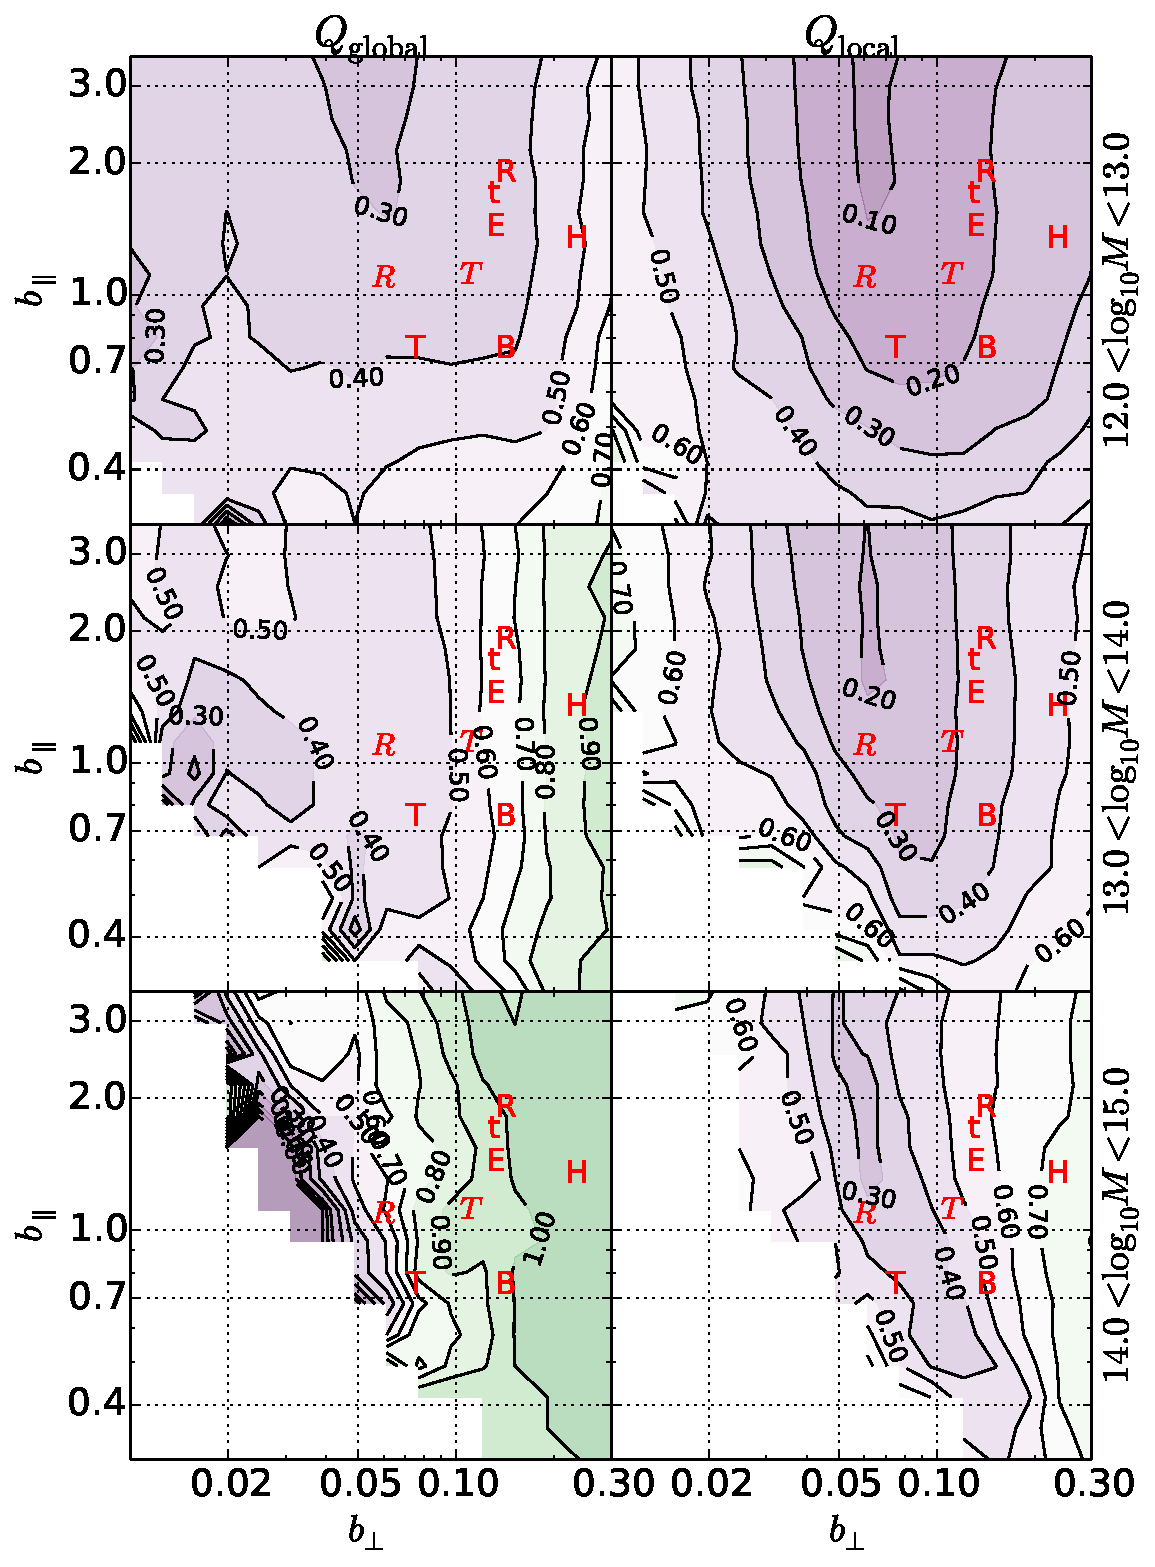
\includegraphics[height=0.4\textheight]{%
        figures/fof/results/halo_mass_1_quality_fof_analysis.pdf%
    }
    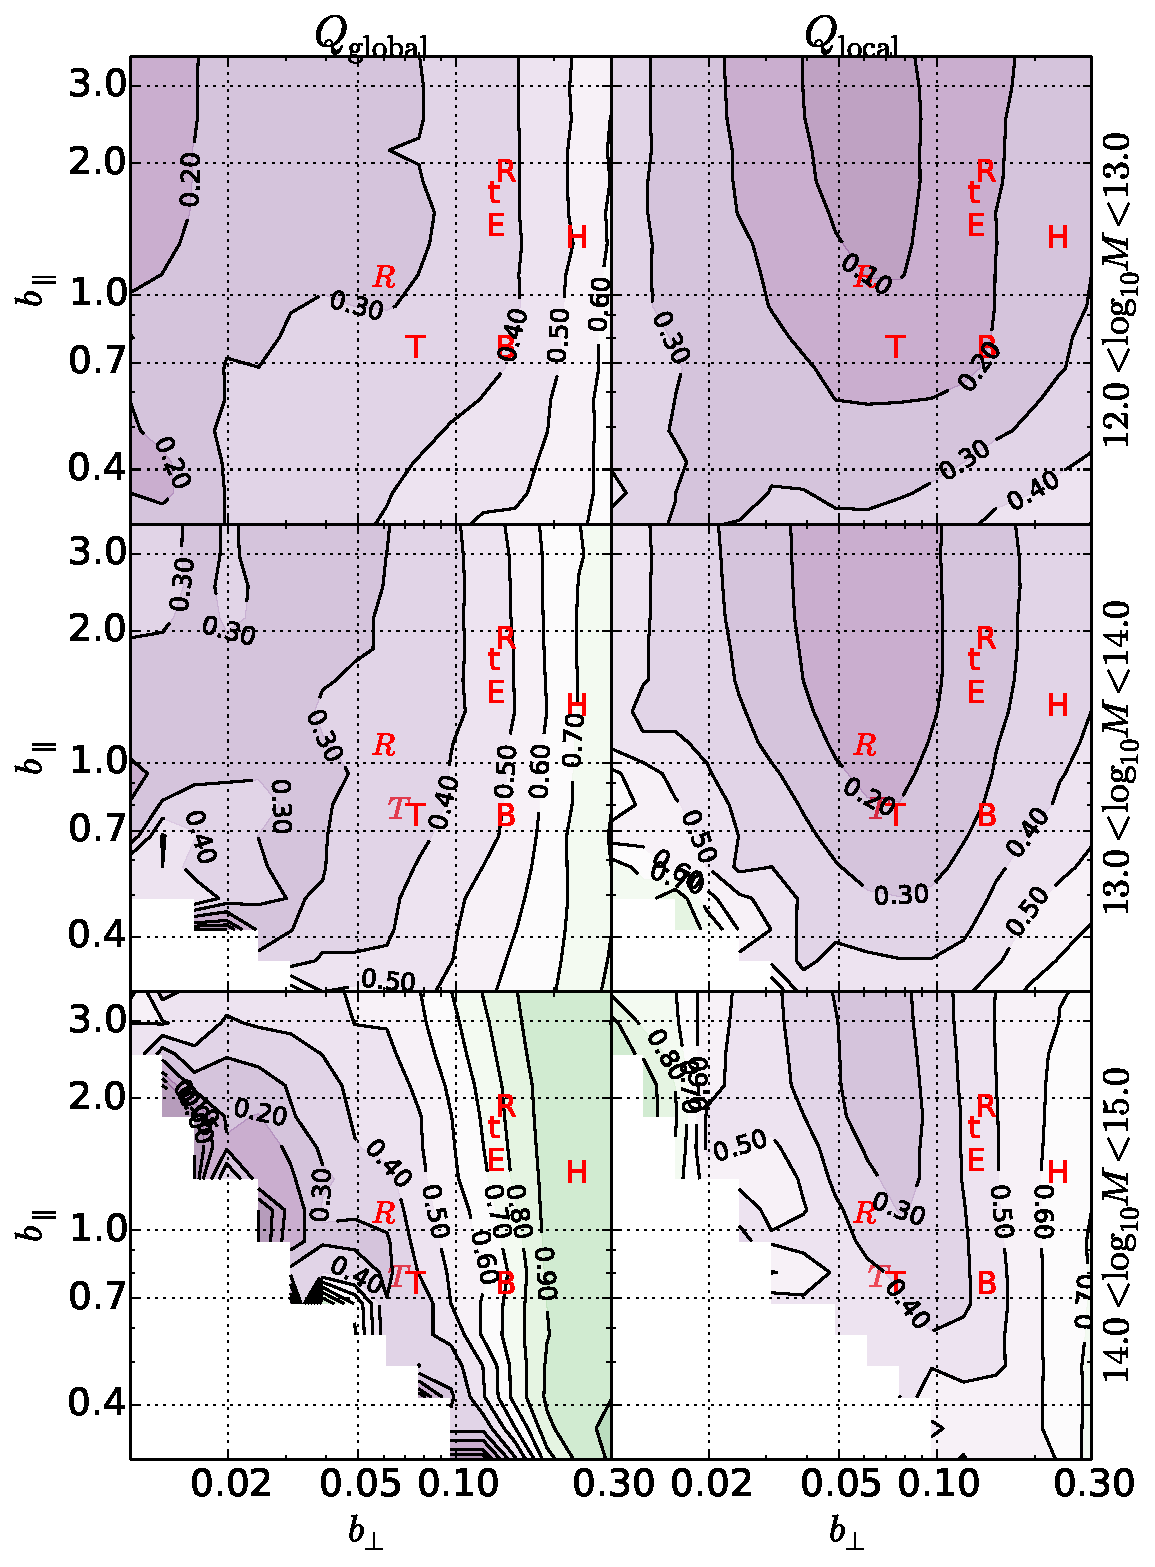
\includegraphics[height=0.4\textheight]{%
        figures/fof/results/halo_mass_5_quality_fof_analysis.pdf%
    }
    \caption{Same as \bartreffigure{quality_true} but in bins of estimated
    masses. The white zones show cases where the linking lengths led to no
unflagged groups extracted.\label{fig:quality_estimated}}
\end{figure*}

\bartreffigure{quality_true} and \bartreffigure{quality_estimated} show the
$Q_{\rm global}$ quality indicator that combines fragmentation and merging into
a single parameter. These figures show that decreasing $b_\perp$ leads to a
better tradeoff between fragmentation and merging, i.e.\ that the decrease of
merging with decreasing $b_\perp$ has a stronger effect than the increase of
fragmentation with decreasing $b_\perp$: the optimal $Q_{\rm global}$ is often
reached for $b_\perp < 0.02$.

\subsection{Galaxy completeness and reliability}

\bartreffigure{test_true_small} and \bartreffigure{test_true_big} indicate that
completeness is very high ($>99\%$) at low TG masses, and decreases to lower
values ($60-99\%$) at high TG mass. A weaker trend occurs when EG mass is
substituted for TG mass (see \bartreffigure{test_estimated_small} and
\bartreffigure{test_estimated_big}). Since high mass TGs are less complete,
their estimated masses should be smaller, and the EGs with high masses will be
the lucky complete ones, which explains the weaker trend of completeness with
EG mass. Note that we are only considering primary groups of at least 3
members. The transverse and LOS linking lengths have roughly the same impact on
galaxy completeness.

The reliability of the group membership decreases with increasing EG mass
(\bartreffigure{test_estimated_small} and \bartreffigure{test_estimated_big}):
regardless of the subsample, the reliability is 80--90\% for low mass EGs, but
only 50--85\% for high mass EGs. The value of $b_\parallel$ has virtually no
effect on galaxy reliability. We will discuss this lack of convergence of the
reliability with $b_\parallel$ in \bartrefsection{discussion}.

Galaxy reliability also decreases with the masses of the TGs, but the trend is
weaker (\bartreffigure{test_true_small} and \bartreffigure{test_true_big}): as
the reliability decreases from 85--95\% to 60--90\%, roughly independent of the
subsample.

The right panels of \bartreffigure{quality_true} and
\bartreffigure{quality_estimated} show that, again, the transverse LL appears
to be more decisive than the LOS one when combining galaxy completeness and
reliability into a single local quality factor.

\subsection{Mass accuracy}
%
\begin{figure}[t]
    \centering
    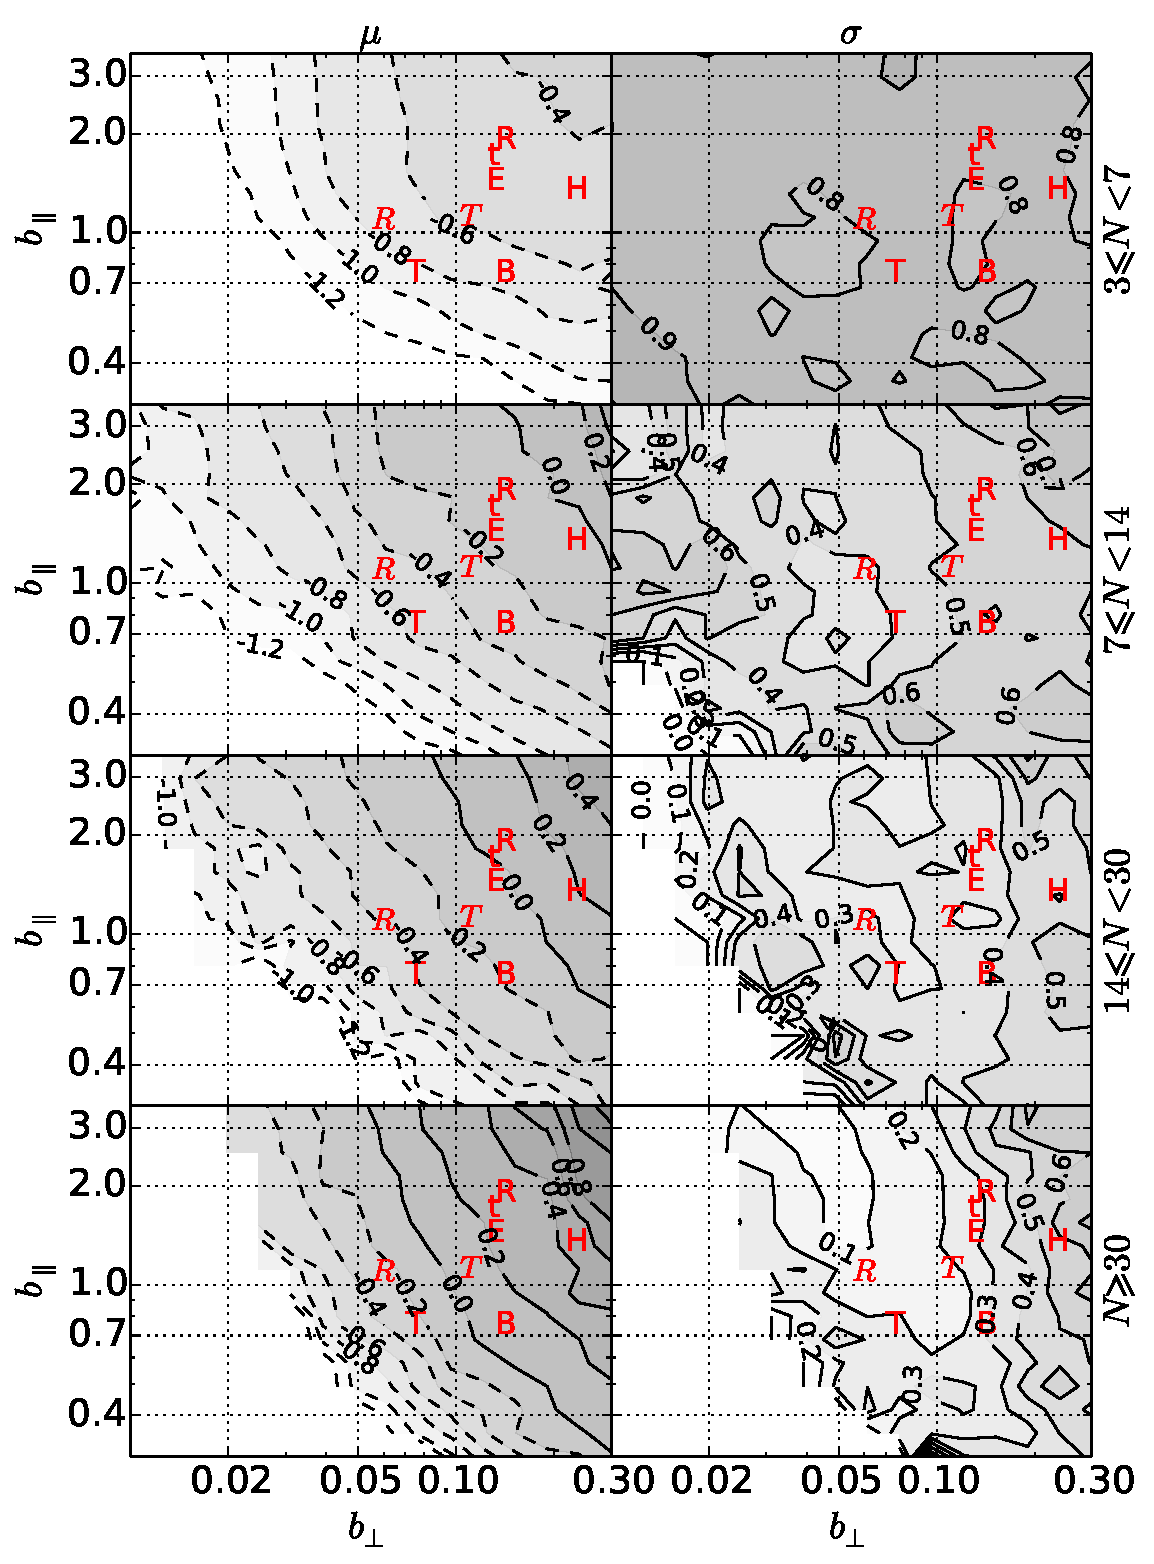
\includegraphics[height=0.44\textheight]{%
        figures/fof/results/1_fof_analysis_masses.pdf%
    }
    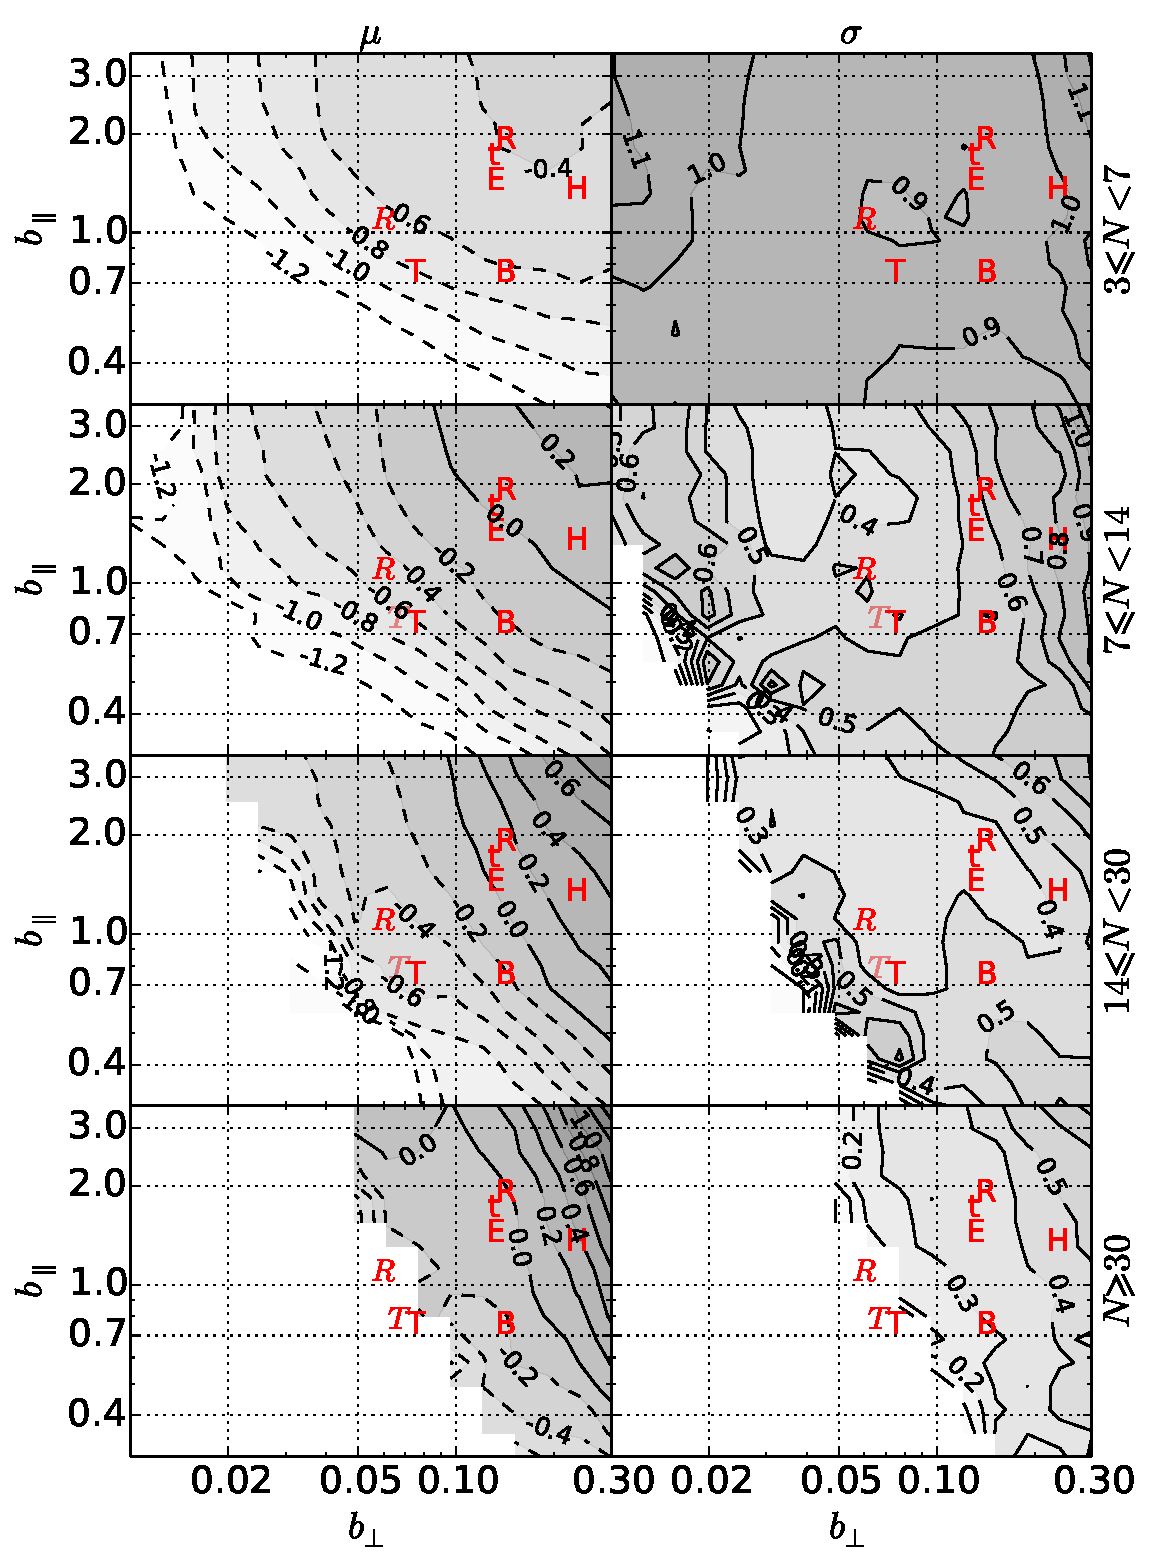
\includegraphics[height=0.44\textheight]{%
        figures/fof/results/5_fof_analysis_masses.pdf%
    }
    \caption{Bias ($\mu$) and inefficiency ($\sigma$) of the group masses
        estimated  by the virial theorem (\bartrefequation{MVT}) on our
        16$\times$16  grid of linking lengths, in four bins of extracted group
        richness (we do not consider extracted groups for which the parent true
        group has $\leq3$ members). The bias and inefficiency are respectively
        computed as the median and half 16--84 interpercentile of
        $\log_{10}\left(M_{\rm EG}/M_{\rm TG}\right)$. Results are shown for
        primary, unflagged groups. The left and right panels are respectively
        for galaxy subsamples 2 and 6. The symbols are as in
        \bartreffigure{test_true_small}. The white zones indicate linking
        lengths with no unflagged groups extracted.\label{fig:masses_diff}}
\end{figure}

The left columns  of the two panels of \bartreffigure{masses_diff} show that
the primary EG masses recovered by the FoF algorithm are systematically biased
low: for the popular choices of LLs, the bias ($\mu$) is as strong as
$-0.6\pm0.2$ dex at low multiplicity ($N_{\rm EG}\leq 6$), decreasing to
$0.0\pm0.3$ dex at high multiplicity ($N_{\rm EG}\geq 30$).

The right columns of the two panels of \bartreffigure{masses_diff} indicate
that, even if the biases could be corrected for, the masses cannot be recovered
to better than 0.8--0.9 dex at low multiplicity, improving to 0.2 dex at high
multiplicity. The  inefficiency ($\sigma$) is minimal for $b_\perp \approx
0.05$ (within a factor 2) and $b_\parallel \approx 1.0$ (low richness) or
$b_\parallel \ga 1.0$ (intermediate and high richness). For transverse LLs
within 40\% of $b_\perp=0.1$, the inefficiency is not very insensitive to
$b_\parallel$.

The situation becomes even worse when fragments are included in the statistics.
In this work, we have separated the accuracy of the group masses with the
occurrence of group fragmentation. But observers cannot tell if a group is a
fragment or a primary EG\@.

\section{Conclusions and Discussion}
\label{sec:discussion}

Before testing the FoF algorithm using a mock galaxy catalog in redshift space,
we first argued on physical grounds (\bartrefsection{fofpred}) that the
normalized transverse linking length, ought to be $b_\perp \approx 0.10$
(slightly increasing with richness) to extract 95\% of the galaxies within the
virial radius of NFW true groups.  We also argued that, restricting the
galaxies along the line-of-sight to $\pm1.65\,\sigma_v$ (95\% of the galaxies)
for groups defined to be 200 times denser than the critical density of the
Universe, requires $b_\parallel/b_\perp \approx 11$, hence $b_\parallel \simeq
1.1$. These LLs are estimated from our mocks that are based upon the
Millennium-II simulation that had adopted $\Omega_{\rm m}=0.25$. Converting to
$\Omega_{\rm m}=0.3$ yields $b_\perp=0.11$ and $b_\parallel=1.3$. Finally,
estimating the contamination by interlopers, we predict between 80\% (NFW model
extended outwards) to 90\% (NFW model truncated to sphere plus random
interlopers) galaxy reliability.
%
\begin{figure}[t]
    \begin{minipage}{0.5\linewidth}
        \centering
        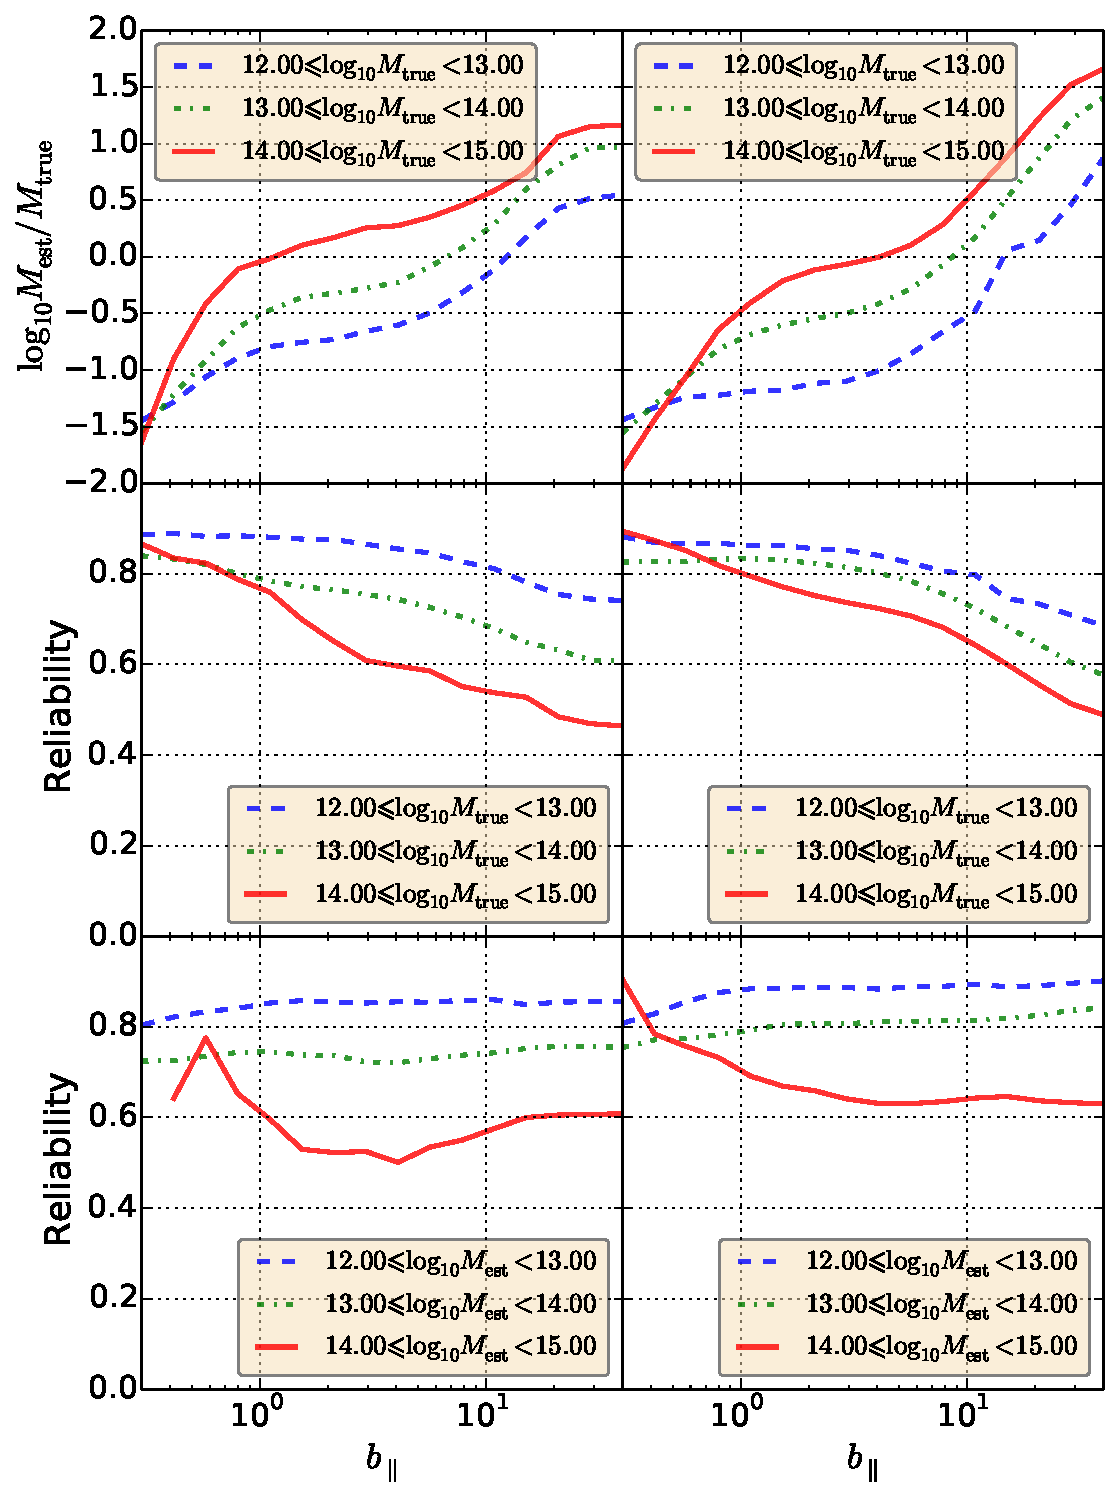
\includegraphics[width=0.85\linewidth]{%
            figures/fof/parallel_link_behaviour.pdf%
        }
        \captionof{figure}{Variation of the mass bias and reliability as a
        function of $b_\parallel$ for $b_\bot =0.1$, for subsamples 2
    (\emph{left}) and 6 (\emph{right}).\label{fig:parallel_behaviour}}
    \end{minipage}
    \begin{minipage}{0.5\linewidth}
        \centering
        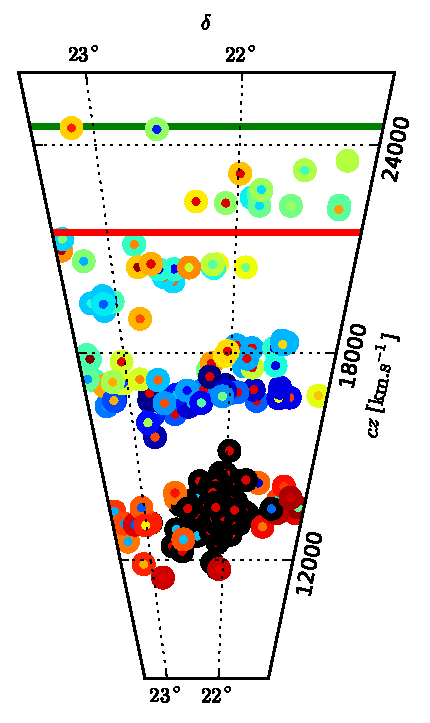
\includegraphics[width=0.6\linewidth]{figures/fof/group_halo.pdf}
        \captionof{figure}{An example of group and halo for $b_\parallel=20.8$
            and $b_\bot=0.1$ for subsample 4. The width of the cone is
            exaggerated by a factor of roughly 5 for illustrative purposes.
            \emph{Outer} and \emph{inner circle colors} respectively refer to
            the TGs and EGs. The \emph{horizontal green} and \emph{red lines}
            respectively indicate the maximum redshift, $z_{\max}$ and the
            redshift where galaxies are flagged for being close to $z_{\max}$.
            Some galaxies of the red EG, whose TG is the black one, are flagged
            for being close to $z_{\max}$, hence the group would not be
        considered in our tests.\label{fig:group}}
    \end{minipage}
\end{figure}

We then built a mock redshift space galaxy catalog with the properties of the
flux-limited SDSS primary spectroscopic sample, from which we extracted 2
subsamples that are doubly complete in distance and luminosity
(\bartrefchapter{mock}). We then extracted groups from both of these
subsamples, running the standard FoF algorithm for $16\times16$ pairs of
linking lengths.  In each case, we measured the fraction of true groups that
were fragmented in the FoF extraction process, the fraction of extracted groups
that were built by the merging of several true groups, as well as the bias and
inefficiency with which the group masses were extracted. Moreover, we computed
the completeness and reliability of the galaxy membership relative to the
spheres of radius $r_{200}$ in which the true groups are defined.

We analyzed group fragmentation, merging, galaxy completeness and reliability,
mass bias and inefficiency for two doubly complete subsamples and in bins of
true and estimated mass or estimated richness (for the mass accuracy).

We found that massive true groups are more prone to fragmentation, as expected,
but that, for popular choices of linking lengths, the probability of
fragmentation is greatest (30\%) at low estimated mass, i.e.\ the fragments are
of low mass. The process of fragmentation of rich (massive) groups  is similar
to images of large galaxies being preferentially fragmented by automatic image
extraction pipelines (e.g., \citealp{DePropris+07}).

Group merging is low at low estimated mass, but increases drastically to reach
40--90\% (for popular linking lengths) at high estimated mass. Galaxy
completeness is high, typically $>80\%$. Galaxy reliability is typically 75 to
90\% depending on group mass..

Our analytical prediction of 95\% completeness for $b_\perp\simeq 0.10$ is only
met for groups of high true masses (\bartreffigure{test_true_small} and
\bartreffigure{test_true_big}). Groups of low mass will have more concentrated
galaxy populations, which will lead to smaller values of ${\rm
Max}(S_\perp)/r_{200}$, hence smaller values of $b_\perp$. Also, our analytical
prediction of 80--90\% reliability for groups with $b_\perp=0.10,
b_\parallel=1.1$ is accurate for groups of all masses of the distant subsample
(\bartreffigure{test_true_big}). However, for the nearby subsample (2), our
predicted reliabilities are only \nobreak{accurate} for groups of low true
masses, but optimistic for higher mass groups, for which $R \simeq 70-75\%$.

Group merging and galaxy reliability depend little on $b_\parallel$, especially
at high transverse linking length, $b_\perp > 0.1$, where the galaxies are
extracted to projected radii beyond $r_{200}$, hence the contamination by
interlopers is mainly in the transverse direction. The lack of optimal
$b_\parallel$ for galaxy reliability may seem surprising at first. We checked
our analysis by measuring the reliability for $b_\perp=0.1$, for a very wide
range of $b_\parallel$ extending from 0.3 to 40.
%
The top panels of \bartreffigure{parallel_behaviour} indicate that the
reliability does end up decreasing fairly fast beyond some large value of
$b_\parallel \simeq 6$, i.e.\ beyond the limits of
\bartreffigure{test_true_small} and \bartreffigure{test_true_big}. The second
row of panels of \bartreffigure{parallel_behaviour} show a different behavior
in bins of estimated mass. This is the consequence of the estimated mass
increasing very fast with $b_\parallel$, as shown in the bottom panels of
\bartreffigure{parallel_behaviour}. The increase, with increasing
$b_\parallel$, of the mass bias is roughly parallel to the corresponding
decrease of the reliability (in bins of TG mass). At low $b_\parallel$, the
reliability decreases fairly rapidly and the mass bias increases rapidly
(towards zero), then both settle into an almost constant plateau in the range
$1.4 \la b_\parallel \la 8$, then both worsen rapidly up to $b_\parallel\simeq
25$, beyond which both saturate, because the longitudinal link is so large that
one reaches the minimum and maximum redshifts of the subsample, where most
groups are flagged. Massive groups that are built from TG merging can be fairly
reliable if the secondary TGs have negligible mass relative to the primary one.
This explains why $R$ remains fairly high when $M$ is high. The plateau around
\bpar$\approx 3$ appears to represent the range of optimal longitudinal LLs.

An illustration is given in \bartreffigure{group}, where a given EG has
reached the limits of the catalog with a very large value of \bpar{}.
\bartreffigure{group} also shows that interloping TGs are highly clustered.
This may explain why increasing $b_\parallel$ has only a small effect on
galaxy reliability: there is a void behind the main TG (black outer
circles).

While fragmentation, measured in bins of true group mass, decreases with
increasing $b_\parallel$, as expected (\bartreffigure{test_true_small} and
\bartreffigure{test_true_big}), we find that in bins of estimated mass, the
fraction of groups that are (secondary) fragments increases with $b_\parallel$
(\bartreffigure{test_estimated_small} and \bartreffigure{test_estimated_big}).
We believe that this is caused by interlopers increasing the group estimated
mass (\bartreffigure{parallel_behaviour}).

The masses, estimated with the virial theorem (\bartrefequation{MVT}) are a
strong function of the multiplicity of the extracted group. The estimated
masses are systematically biased low, especially for low extracted group
multiplicities (typically by a factor 4!). Similar trends have been found for
FoF groups \citep{Robotham+11} and for other, mostly dynamical, group mass
estimators \citep{Old+14}. The estimated group masses are inaccurate, even
after correcting for the biases: the typically errors are 0.8--0.9 dex at low
multiplicity, decreasing to 0.3 dex at high multiplicity.

The optimal completeness and reliability of the galaxy membership lead to
fairly extreme linking lengths, i.e. $b_\perp < 0.1$ and $b_\parallel > 2$.
However, the use of such a small transverse linking length amounts to
extracting the inner regions of groups, thus missing their outer envelopes.
Indeed, one notices that fragmentation worsens at increasingly lower values of
$b_\perp$. Therefore, our attempt to define a local quality by combining galaxy
completeness and reliability is of little use if one wishes to recover galaxies
out to close to the virial radii of groups.

In fact, the optimal linking lengths depend on the scientific goal:
%
\begin{itemize}
    \item statistical studies of environmental effects require high reliability
        (say $R>  0.9$), accurate masses and, to a lesser extent, minimal
        fragmentation.
    \item cosmographical studies of group mass functions require accurate
        masses, minimal group merging and fragmentation.
    \item studies for followups at non-optical wavelengths (e.g. X-rays),
        benefit from high completeness.
\end{itemize}

For statistical studies of environmental effects, it seems best to adopt
$b_\perp \simeq 0.06$, $b_\parallel \approx 1.0$, for which the reliability is
roughly as high as it gets for the choice of $b_\perp$: over 90\% at low
$M_{\rm EG}$ and over 80\% at intermediate and high $M_{\rm EG}$. Then,  the
completeness is higher than 70\% at high estimated mass and much higher at low
$M_{\rm EG}$. The mass inefficiency is minimal, but with this choice of LLs,
there will be virtually no EGs with more than 30 galaxies in the distant more
luminous subsample (\bartreffigure{masses_diff}).

This choice of LLs is close to that of~\cite{Robotham+11}, which may seem
obvious since both studies used some form of optimization of the LLs. However,
the details of the optimization criteria are somewhat different:
\citeauthor{Robotham+11} multiplied four criteria: basically the group
completeness and reliability, which bears some resemblance to our group
fragmentation and merging, but theirs is based on TG-EG pairs that have more
than half their galaxies in common, as well as two measures of a combination of
galaxy completeness and reliability, averaged over TGs and EGs respectively.
Our analysis differs in that we directly constrained group fragmentation and
merging, as well as galaxy completeness and reliability for primary fragments,
and finally mass accuracy.

For cosmographical and other studies involving accurate group mass functions,
it appears best to adopt $b_\perp \simeq 0.05$, $b_\parallel \simeq 2$, as
lower $b_\parallel$ increases fragmentation
(\bartreffigure{test_estimated_small} and \bartreffigure{test_estimated_big}),
while higher $b_\parallel$ causes too high group fragmentation at high EG
masses. This value of $b_\parallel\simeq 2$ is in agreement with the
intersection of the regions of $(b_\perp,b_\parallel)$ space  that optimize
both the multiplicity function  and velocity dispersions obtained by
\cite{Berlind+06}.

Finally, for non-optical followups, for which galaxy completeness is perhaps
the sole important parameter, one should privilege large linking lengths, e.g.
$b_\perp \simeq 0.2$, $b_\parallel \simeq 2-4$. However, one can also adopt
$b_\perp = 0.1$, $b_\parallel \simeq 2-4$, for which the completeness is
greater than 95\% at all masses and for both subsamples.

Converting from $\Omega_{\rm m} = 0.25$ (Millennium-II Simulation) to
$\Omega_{\rm m} = 0.3$ (WMAP-Planck compromise), $b_\perp$ must be increased by
6\% (\bartrefequation{bperpfromDelta}) to $b_\perp \simeq 0.07$ for the choices
optimizing environmental or cosmographical studies. Since $b_\parallel/b_\perp$
is independent of $\Omega_{\rm m}$ at given $\Delta$, \bpar{} must also be
increased by 6\%, i.e.\ to \bpar$\approx1.1$ for environmental studies.

We finally note that while high estimated mass group fragmentation  and merging
depends on the particular doubly complete subsample, galaxy completeness and
reliability as well as mass accuracy depend little on the
subsample.~\cite{Berlind+06} had similarly concluded that the doubly complete
subsample influenced little their tests of the group multiplicity function and
the accuracy of projected radii and velocity dispersions.

FoF grouping techniques can be used as a first guess for other more refined
grouping methods \citep{YMvdBJ05,Yang+07}. In a future paper \citep{DM14b}, we
will present another grouping algorithm, which is not an FoF, but is instead a
probabilistic grouping algorithm that is built upon our current knowledge of
groups and clusters (partly from X-rays and independent of FoF analyses of
optical galaxy samples) and from cosmological $N$ body simulations.

% vim: set tw=79 ft=tex:

\bartchapterimage{heic1302a.jpg}
\chapter[MAGGIE]{MAGGIE\@: Models and Algorithm for Galaxy Group,
Interlopers and Environment}
\label{cha:MAGGIE}
\bartthumb{heic1302a.png}

\minitoc%

\section{Introduction}
\label{sec:maggie_introduction}

\newcommand\rvir{r_{\rm vir}}
\newcommand\vvir{v_{\rm vir}}

We show in the last chapter that the most used galaxy group algorithm that is
the FoF should be optimized against its linking lengths, and that it depends on
the scientific goal of the group catalog obtained. With these limitations, it
is clear why Bayesian methods appeared. Indeed, with our knowledge of the
galaxy formation and evolution processes, it is possible to constrain better
the galaxy grouping. With the FoF algorithm, galaxies are selected in a pure
geometrical way, and their formation history doesn't matter in this selection,
since only the over-density is relevant. With Bayesian algorithms, it is
possible to combine geometrical and physical approaches. The history of
galaxies is available by their observable properties such as luminosity,
stellar mass, morphology and is used to assign galaxies to a group, in
complement of the geometrical information from the density. In particular, a
galaxy can be rejected of a group selected by density criterion if its
properties don't reflect the history it would have inside this group.

We already described Bayesian algorithms in
\bartrefchapter{galaxy_group_algorithms}, for example \citet{Yang+07} or
\citet{MunozCuartas+12}, where similar spatial methods to the FoF are adopted,
with priors as the density profile of galaxies inside halos to constrain the
assignation. But because of observational uncertainties, model divergences,
various incompletenesses\ldots, the extraction of groups from observational
data will always be affected by these problems, and the galaxy environment
polluted by interlopers, creating biases in group characteristics. This leads
to bad modulation of galaxy properties with their environment and a
falsification of our understanding of intra-groups physical processes.

Recently, with the improvement of computer capacities in terms of memory and
power, it becomes possible to include many priors in the computation, and to
use the most computation intensive applications of statistics. Since
interlopers will still be problematic, the new powerful computer era allowed
probabilities to describe the membership of galaxies in groups. Systematic
errors in galaxy surveys can be reduced or integrated in the grouping by
probabilities. For example, \citet{Liu+08} used a probabilistic FoF in galaxy
survey with photometric redshifts to avoid the uncertainties inherent to this
method. \citet{DominguezRomero+12} also used responsibilities to improve the
assignation of galaxies to groups and reduce interlopers effect on their
observable properties. In \citet{Rykoff+14}, galaxies have their probabilities
based on the group richness estimations.

It seems that using probabilities to describe the membership inside galaxy
groups will be inevitable, because of the systematic errors and biases presents
in the actual and future galaxy surveys. In particular, the modulation of the
galaxy properties with their environment that we want to extract from galaxy
group catalogues should be less biased by interlopers if we use probabilities
as a weight. Indeed, interlopers, even if they are still present in the group
membership, will have a low probability to pertain to the group, and their
contribution to galaxy group properties reduced.

Here is the starting point of our galaxy group algorithm called MAGGIE\@:
Models and Algorithm for Galaxy Group, Interloper and Environment. We combine
our understanding from the galaxy formation, using various models, to compute a
probability for galaxies to belong to a peculiar group, and use it in the
algorithm for the group extraction. Then interloper effects should be reduced
in the characterization of the environment.

In the following sections, we will describe the algorithm and its
implementation, the application to the SDSS and show its limitations.

\section{Algorithm}
\label{sec:algorithm}

\subsection{Description}
\label{sub:maggie_description}

MAGGIE doesn't affect a galaxy to an unique group, but it affects a probability
for this galaxy to be in a group. With this principle, a galaxy is possibly
assigned to more than one group. It's the goal of MAGGIE\@: to obtain the
properties of galaxy groups in statistical and probabilistic senses. This
allows users of catalogues generated by MAGGIE to compute some properties of
groups taking into account the fact that a galaxy could not be assigned
arbitrarily to one group with some criteria of affectation. But the most
important, it's that this probability contains the information of being an
interloper or not.

MAGGIE is organized in an iterative way in order to be self-consistent with
the data being analysed, as for learning algorithms. For this reason, we
will describe the implementation of the algorithm in different steps. In
what follows, we assume that we have a galaxy sample with
positions (right ascension RA, declination DEC), redshifts, stellar masses,
apparent magnitudes in a given band and absolute magnitudes. It's the
minimum set of data necessary.
%
\begin{enumerate}
    \item We first get some potentials groups in order to have a \emph{seed} in
        the iterative process. For this, we make an assumption: the most
        massive galaxies (in stellar mass) are potential group centers. In an
        other implementation, we use the luminosity of the central (the reason
        is explained in \bartrefsubsection{observational_errors}). But, some
        intra-group physical process can lead to a false detection of the
        brightest galaxy as the central one \citep{Ebeling+13}. From the galaxy
        sample, we sort by decreasing stellar mass (or luminosity) all galaxies
        and we start with the most massive (most luminous) as centre of a
        potential group.

    \item\label{step:2} For all our potential groups, we need to get our
        potential members. We are just interested in the virial sphere of
        groups. Since the unique information on groups at this step is the
        central galaxy, we use its stellar mass (or luminosity). At first
        iteration, we use the relation between halo mass and central stellar
        mass from \citet{BCW+10} (and a simple ratio relation for luminosity).
        We used other models later to see the influence of this choice (see
        \bartrefsubsection{prior_relation}). For next iterations, we use the
        same relation, but learned from our previous iterations. We can
        estimate the virial radius of the group assuming that the halo mass
        corresponds to the virial mass. Then, we select all galaxies in a cone
        generated by an angular separation corresponding to the virial radius
        physical size at the group's redshift (the redshift of the central
        galaxy).

    \item With group membership, we compute galaxy probabilities to belong
        to it. The probability is computed assuming a density profile of
        galaxies in groups, and a velocity distribution. Considering that
        galaxies form in dark matter halos, the density profile of
        galaxies in groups must follow a NFW distribution \citep{NFW+97}
        which fit remarkably well the dark matter particles distribution in
        $\rm \Lambda$CDM simulations. The detailed computation of the
        probability is provided in \bartrefsection{probability}.

    \item We compute the weighted (by probability) stellar mass and luminosity
        of groups. For this we use a probability threshold $p_{\min}$ to decide
        if a galaxy is associated to a group, i.e.\ if we take the galaxy for
        the estimation of the group stellar mass and luminosity. This parameter
        will be optimized by tests. The way of computing this properties for a
        group is the following: we sum, using the probability weights,
        luminosities and stellar masses of galaxies that have an absolute
        magnitude less than the limit magnitude defined by the sample, in order
        to be complete.

    \item Using the stellar mass of the central galaxy, we can estimate the
        halo mass of the group. We use the abundance matching technique which
        assumes that there is a one-to-one relation between the central stellar
        mass of the group and its halo mass. It allows to compare the
        cumulative distribution function (CDF) of the two quantities. Indeed,
        with this assumption, the number of groups above a given central
        stellar mass (or luminosity) is the same than the number of groups
        above the corresponding halo mass. If we consider a certain halo mass
        function, we can predict the halo mass of a group with a given central
        stellar mass (or luminosity) by comparing the CDF of the data with that
        predicted by the halo mass function.

    \item With the halo mass found for group by this abundance matching, we
        go back to step~\ref{step:2} and recompute groups with the halo
        mass-central stellar mass relation previously obtained. This process
        goes until there is a convergence in the number of groups.
\end{enumerate}

If we follow this schema, there will be as many groups as galaxies. To avoid
the inherent fragmentation introduced by this method, we used an other
threshold probability to reduce the number of groups. We allow a galaxy to be a
central galaxy only if its probability to belong to an other group (already
determined in the loop for potential galaxy groups) is smaller than the
threshold $p_{\max}$. For this comparison, we consider the probability that is
maximal in all groups the galaxy is in. In this way, we exclude while iterating
over potential groups a large number of central galaxies, and avoid the
fragmentation.

\section{Probability}
\label{sec:probability}

The probability is one of the most important aspect of MAGGIE\@. Since the
observer study galaxy groups only in the projected phase space (hereafter
\emph{pps}), for defining the probability, we consider the location in
the \emph{pps} of the group with its projected radius $R$ and the
line-of-sight velocity $v_z$. The probability to be member of the halo or
not at a given location, is the number of cases where we are inside the halo
relatively to the total number of cases. The \emph{pps} density $g$ is this
definition of ``number of cases''. We can write our probability $p$ to be in
the halo as:
%
\begin{equation}
    \label{eq:probability}
    p \left(R, v_z\right)= \cfrac{g_h \left(R, v_z\right)}
    {g_h \left(R, v_z\right) + g_i \left(R, v_z\right)}
\end{equation}
%
where $g_h$ is the projected density inside the group and $g_i$ is the
background density, i.e.\ the interloper density.

In \bartrefsubsection{general_case}, we describe how to compute the
probability with a general density profile and then in
\bartrefsubsection{analytical_forms} some analytical forms
available with some models.

\subsection{General case}
\label{sub:general_case}

To compute the projected density of galaxies in the halo we have to assume some
models for their phase space distribution. So we use the distribution function
$f$ of the system:
%
\begin{equation}
    f\left(\textbf{r},\textbf{v}\right)\dd\textbf{r}\dd\textbf{v}
    =\rho\left(r\right)\dd{x}\dd{y}\dd{z}
    h\left(\textbf{v}\right)
    \dd v_r\dd v_\theta\dd v_\phi=
    \dd^6 N
\end{equation}
%
where $h\left(\textbf{v}\right)$ is the velocity distribution of galaxies in
the halo.

If we consider the line of sight as the axe of cylindrical coordinates, we
can write:
%
\begin{equation}
    f\left(\textbf{r},\textbf{v}\right)\dd\textbf{r}\dd\textbf{v}=
    \rho\left(r\right)R\dd{R}\dd\phi\dd{z}h\left(\textbf{v}\right)
    \dd{v_r}\dd{v_\theta}\dd{v_\phi}
\end{equation}

By definition, the projected phase space density is just the number $N$ of
galaxies with their \emph{pps} coordinates in the ring defined by the range
$R+\dd R$ and $v_z+\dd v_z$.
%
\begin{equation}
    g_h \left(R, v_z\right)2\pi R \dd R \dd v_z = \dd^2 N
\end{equation}

We can see that $r^2=z^2+R^2$, so $\dd{z}=r/\sqrt{r^2-R^2}\dd{r}$.
Now, to have the projected density on the sphere, we just need to integrate
over the line of sight and angles:
%
\begin{equation}
    \label{eq:intfunc}
    \int_0^{2\pi}\int_{z=-z_{\max\left(r\right)}}^{z_{\max\left(r\right)}}
    f\left(\textbf{r},\textbf{v}\right)\dd\textbf{r}
    \dd{\textbf{v}}=2\int_{r=R}^{r_{\mathrm{vir}}}2\pi
    \frac{r\rho\left({r}\right)}{\sqrt{r^2-R^2}}{R}\dd{R}\dd{r}
    {h\left({\textbf{v}}\right)}\dd{v_r}\dd{v_\theta}\dd{v_\phi}
\end{equation}

We need to integrate on the velocities too in order to get the line-of-sight
component, and retrieve the pps. For velocities, we make a transformation of
coordinates: we pass to spherical coordinates to the coordinates defined in
XX\@. The rotation matrix between both coordinates system is:
\begin{equation}
    \begin{pmatrix}
        v_r \\
        v_\theta \\
        v_\phi \\
    \end{pmatrix}
    =
    \begin{pmatrix}
        \cos\theta & \sin\theta & 0 \\
        \sin\theta & \cos\theta & 0 \\
        0 & 0 & 1 \\
    \end{pmatrix}
    \begin{pmatrix}
        v_z \\
        v_1 \\
        v_\phi \\
    \end{pmatrix}
\end{equation}
%
so the Jacobian of the transformation is unity:
%
\begin{equation}
    \label{eq:intintfunc}
    \int_0^{2\pi}\int_{z=-z_{\max\left(r\right)}}^{z_{\max\left(r\right)}}
    \int_{-\infty}^\infty\int_{-\infty}^\infty
    f\left(\textbf{r},\textbf{v}\right)\dd\textbf{r}\dd\textbf{v}=
    2\int_{r=R}^{r_{\mathrm{vir}}}2\pi
    \frac{r\rho\left(r\right)}{\sqrt{r^2-R^2}}R\dd{R}\dd{r}
    \tilde{h}\left(v_z\right)\dd{v_z}
\end{equation}
%
where $\tilde{h} \left(v_z\right) = \int_{-\infty}^\infty\int_{-\infty}^\infty
h \left(\textbf{v}\right)\dd v_1 \dd v_\Phi$

For simplifying the equations later, we use a normalization as in:
%
\begin{eqnarray}
    M(r)= &\int_0^r 4\pi x^2\rho \left(x\right)\dd x
        &=M_v{\overline{M}{(r/\rvir)}}\nonumber\\
    N(r)= &\int_0^r 4\pi x^2\nu \left(x\right)\dd x
        &=N_v{\overline{N}{(r/\rvir)}}\nonumber\\
    \rho\left(r\right)= &\cfrac{\dd M}{4\pi r^2\dd r}&=\frac{M_v}{4\pi \rvir^3}
        \overline\rho(r/\rvir)\nonumber\\
    \nu\left(r\right)= &\cfrac{\dd N}{4\pi r^2\dd r}&=
        \frac{N_v}{4\pi \rvir^3}\overline\nu (r/\rvir)\nonumber\\
\end{eqnarray}
%
where $a$ is the radius of slope -2 for the density profile in logarithm
scales, in other words the radius where:
%
\begin{equation}
    {\left.\cfrac{\dd \log \rho \left(r\right)}{\dd \log r}\right|}_{r=a} = -2
\end{equation}

With this normalization, we can write:
%
\begin{equation}
    g_h \left(R, v_z\right) =\cfrac{M_v}{\rvir^2}
    \cfrac{1}{2\pi}
    \int_{R/\rvir}^1
    \cfrac{x\overline\rho \left(x\right)}{\sqrt{x^2 -
    {\left(R/a\right)}^2}}\dd x \widetilde{h} \left(v_z\right)
\end{equation}

The density of interlopers is extracted from \citet{MBM+10} where:
%
\begin{equation}
    g_i\left(R,v_z\right)=\undemi g_i\left(R,|v_z|\right)=
    \undemi\left(A
        \exp\left[-\undemi{\left(\frac{v_z}{\sigma_i}\right)}^2\right]
    +B\right)\frac{M_v}{\rvir^2 \vvir}=
    \widetilde g_i\left(R,v_z\right)\frac{M_v}{{r_{\rm{vir}}}^2 v_{\rm{vir}}}
\end{equation}

\subsection{Analytical forms}
\label{sub:analytical_forms}

In the following, we will refer to different equations of the
\bartrefappendix{profiles}.

If we assume that the halos are at the dynamical equilibrium, the velocity
distribution of galaxies should follow a Gaussian distribution. This
assumption can be discussed \citep{Beraldo+14}.

In this case, the velocity distribution can be written:
\begin{equation}
    h\left(\textbf{v}\right)=
    \frac{1}{{\left({2\pi}\right)}^{3/2}\sigma_{\theta}^2\sigma_r}
    \exp\left(-\undemi\left(\frac{v_r^2}{\sigma_r^2}+
    \frac{v_{\theta}^2+v_{\phi}^2}{\sigma_{\theta}^2}\right)\right)
\end{equation}
%
assuming that we split the three components of the velocity into three
independent velocity distributions. We can transform:
%
\begin{equation}
    \label{eq:poly}
    \left(\frac{v_r^2}{\sigma_r^2}+\frac{v_{\theta}^2+
    v_{\phi}^2}{\sigma_{\theta}^2}\right) =
    a v_z^2 + b v_1^2 + c v_\phi^2 + 2 v_z v_1 d
\end{equation}
%
for the coordinate system defined in\note{Add figure for the system}
with:
%
\begin{eqnarray}
    a&=&\left(\frac{\cos^2\theta}{\sigma_r^2}+
        \frac{\sin^2\theta}{\sigma_\theta^2}\right)\nonumber\\
    b&=&\left(\frac{\cos^2\theta}{\sigma_\theta^2}+
        \frac{\sin^2\theta}{\sigma_r^2}\right)\nonumber\\
    c&=&\frac{1}{\sigma_\theta^2}\nonumber\\
    d&=&\left(\frac{1}{\sigma_r^2}-\frac{1}{\sigma_\theta^2}\right)\nonumber\\
\end{eqnarray}
%
Putting \bartrefequation{poly} to a canonical form and integrating
\bartrefequation{intfunc} over $v_\phi$ and $v_1$ we get:
%
\begin{equation} \tilde{h}\left(v_z\right) = \frac{1}{\sqrt{2\pi}\sigma_z}
\exp\left(-\undemi{\left(\frac{v_z}{\sigma_z}\right)}^2\right) \end{equation}
%
since:
%
\begin{equation} \sigma_z^2 =
\sigma_r^2\left(1-\beta{\left(\frac{R}{r}\right)}^2\right) \end{equation}
%
and $\beta$ is the anisotropy profile $\beta=1-\sigma_\theta^2/\sigma_r^2$.

Finally, the projected density of galaxies in a halo is:
%
\begin{equation} g_h \left(R, v_z\right) =\cfrac{M_v}{\rvir^2}
    \cfrac{1}{2\pi}
    \int_{R/\rvir}^1
    \cfrac{x\overline\rho \left(x\right)}{\sqrt{x^2 -
    {\left(R/\rvir\right)}^2}}\frac{1}{\sqrt{2\pi}\sigma_z}
    \exp\left(-\undemi{\left(\frac{v_z}{\sigma_z}\right)}^2\right)\dd x
\end{equation}

If we work with velocities in units of the virial velocity $v_v$, i.e.\
$\hat{v_z}=v_z/v_v$, the ratio between the interloper and halo \emph{pps}
density is:
%
\begin{equation}
    \label{eq:gi_over_gh}
    \frac{g_i}{g_h}\left(R,v_z\right)=
    \frac{{\left(2\pi\right)}^{3/2}\hat{g}_i{(x_R,|\hat{v}_z|)}}
        {\int_0^{\rm{acosh}\left(\frac{c}{x_R}\right)}
            \cfrac{\left(x_R\cosh{u}\right)\tilde\rho\left(x_R\cosh{u}\right)}
            {{\tilde\sigma}_z\left(x_R,x_R\cosh{u}\right)}
    \times\exp\left(-\undemi\frac{{\hat{v}_z}^2}
    {{\tilde\sigma}_z^2\left(x_R,x_R\cosh{u}\right)}\right)\dd u}
\end{equation}
%
where we used the transformations $x=x_R\cosh u$ and $x_R=R/\rvir$, to obtain a
better convergence for the numerical integration. Simplifications are coming
from the expression of the virial velocity $v_v^2=\cfrac{G M_v}{r_{\rm vir}}$
and the dimensionless expression of the radial velocity dispersion deduced from
the Jeans equation (see \bartrefappendix{profiles}).

\subsection{Comparisons with simulations}
\label{sub:comparisons_with_simulations}

To test our computation of the probability, we compared our theoretical
expression with the dark matter particles from the simulations used in
\citet{MBM+10} to deduce the \emph{pps} density of interlopers. For this, a
selection of high masses dark matter halos was performed on the cosmological
simulation. Then, particles coordinates where translated to make the center of
the halo the origin of the simulation box. A fictive observer is placed in a
side of the box, and all observed coordinates in phase space are computed from
the observer point of view. The coordinates of all particles in the cone
defined by the observer and the radius of the halo are computed in units of the
virial radius and velocity. This allows to easily define a particle as an
interloper or not, with their three dimensional radial coordinate $r$. If in units
of the virial radius, $r\leqslant1$ means that the particle is belonging to the
halo, else it's an interloper. We can stack all the particles from all the
cones of each halo to create an unique halo, with numerous particles, used as a
test case for our models and to estimate the interloper \emph{pps} density.

In \bartreffigure{probabilities}, we show the contours of the probability to
belong to the halo (in gray for the simulation, in black for our model from the
\bartrefequation{gi_over_gh}) in the \emph{pps}. For this model, we used a
Gaussian velocity distribution of particles in the halo, with the anisotropy
from \citet{ML+05} that fit the anisotropy profile of dark matter particles,
and we assumed a NFW density profile. Moreover, we assume that the
characteristic radius of the anisotropy of \citet{ML+05} is equal to the $a$
radius at which the slope of the density profile is -2. The theory fits
relatively well the data from the cosmological simulation, excepted for high
values of the line-of-sight velocity.
%
\begin{figure}[ht]
    \centering
    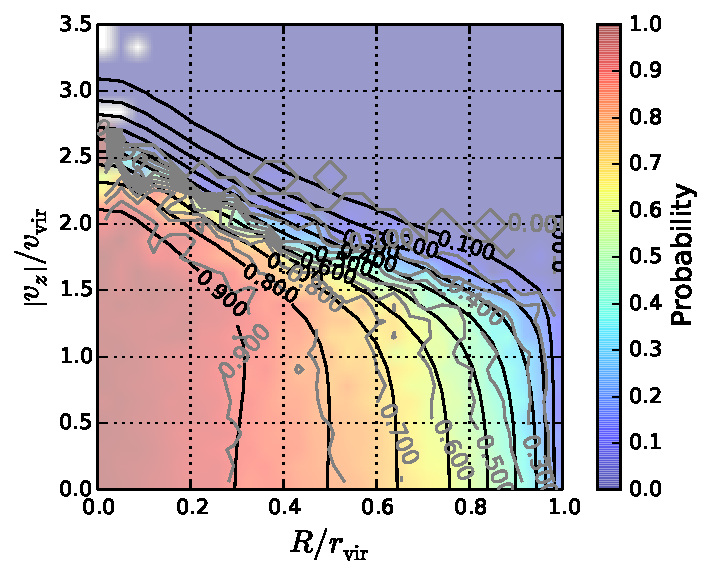
\includegraphics[width=0.6\linewidth]{figures/maggie/probabilities.pdf}
    \caption{The probability contours from the simulation of \citet{Borgani+01}
        and our model. In \emph{gray} the contours obtained with particles from
        the cosmological simulation, and in \emph{black} the theoretical
        expectation from \bartrefequation{gi_over_gh}. The color scale reflects
        the probability from the simulation. The theoretical probability agree
        with the cosmological simulation except for high velocities along the
        line-of-sight, in part explained by the lack of particles with such
        velocities, giving a bad constraint for the probability to be in the
        halo from the simulation.
\label{fig:probabilities}}
\end{figure}

\remark{%
    We can first think that the observed discrepancies in
    \bartreffigure{probabilities} are the consequence of a bad choice for the
    ratio $a/b$ (see \bartrefappendix{profiles}) or for the concentration, but
    changing this values doesn't reduce them. The contours for the simulation
    seem to show a cut-off in the line-of-sight velocity dispersion for high
    velocities, like if the distribution is truncated above a given velocity. A
    functional form with such a property is the generalization of the Gaussian
    called the $q$-Gaussian or Tsallis distribution. Assuming such a velocity
    distribution, the computation of the probability involves several
    integrals, which is CPU time consuming. Instead, we can fit a $q$-Gaussian
    on the line-of-sight velocity distribution from the simulation and
    incorporate it in the probability computation. But unfortunately, this
    doesn't solve the problem. It seems that the number of particles with high
    velocities is too low to correctly define the probability to be in the
    virial sphere of the halo, and to compare it to theoretical expectations.
    The velocity distribution isn't involved.
}

Here we assume that the density profile follow a NFW, since the dark matter
particles of the \citet{Borgani+04} simulation follow this distribution. But we
are interested in groups of galaxies and they must follow the same distribution
to apply our model. We used the galaxies from the output of the \citet{Guo+11}
semi-analytical code and checked that they follow a NFW density profile too.
But as expected, there is a bias between the galaxies and dark matter
particles. Indeed, if we fit the concentration of the NFW profile in
\citet{Guo+11} and compare it to the model of \citet{Maccio+08} obtained from
dark matter particles, we can see that the two functional are different. A
consequence is that the link between halo mass and concentration must be
adjusted for galaxies in our model. The difference between the two model of
concentration is shown in \bartreffigure{concentration_bias}.
%
\begin{figure}[ht]
    \centering
    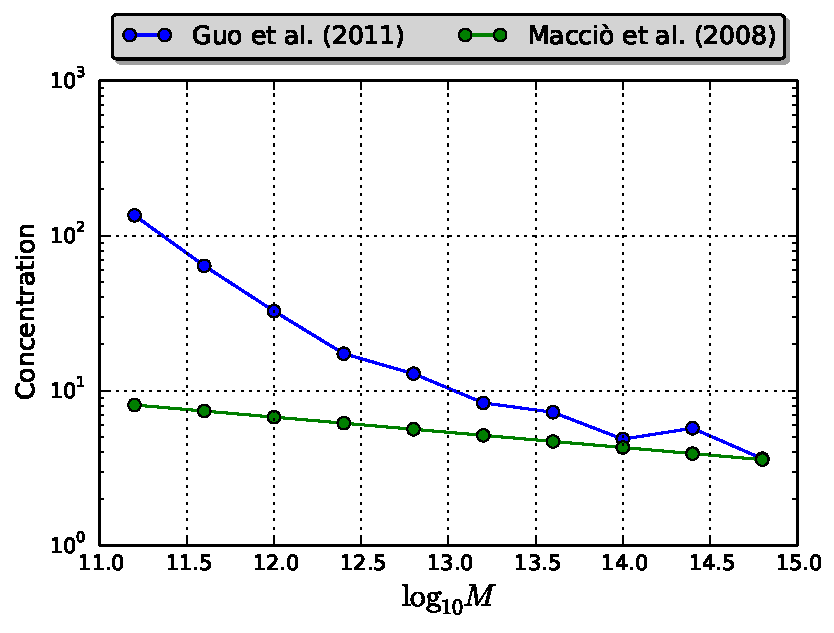
\includegraphics[width=0.8\linewidth]{figures/maggie/concentrations.pdf}
    \caption{The concentration in function of the halo mass for
        \citet{Maccio+08} in \emph{green} and fitted on the \citet{NFW+97}
        density profile of galaxies from \citet{Guo+11} with $M_r\leqslant-15$
        in \emph{blue}. The concentration of galaxies is slightly different
    from that of dark matter particles.\label{fig:concentration_bias}}
\end{figure}
%
But we note that the modulation of the concentration with the halo mass is
dependent of the cut-off in luminosity applied on the galaxy sample, making the
use of a specific density profile for galaxies inadequate. We checked the
influence of this choice on MAGGIE by comparing the performance with the
concentration from \citet{Guo+11} and from \citet{Maccio+08}. No noticeable
impact is observed in the completeness, reliability and fragmentation, except
on stellar masses and luminosities of groups but without being significant.

\section{Results on mock catalogue}
\label{sec:results_on_mock_catalogue}

\subsection{Description}
\label{sub:maggie_tests_description}

For tests we proceed as described in \citet{Yang+07, Duarte+14} and
\bartrefchapter{friends_of_friends_algorithm}. To link a selected group by the
algorithm in redshift space to the true halo in real space, we use the most
massive galaxy of the group. The true halo of a group is the true halo to which
the most massive galaxy in the selected group (referred as the central galaxy)
belongs to. With this link, we compute the completeness and reliability of
groups relatively to this halo in real space. We define statistics used to
quantify the performance of MAGGIE\@. The completeness $C$ is the fraction of
galaxies in the real space group recovered in the selected group. The
reliability $R$ is the fraction of galaxies in the selected group present in
the real space group. A primary group is defined as a selected group whose the
central galaxy match the central galaxy of the real space associated halo,
remaining groups are fragments. A complete and detailed description of the
statistics can be found in \citet{Duarte+14} and
\bartrefchapter{friends_of_friends_algorithm}.

The reliability in the case of MAGGIE is more complex since we use
probabilities for galaxies in groups. We let, with our definition, many
galaxies potentially belong to a given group. This artificially decreases
the reliability of a group because of the interlopers being systematically
considered group members with the previous definition. To take advantage of
our probabilities, let us give a new definition for the reliability. In
\citet{Duarte+14}, we wrote:
%
\begin{equation}
    R=\frac{T \cap E}{E}=\frac{\sum_{i\in T\cap E}}{\sum_{i\in E}}
\end{equation}
%
But many galaxies pertains to our group with this definition and so we
weight galaxies in the previous sum by their probabilities in order to have
a coherent definition of the reliability with our probabilistic
determination of groups. Our new definition in the case of a probabilistic
galaxy group algorithm as MAGGIE is:
%
\begin{equation}
    R=\frac{T \cap E}{E}=\frac{\sum_{i\in T\cap E} p_i}{\sum_{i\in E}p_i}
\end{equation}
%
For the completeness, since the probability doesn't introduce a bias in the
selection relatively to the real group, we keep the computation as described
in \citet{Duarte+14}, without weighting by probabilities.

Without probabilities, galaxies in groups form a complete partition of the
survey since groups can be seen as disjoints sets of the redshift space. But
with MAGGIE and probabilities, a galaxy can be in multiple groups so the
sets of groups are overlapping, and the \emph{dual} analysis done in
\citet{Duarte+14} for the merging of real space groups can't be correctly done.
This is because the central galaxy of a real space group can be potentially
belonging to several extracted group in the redshift space.

\subsection{Optimization}

MAGGIE depends on two probability thresholds: the first we call central
probability ($p_\mathrm{central}$) constraining the fragmentation of galaxy
groups by allowing galaxies to be the central galaxy of a potential galaxy
group, the second one the membership probability ($p_\mathrm{membership}$),
defining a threshold to consider or not a galaxy in a group for the computation
of its properties.

In fact, a galaxy is considered as possible central galaxy while looping
through ordered galaxies only if the galaxy has all its probabilities in its
other groups lower than the central probability threshold. For membership,
galaxies are ``affected'' to a group (i.e.\ they are assumed to have a
probability to be in this group) only if their probabilities are above the
threshold membership probability.

Checking the dependence of MAGGIE to these parameters is done in the same way
as we performed in \bartrefchapter{friends_of_friends_algorithm}. We computed
the mean completeness, reliability, fragmentation and merging, as well as the
quality factors we previously defined, for a range of threshold probabilities
$(p_\mathrm{central}, p_\mathrm{membership})\in{\left[10^{-15}, 0.4\right]}^2$.
Fortunately, results are not dependent of these thresholds. A small variation
is observed only for very high values of these probabilities (above 0.1).
Increasing these probabilities leads to relatively worst statistics, while
keeping them small is better, but without significant variations.

We selected the value 0.001 for both threshold probabilities. Since this value
is relatively small, we should notice that it is equivalent to defining the
membership in the virial cone constructed with the virial radius of the group.
The selection of background galaxies, far away in velocities, is avoided by
$p_\mathrm{membership}$, since with these value, when galaxies are beyond than
4--5 $v_\mathrm{vir}$ from the group, they are not considered. The same happens
for $p_\mathrm{central}$ where galaxies in membership can't create new groups.

When working with non-probabilistic algorithms, the set of galaxy groups is a
complete partition of the space formed by galaxies. In other words, groups are
non-overlapping and fragmentation is avoided naturally if the assignation is
done properly. But with probabilities and our method, removing these threshold
parameters, there is as many groups as galaxies. Putting thresholds to low
values make MAGGIE behaves like non-probabilistic algorithms, but keeping the
possibility to overlap some groups when things are very uncertain. But we
should note that we can't make them null or each galaxy group will be formed of
its entire virial cone. The introduction of threshold probabilities is a way to
make a ``compatibility'' between MAGGIE and its soft assignment and
non-probabilistic grouping algorithms and their hard assignments.

\subsection{Results}

The following tests result from the application of MAGGIE on the perfect mock
catalogue whose construction is described in \bartrefchapter{mock}. In this
case, we assume the halo mass function extracted from the Millennium-II
outputs, with a NFW density profile for galaxies identical to dark matter
particles in their halos. The influence of these assumptions will be developed
in \bartrefsection{maggie_discussions}.

We compare MAGGIE with the most popular galaxy group algorithm that is the
percolation algorithm (see \bartrefchapter{friends_of_friends_algorithm}). The
set of linking lengths used for the FoF is the one defined in~\cite{Duarte+14}
for an optimal FoF, close to the parameters used by~\cite{Robotham+11}, with
values of (\bperp, \bpar)$=(0.07, 1.1)$. This will let us see if the
introduction of Bayesian model improves the galaxy grouping compared to a
simple geometrical approach as FoF.

\subsubsection{Completeness and reliability}

\begin{figure}[t]
    \centering
    \begin{minipage}{0.49\linewidth}
        \subfloat[Catalogue 2]
        {%
            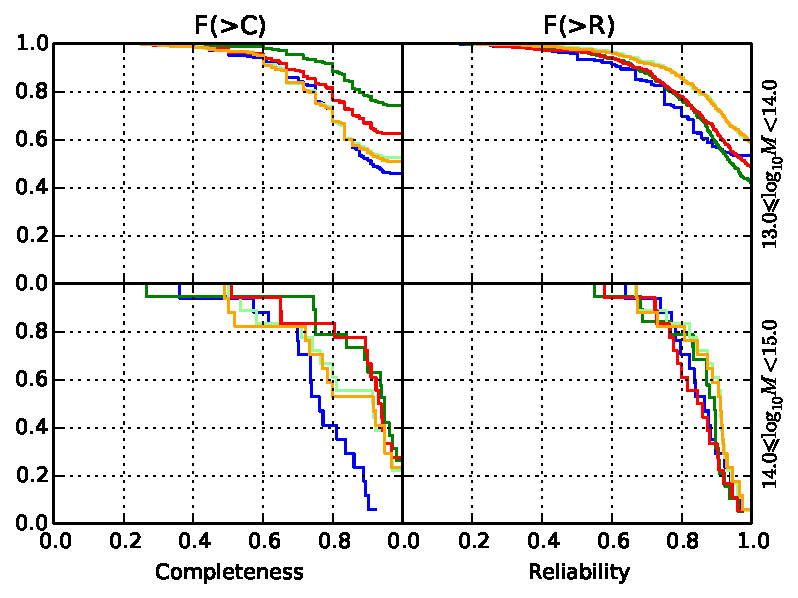
\includegraphics[width=\linewidth]{%
figures/maggie/article_fof_comparison_errors_CDF_completeness_reliability_1_article_C_R.pdf%
            }
        }
    \end{minipage}
    \begin{minipage}{0.49\linewidth}
        \subfloat[Catalogue 5]
        {%
            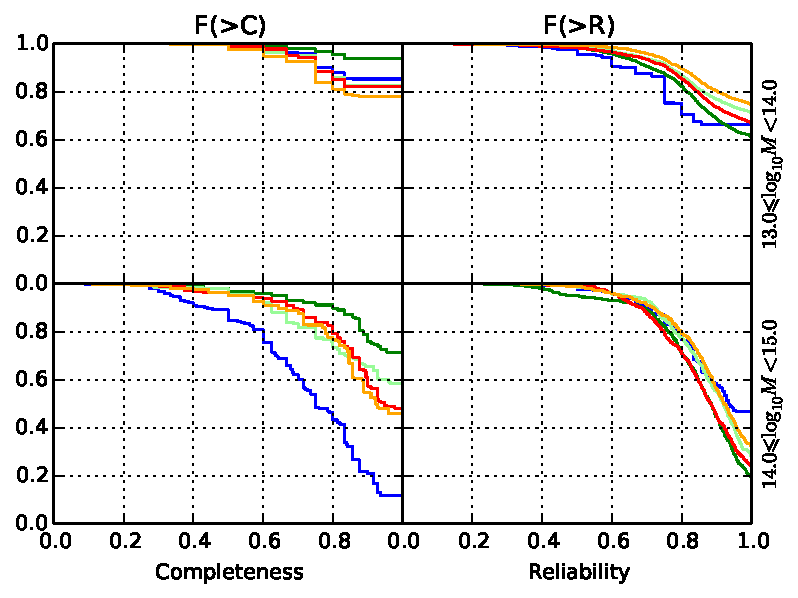
\includegraphics[width=\linewidth]{%
figures/maggie/article_fof_comparison_errors_CDF_completeness_reliability_5_article_C_R.pdf%
            }
        }
    \end{minipage}
    \caption{The cumulative distribution of the completeness $F(>C)$ and
        reliability $F(>R)$ for bins in true halo masses for two sub-samples of
        the mock catalogue. In \emph{dark green} MAGGIE, in \emph{blue} the
        optimal FoF. The \emph{light green} curve is also MAGGIE in the perfect
        case but using luminosities instead of stellar masses to do the
        abundance matching. The \emph{red} and \emph{gold} curves are
        respectively for MAGGIE with stellar masses and Gaussian errors
        ($\sigma=0.2$ dex) and MAGGIE with luminosities and Gaussian errors
        ($\sigma=0.04$ dex). Details for latter cases are in
        \bartrefsubsection{observational_errors}. Results are shown only for
    primary groups (i.e.\ groups that are not fragments of real space halos)
with the same filter as in
\bartrefchapter{friends_of_friends_algorithm}.\label{fig:comp_rel}}
\end{figure}

\bartreffigure{comp_rel} shows the cumulative distribution function of the
completeness $C$ and reliability $R$ as defined in
\bartrefsubsection{maggie_tests_description} for MAGGIE and the FoF algorithm.
Results are shown only for two doubly complete sub-samples (see
\bartrefchapter{mock}), the same as in
\bartrefchapter{friends_of_friends_algorithm}. Only two bins in halo mass are
used, and we use the true halo mass, i.e.\ the virial mass of the true halo
associated to the extracted group. MAGGIE (in dark green) shows a better
behaviour in completeness for all masses in both catalogues than FoF (in blue),
while the reliability is equivalent to the optimal FoF, except for high masses
for the bigger catalog.

\subsubsection{Group properties}

\begin{figure}[htb]
    \centering
    \begin{minipage}{\linewidth}
        \centering
        \subfloat[Comparison for group luminosities]
        {%
            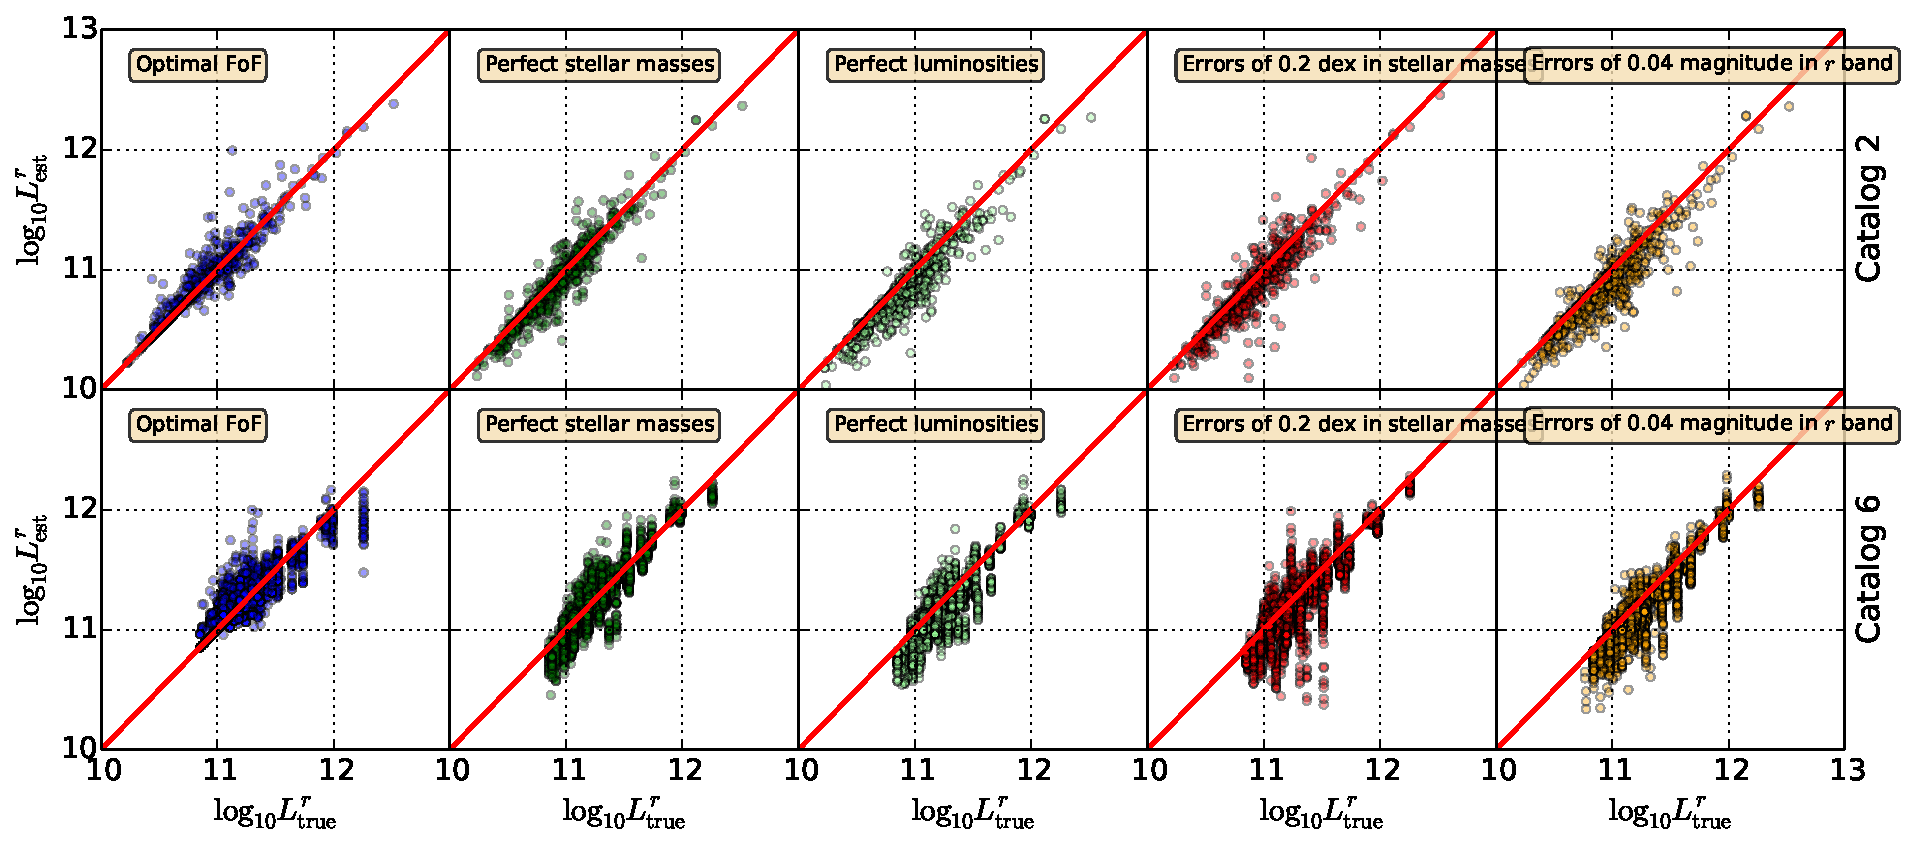
\includegraphics[width=0.8\linewidth]{%
figures/maggie/article_fof_comparison_errors_differences_luminosity.pdf%
            }
        }
    \end{minipage}
    \begin{minipage}{\linewidth}
        \centering
        \subfloat[Comparison for group stellar masses]
        {%
            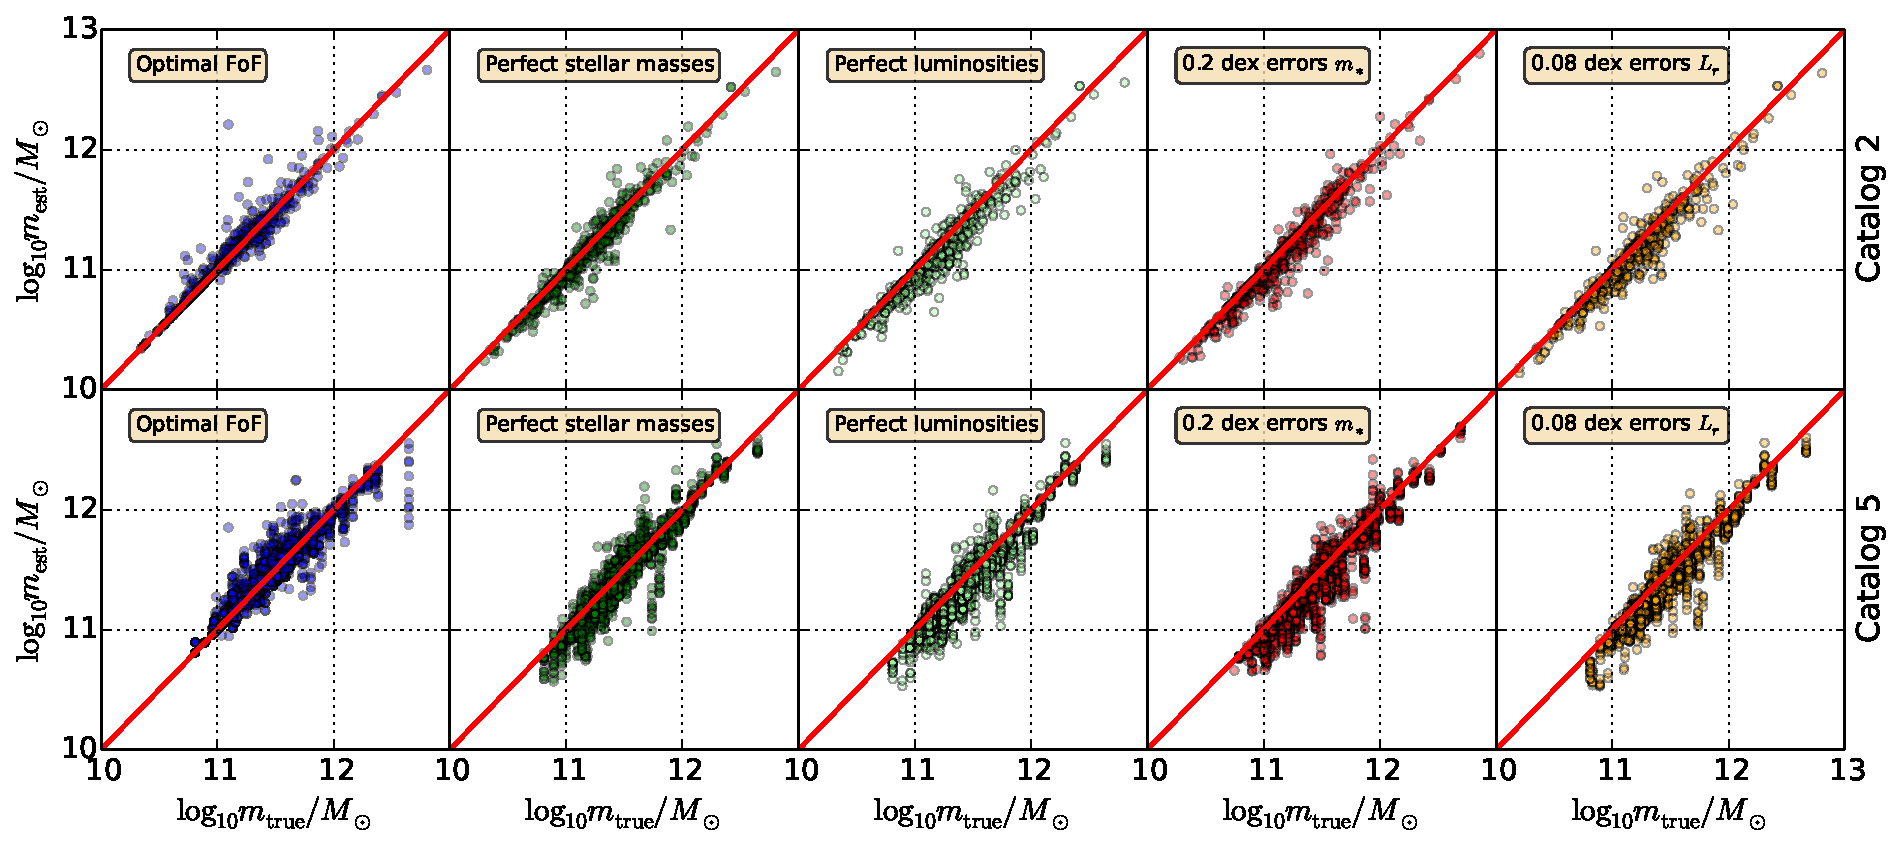
\includegraphics[width=0.8\linewidth]{%
figures/maggie/article_fof_comparison_errors_differences_stellarmass.pdf%
            }
        }
    \end{minipage}
    \captionof{figure}{Comparison of group luminosities in $r$ band and stellar
    masses with the real space for primary groups in catalogues 2 and
5.\label{fig:comparison}. Colors are the same as in \bartreffigure{comp_rel}.}
\end{figure}
%
\begin{figure}[htb]
    \centering
    \begin{minipage}{0.49\linewidth}
        \centering
        \subfloat[Bias and dispersion for luminosities]
        {%
            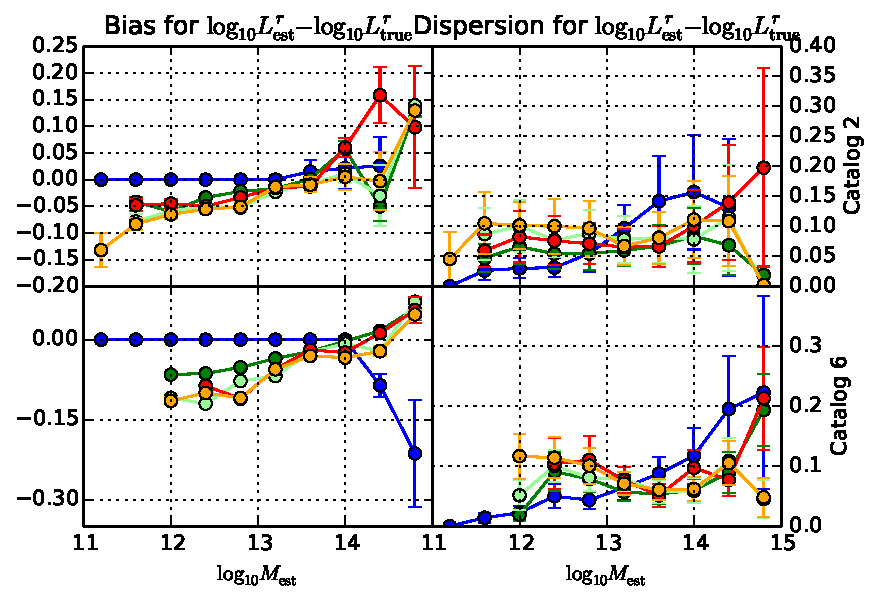
\includegraphics[width=\linewidth]{%
figures/maggie/article_fof_comparison_errors_bias_dispersion_luminosity.pdf%
            }
        }
    \end{minipage}
    \begin{minipage}{0.49\linewidth}
        \centering
        \subfloat[Bias and dispersion for stellar masses]
        {%
            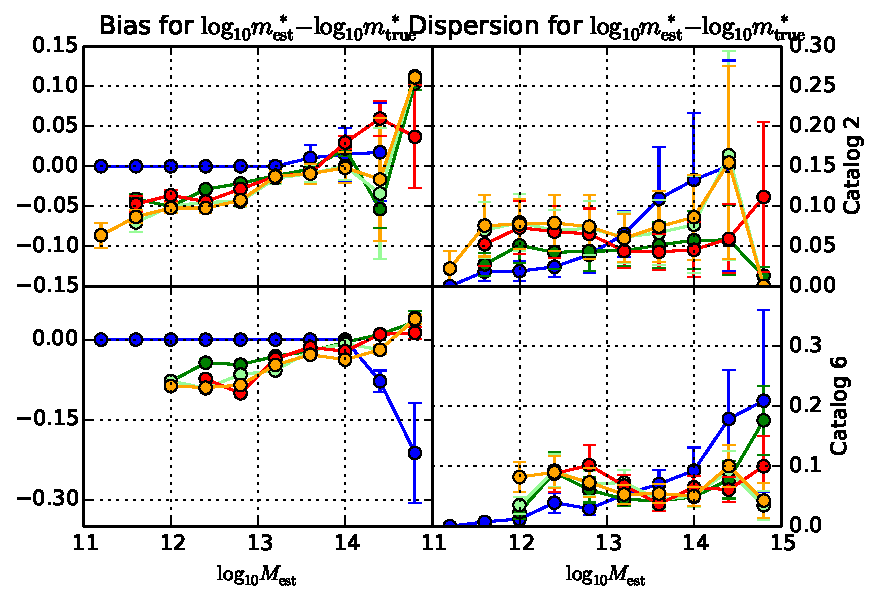
\includegraphics[width=\linewidth]{%
figures/maggie/article_fof_comparison_errors_bias_dispersion_stellarmass_bias.pdf%
            }
        }
    \end{minipage}
    \captionof{figure}{Bias and dispersion for group luminosities and stellar
    masses for catalogues 2 and 5. Colors are the same as in
\bartreffigure{comp_rel}.\label{fig:bias_disp}}
\end{figure}

We test the deduced stellar mass and luminosity of selected groups for each
algorithm. For non-probabilistic FoF, they are just the sum of the galaxy
contributions. But for MAGGIE, we use the computed probabilities inside the
group to weight the stellar mass and luminosity of each galaxy. If $X$ is the
property of the group, $x_i$ the property of the galaxy $i$ in the group with
the probability $p_i$:
%
\begin{equation}
    X = \sum_i p_i x_i
\end{equation}

In \bartreffigure{comparison} and \bartreffigure{bias_disp}, we compare the
true luminosity of groups (computed assuming a perfect selection of groups in
the sub-sample) with the luminosity computed with the galaxy membership of each
algorithm. In the bottom panel, we show the bias and the dispersion of the
difference between the true and estimated luminosities. These figures show the
same for stellar masses. The optimal FoF algorithm has a lower bias than MAGGIE
since we can't observe a trend of the bias with the true halo mass, while the
dispersion is better for MAGGIE at high masses thanks to the probability
weighting that reduces the effect of interlopers.

\subsubsection{Fragmentation}

Estimating the fraction of groups in the selection that are the result of the
fragmentation of a real group is important since an observer using a group
catalog can't distinguish the primary group from the other. In
\bartreffigure{fragments}, we show the fraction of fragmented groups (defined
as in \bartrefchapter{friends_of_friends_algorithm}) in function of the
estimated halo mass. This allows to see the expected fraction of fragmented
groups by an observer using a group catalog with only information on the
estimated halo mass.

MAGGIE shows a very better behaviour in the case of the fragmentation. The
observer can be always certain that a big halo isn't the result of the
fragmentation of a true halo. This is due to the combination of the abundance
matching that gives good estimations of virial masses and the ordered search
of groups from galaxy stellar masses. But the fragmentation increases with the
decreasing estimated virial mass, since with groups of few members, it is
easier to make a mistake in the selection of the central galaxy of the group.

\subsubsection{Virial masses}
%
\begin{figure}[htb]
    \centering
    \begin{minipage}{0.49\linewidth}
        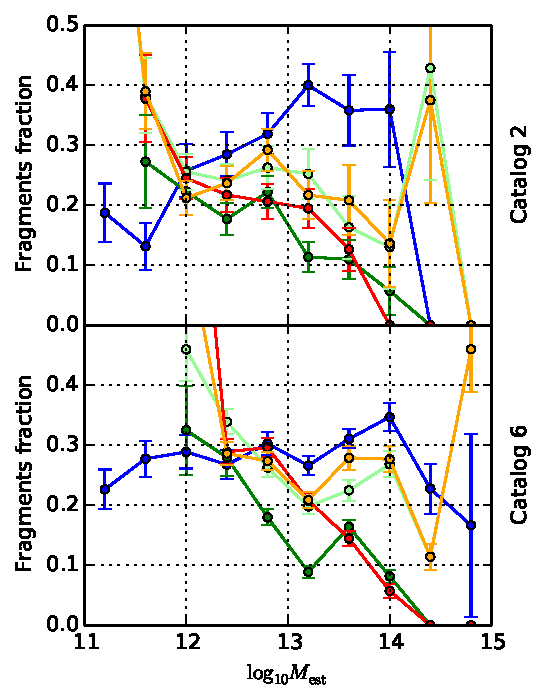
\includegraphics[width=\linewidth]{%
    figures/maggie/article_fof_comparison_errors_frag_fraction_fragments.pdf%
        }
        \captionof{figure}{The fraction of fragments in bins of estimated mass
        of extracted groups, for catalogues 2 and 5. Colors are the same as in
    \bartreffigure{comp_rel}.\label{fig:fragments}}
    \end{minipage}
    \begin{minipage}{0.49\linewidth}
        \centering
        \begin{minipage}{\linewidth}
            \subfloat[Comparison of virial masses]
            {%
                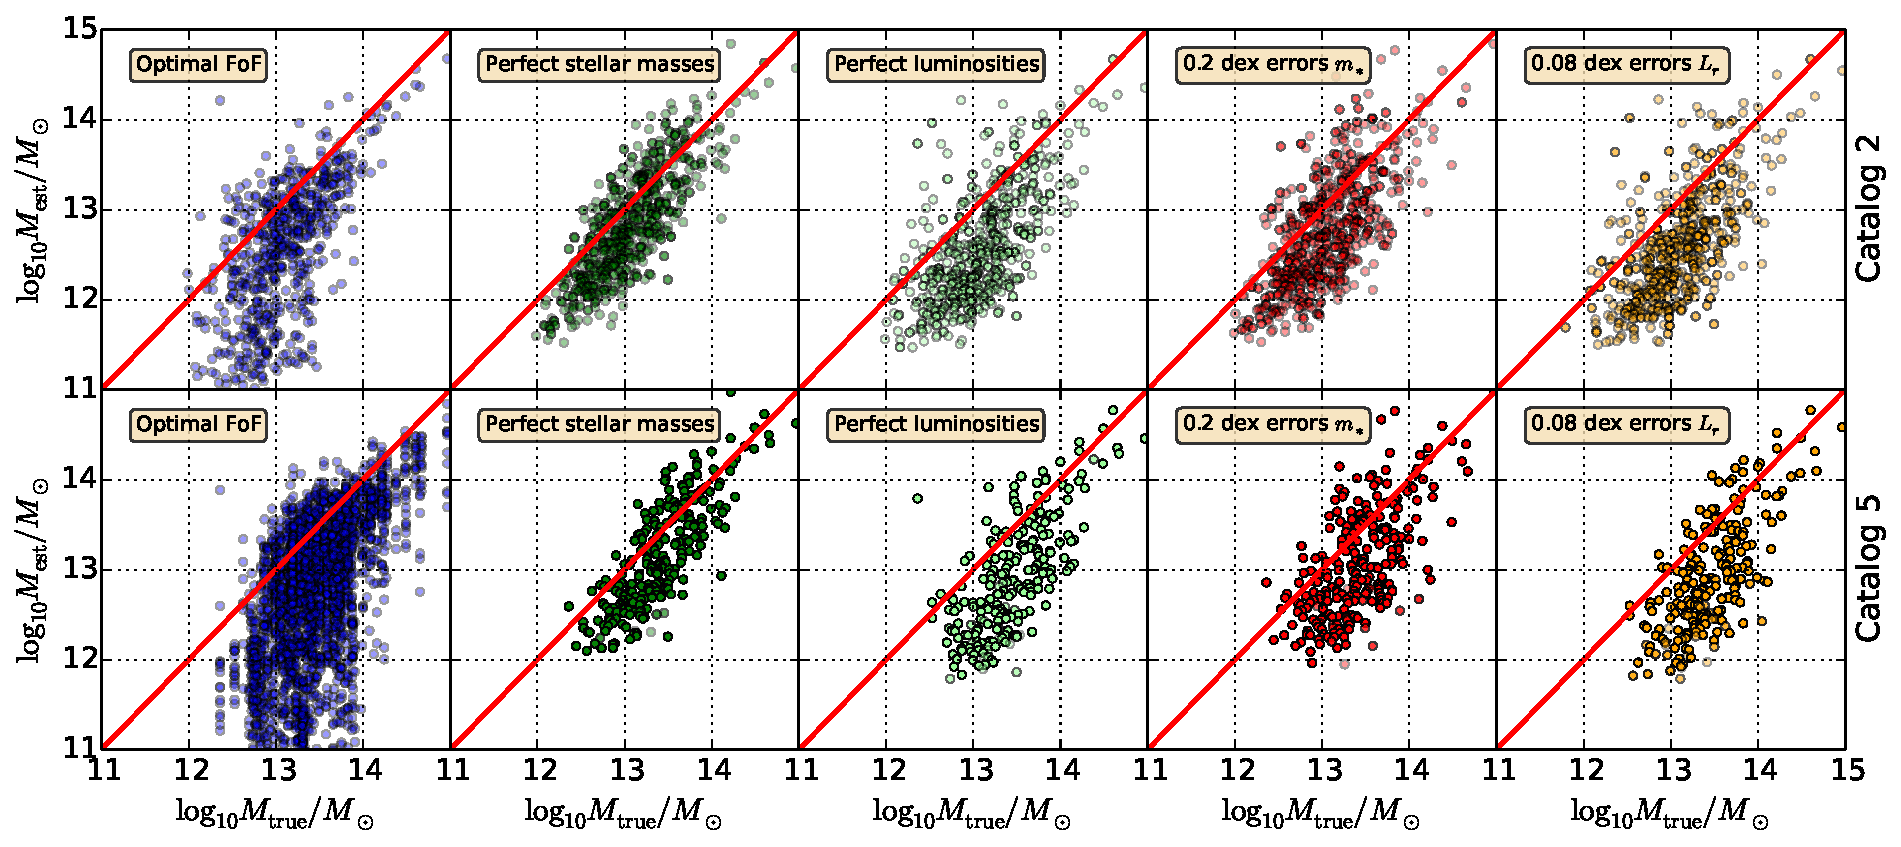
\includegraphics[width=\linewidth]{%
        figures/maggie/article_fof_comparison_errors_differences_halo_mass.pdf%
                }
            }
        \end{minipage}
        \begin{minipage}{\linewidth}
            \subfloat[Bias and dispersion for virial masses]
            {%
                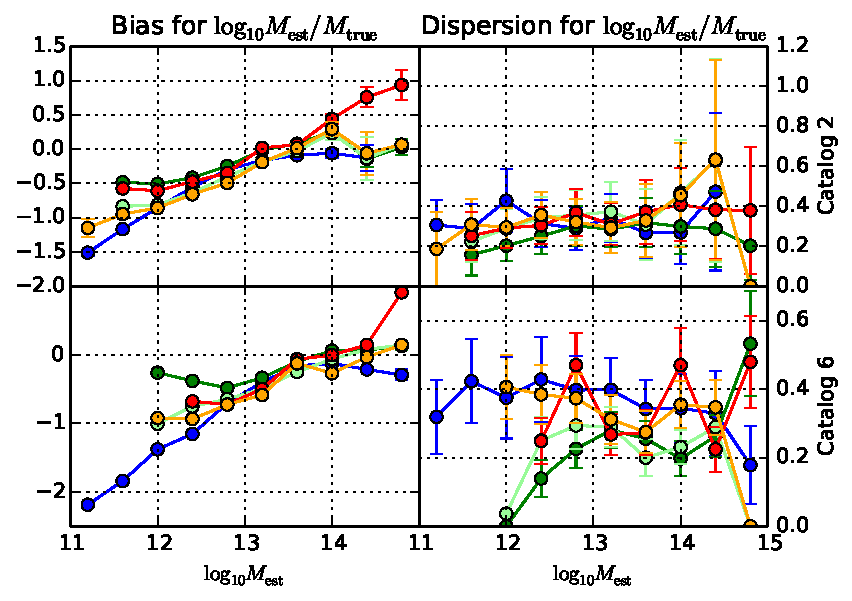
\includegraphics[width=\linewidth]{%
    figures/maggie/article_fof_comparison_errors_bias_dispersion_halo_mass.pdf%
                }
            }
        \end{minipage}
        \captionof{figure}{Comparison of the virial mass estimated by the
            galaxy group algorithms and the true masses obtained from the
            Millennium-II simulation, for catalogues 2 and 5. The top panel
            shows the comparison and the bottom panel bias and the dispersion
            of the logarithmic difference of masses. Colors are the same as in
        \bartreffigure{comp_rel}.\label{fig:bias_disp_virial_mass}}
    \end{minipage}
\end{figure}

In \bartreffigure{bias_disp_virial_mass}, we compare the estimation of the
virial mass by application of the virial theorem for FoF algorithm and by
abundance matching for MAGGIE\@. As we already discussed, the virial theorem
isn't very suitable in recovering the virial masses of groups when they have a
small mass (between $10^{12}$ and $10^{13}M_\odot$). We can't really see it in
the bias of the estimation between the two algorithms, but the difference is
pronounced in the dispersion where MAGGIE has a very good behaviour except for
high virial masses (around $10^{15}M_\odot$) as we expected because of the
choice of the relation for the abundance matching (see
\bartrefsubsection{hmf_test}). At this mass regime, the virial theorem improves
the estimation by the presence of more numerous galaxies putting less
uncertainties in the velocity dispersion of the group. Hence, a relative good
completeness in the group leads to a more precise virial mass.

\section{Discussions}
\label{sec:maggie_discussions}

A simple comparison of MAGGIE with the most popular and geometrical grouping
algorithm shows that MAGGIE is well adapted in recovering galaxy groups from
redshift space catalogues. Extracted global properties of groups are less
biased and catastrophic cases avoided by using probabilities as weights to
smooth the estimation. The membership inside these groups is better too since
the completeness shows that MAGGIE selects a large part of galaxies from the
real group, without polluting it by interlopers (as shown by the reliability).
Moreover, the importance of interlopers is reduced still by using
probabilities. The abundance matching technique is also a very good way to
contribute to this galaxy group extraction, since the virial mass estimation
relies only on group or galaxy properties, which are observables certainly
biased and uncertain, but with less importance than biased geometrical
informations (velocity dispersion, richness\ldots). On the contrary geometrical
informations perform well when the number of galaxies is important because
interlopers act as a small noise in the group membership, even with their
relative important presence at high halo masses for the FoF algorithm. Hence,
velocity dispersion and harmonic radius are not very biased and the virial
theorem becomes good.

This comparison is done in the case where the data on galaxies is perfect, in
the sense that there are no observational errors and we perfectly know the
various scaling relations used in our models. But the behaviour of MAGGIE is
unknown in the real situation of an observer, with a limited knowledge in these
models. In the following sections, we study the robustness of the performance
of MAGGIE under pertubations, i.e.\ in cases where we make some modifications
in the halo mass function, the galaxy luminosities and stellar masses\ldots, as
in studies of equilibriums.

\subsection{Prior halo mass --- central stellar mass relation}
\label{sub:prior_relation}

We tested the choice for the initial relation between the halo mass and the
central stellar mass of groups to see its effects on MAGGIE\@. We used the
relation from \citet{BCW+10} against a simple ratio relation with different
values for the ratio. Extracted groups are insensitive to this choice, if we
keep this choice with physical values. The iterative process corrects a bad
assumption in our initial guess.

\subsection{Influence of the halo mass function model}
\label{sub:hmf_test}

The estimation of the virial mass is an important aspect. Halo masses are
linked to the global environment of galaxies and a biased estimation will
affect observed trends of galaxy properties with the environment.

Our mass computation needs to be precise in the larger mass range possible, and
independent of polluted environment of groups by some interlopers. The
abundance matching technique seems to be a good way to estimate the virial mass
of galaxy group halos. In principle, it seems more biased than using the
luminosities or stellar masses of groups, but since the central galaxy in a
selected group is well recovered, this is a quantity less affected by
interlopers and so the halo mass estimation will be good enough. But since
there is a saturation of the relation between the halo mass and the central
stellar mass at high halo mass, we expect that the estimation will be poorer
for high masses than other methods.

The majority of the halo mass function described in the literature fit the FoF
mass of the halos instead of the spherical over-density mass, which is related
to the virial mass of the halo. Since we used the galaxy catalogue from
\citet{Guo+11} whose semi-analytical code was applied onto the Millennium-II
run, we fit the virial halo mass function directly on its output. We show it in
\bartreffigure{hmf} where we plot the FoF mass function (in red) and the virial
mass function (in black) for halos in the Millennium-II simulations at redshift
zero. Virial masses are lower than FoF masses so we don't use existing models
of halo mass functions displayed too on the figure. The way of computing such
halo mass function is described in \bartrefappendix{halo_mass_functions}.

\begin{figure}[htbp]
    \centering
    \begin{minipage}{0.49\linewidth}
        \subfloat[Catalogue 2]{%
            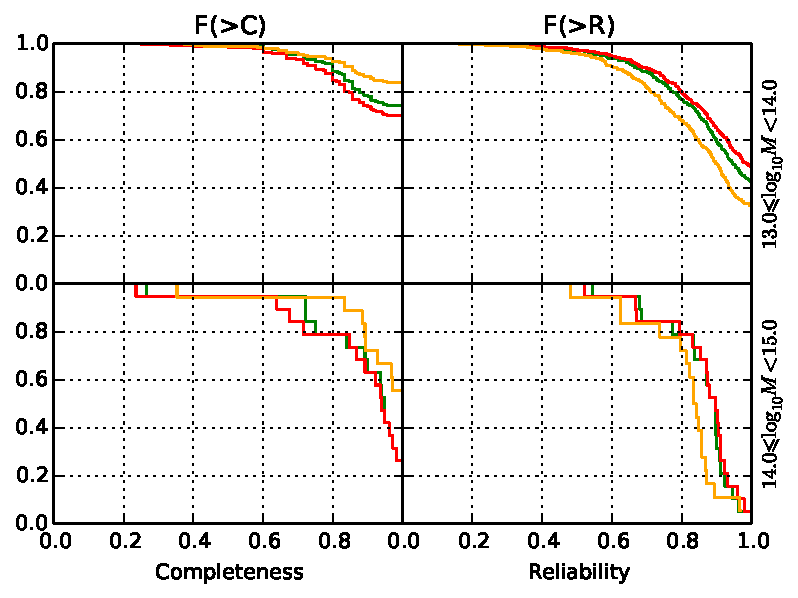
\includegraphics[width=\linewidth]{%
figures/maggie/msii_courtin_warren_CDF_completeness_reliability_1_article_C_R.pdf%
            }
        }
    \end{minipage}
    \begin{minipage}{0.49\linewidth}
        \subfloat[Catalogue 5]{%
            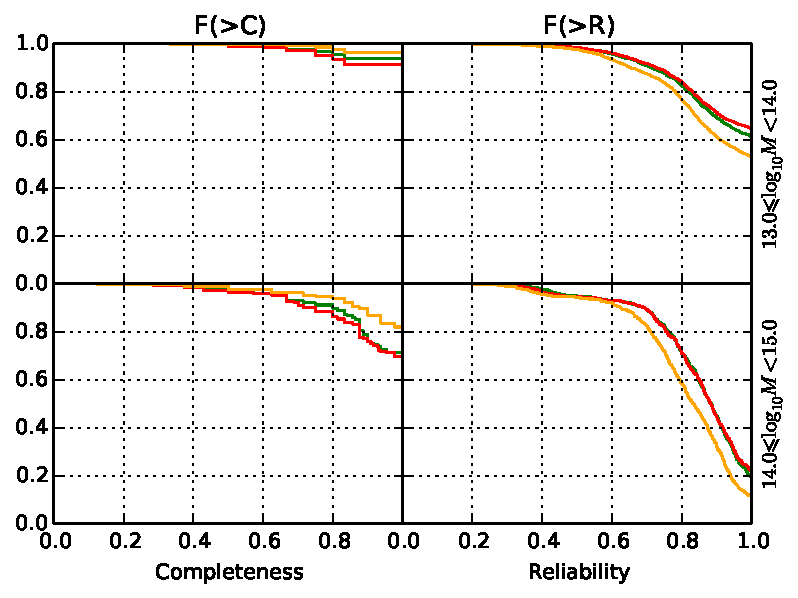
\includegraphics[width=\linewidth]{%
figures/maggie/msii_courtin_warren_CDF_completeness_reliability_5_article_C_R.pdf%
            }
        }
    \end{minipage}
    \captionof{figure}{The cumulative distribution function of the completeness
        and reliability for comparison of the perfect case of MAGGIE in
        \emph{green} with the halo mass function model of~\cite{Warren+06} in
        \emph{orange} and~\cite{Courtin+11} in \emph{red}. The filter applied
    on groups is the same as in \bartrefchapter{friends_of_friends_algorithm}.
A quite large error in the halo mass function seems to be not very dramatic in
the group membership.\label{fig:cdf_hmf}}
\end{figure}
%
\begin{figure}[htbp]
    \centering
    \begin{minipage}{0.49\linewidth}
        \subfloat[Group halo masses]{%
            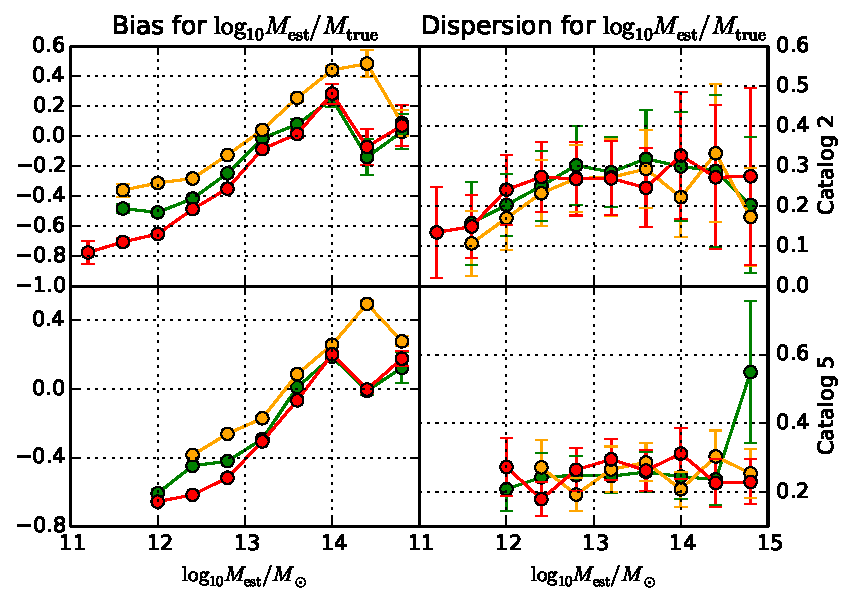
\includegraphics[width=\linewidth]{%
        figures/maggie/msii_courtin_warren_bias_dispersion_halo_mass.pdf%
            }
        }
    \end{minipage}
    \begin{minipage}{0.49\linewidth}
        \subfloat[Group stellar masses]{%
            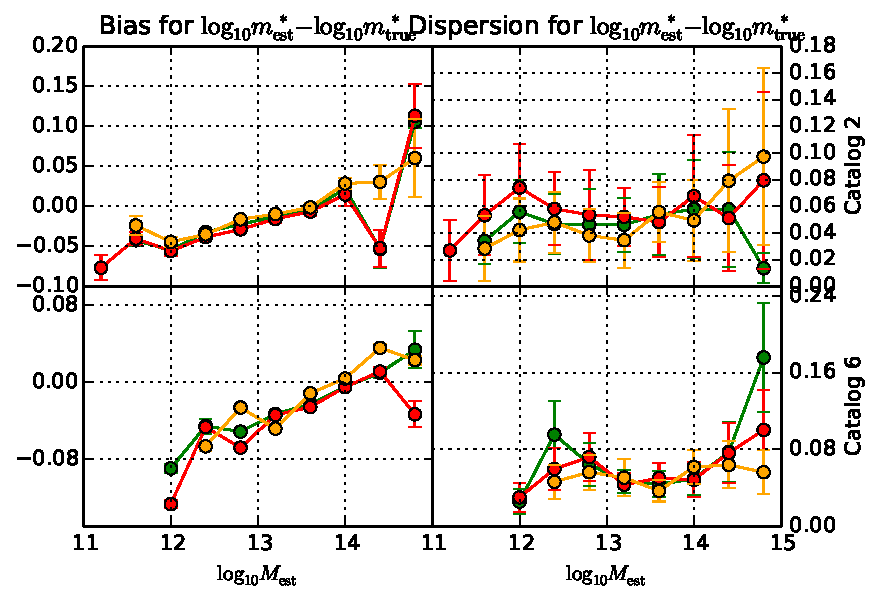
\includegraphics[width=\linewidth]{%
        figures/maggie/msii_courtin_warren_bias_dispersion_stellarmass.pdf%
            }
        }
    \end{minipage}
    \begin{minipage}{0.49\linewidth}
        \subfloat[Group luminosities]{%
            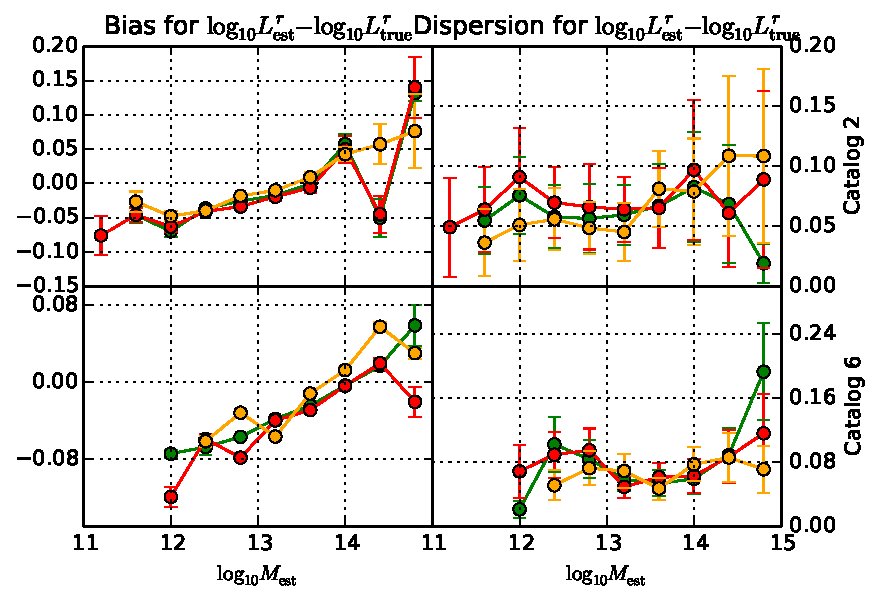
\includegraphics[width=\linewidth]{%
        figures/maggie/msii_courtin_warren_bias_dispersion_luminosity.pdf%
            }
        }
    \end{minipage}
    \captionof{figure}{Group properties compared to the perfect case of MAGGIE
    for both~\cite{Warren+06} and~\cite{Courtin+11} halo mass functions. Colors
and filter are the same as in \bartreffigure{cdf_hmf}. As seen in
\bartreffigure{cdf_hmf}, differences are not really
significant.\label{fig:bias_disp_hmf}}
\end{figure}

The robustness of MAGGIE against the choice of the halo mass function is
important because this choice will affect the completeness and reliability of
our selected groups and their properties too in a non obvious way. Indeed, the
halo mass function is a prior in MAGGIE and doesn't reflect necessary the
reality. We apply an equivalent of the perturbation method to test the
stability of MAGGIE under a bad choice of model. We used two halo mass
functions very different of the true one: \citet{Warren+06} and
\citet{Courtin+11}. Those models are fits of the FoF halo mass function from
different cosmological simulations. This is not the same as the virial mass but
ideal for perturbation test. The result of the application of MAGGIE with these
models is shown in \bartreffigure{cdf_hmf} and \bartreffigure{bias_disp_hmf}.

Comparisons are performed against the perfect case of MAGGIE (in green) with
the halo mass function directly fitted on the Millennium-II, perfect stellar
masses and luminosities for galaxies. In orange, halo mass function of
\citet{Warren+06} and in red, that one of \citet{Courtin+11}. The influence of
the halo mass function is very small on the completeness and reliability for
all catalogues and for group properties. The fragmentation is not shown but
behaves like in other plots, not affected by the choice of halo mass function.

\subsection{Influence of the cosmology}

Our problematic is still the same: as an observer, we don't know the real space
and its properties. So, we assume a given set of cosmological parameters. When
applying group finders on our mock catalog, we use the cosmology of the
simulation from which are constructed our mock. But in reality, we know those
parameters with a given uncertainty and we want to know their effects on the
group extraction.

To answer this question, we must know where the cosmology is relevant in the
algorithm. For example, when computing the projected radius of a galaxy at the
redshift of the group, we implicitly need to compute the luminosity distance
which is cosmology dependent. We assume in our case a flat Universe and in this
case, it is computed using just elliptic integrals
\citep{Liu+11,Eisenstein+97}. So cosmological parameters have an influence on
this distance, and in consequence, on the membership of galaxy groups.
Moreover, the halo mass function is dependent of the cosmology assumed by the
observer for many models and can affect the virial mass estimations. In our
case, the halo mass function is fitted on the real space data and its influence
can't be really measured. But we expect it has the same influence as a bad
choice for the halo mass function. We ran MAGGIE with the true cosmology (from
Millennium-II simulation) and two false cosmology with respect to our mock
catalog (Planck and WMAP9) to compare results. As expected, the importance of
the cosmology is low, of the order of statistical errors, as seen in
\bartreffigure{cdf_cosmology} and \bartreffigure{bias_disp_cosmology}.
%
\begin{figure}[htbp]
    \centering
    \begin{minipage}{\linewidth}
        \centering
        \begin{minipage}{0.49\linewidth}
            \subfloat[Catalogue 2]{%
                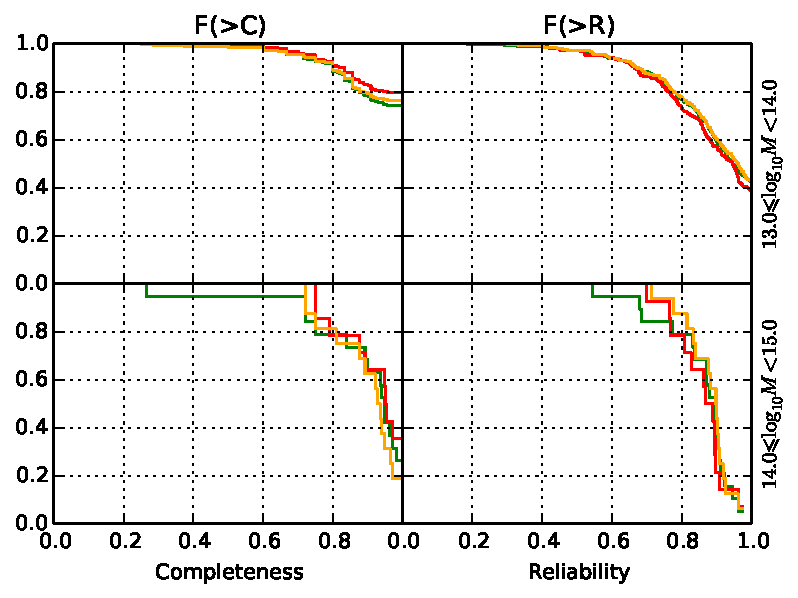
\includegraphics[width=\linewidth]{%
figures/maggie/planck_wmap9_CDF_completeness_reliability_1_article_C_R.pdf%
                }
            }
        \end{minipage}
        \begin{minipage}{0.49\linewidth}
            \subfloat[Catalogue 5]{%
                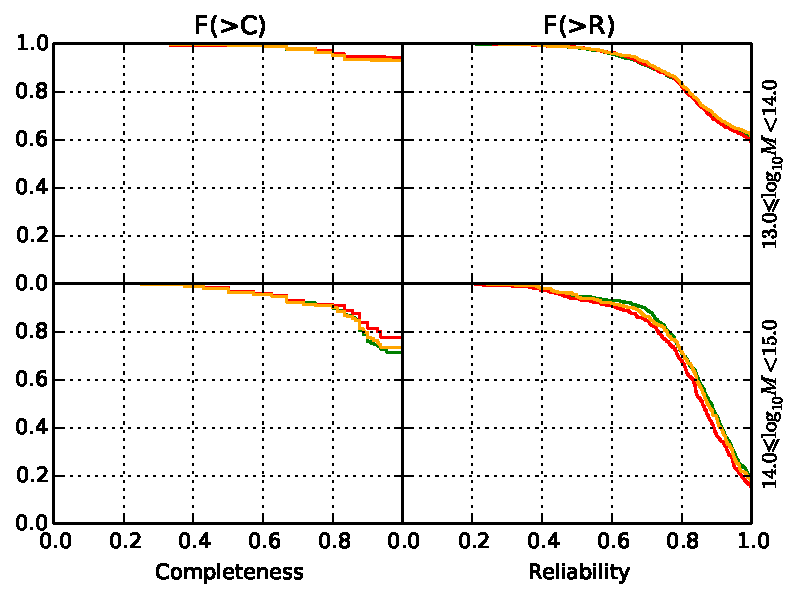
\includegraphics[width=\linewidth]{%
figures/maggie/planck_wmap9_CDF_completeness_reliability_5_article_C_R.pdf%
                }
            }
        \end{minipage}
        \captionof{figure}{Errors for the choice of the
        cosmology.\label{fig:cdf_cosmology}}
    \end{minipage}
    \begin{minipage}{\linewidth}
        \centering
        \begin{minipage}{0.49\linewidth}
            \subfloat[Group halo masses]{%
                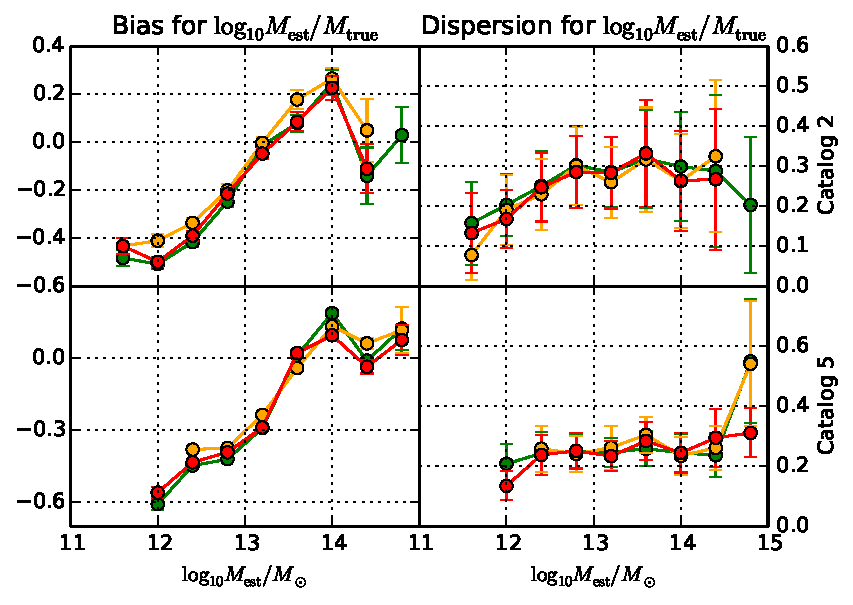
\includegraphics[width=\linewidth]{%
                figures/maggie/planck_wmap9_bias_dispersion_halo_mass.pdf%
                }
            }
        \end{minipage}
        \begin{minipage}{0.49\linewidth}
            \subfloat[Group stellar masses]{%
                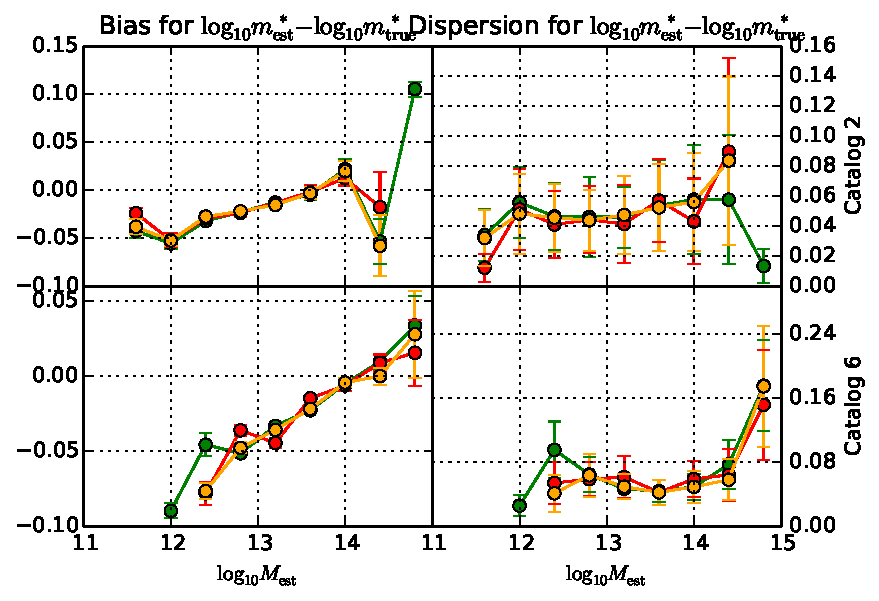
\includegraphics[width=\linewidth]{%
                figures/maggie/planck_wmap9_bias_dispersion_stellarmass.pdf%
                }
            }
        \end{minipage}
        \begin{minipage}{0.49\linewidth}
            \subfloat[Group luminosities]{%
                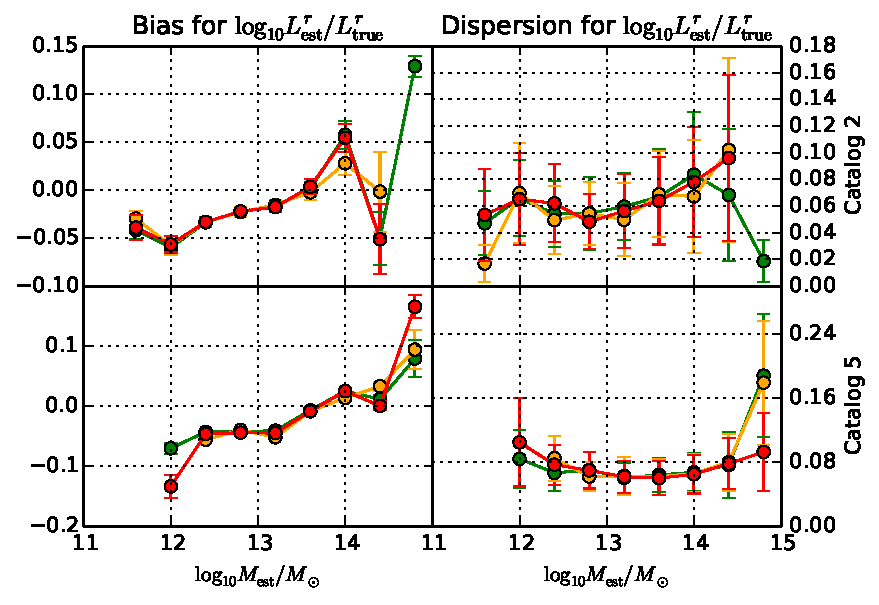
\includegraphics[width=\linewidth]{%
                figures/maggie/planck_wmap9_bias_dispersion_luminosity.pdf%
                }
            }
        \end{minipage}
        \caption{Errors for the choice of the
        cosmology.\label{fig:bias_disp_cosmology}}
    \end{minipage}
\end{figure}

\subsection{Influence of observational errors}
\label{sub:observational_errors}

Our way of sorting galaxies by mass uses our prior on the galaxy formation
scenario. Indeed, the stellar mass of the central galaxy of a dark matter halo
is correlated to its virial mass. But the relation is saturated at high halo
masses. So the intrinsic precision is affected by this choice. Moreover, the
estimation of stellar masses from the observations and spectrum is not very
precise and can significantly differ according to the way of computing it. We
show the differences between some models present in the SDSS data base, with
the bias and dispersion for each distribution, in \bartrefchapter{sdss}.

Typically, the errors in the estimation is roughly 0.2 dex. We introduce such
errors in the stellar masses of the mock catalogue to estimate the effect of
the bad estimation. We generated Gaussian errors without bias and dispersion of
0.2 dex. The application of MAGGIE on these galaxy mock catalogue is shown on
\bartreffigure{comp_rel}, \bartreffigure{comparison},
\bartreffigure{bias_disp}, \bartreffigure{fragments} and
\bartreffigure{bias_disp_virial_mass} in red color.

The effect of an error on stellar masses is quite catastrophic in the
completeness, compared to the case where the stellar masses are perfect (in
green). The percentage of groups with a perfect completeness decreases for
around 20 points for the catalogue 5 with a large volume, while this effect
isn't visible in the catalog 2 for high mass halos (since the volume of the
catalog is smaller, the number of high halo mass we expect to find is small too
and statistics poorer). The effect on the reliability is less important since
probabilities reduce the importance of interlopers introduced by the decrease
in completeness. In contrary, galaxy group properties are not very affected by
these errors in stellar masses, except for high halo masses. In this case, if
the most massive galaxy has not its mass well estimated, the estimation of the
halo mass is bad and probabilities can't ``correct'' this effect properly. This
is visible in \bartreffigure{bias_disp_virial_mass} where the bias in the
estimation of the halo mass is very important for high halo masses and the
dispersion is increased in all range of masses. In the other hand, the
fragmentation is increased for smaller halo masses, since with the decline in
completeness due to errors, high mass halos decompose into smaller parts at the
origin of the observed fragments.

So, errors in stellar masses are problematic and we should use an other tracer
for the halo mass as the central luminosity, which is less affected by
observational errors. Indeed, the principal sources of errors in the
computation of the absolute magnitude of a galaxy are the photometry, the
extinction, the K-correction, and the redshift through the distance modulus:
%
\begin{equation} \Delta M=\Delta m + \frac{5}{\ln{10}} \frac{\Delta
d_\mathrm{lum} \left(z\right)}{\Delta z} \frac{1}{d_\mathrm{lum}
\left(z\right)} + \Delta E + \Delta K\left(z\right) \end{equation}
%
$\Delta m$ for apparent magnitudes is of the order of $10^{-2}$ in the SDSS,
the second term is between $10^{-4}$ and $10^{-2}$ in the range of redshift
used for the catalogues. The K-correction $\Delta K$, if we follow the method
of \citet{Chilingarian+10}, is of the order of $10^{-2}$. There is the problem
of the extinction $\Delta E$ for which the precision can't be really estimated.
The Galactic extinction is estimated to 0.075, but the internal extinction of
galaxies is more imprecise and we provide a rough value of 0.1. Moreover,
peculiar velocities worst the situation since they contribute to the
computation of the distance modulus. But for non-nearby galaxies and globally,
the errors should be small.

The inclusion of the luminosity instead of stellar mass in the group extraction
process of MAGGIE is quite simple. The abundance matching between the virial
mass and the central stellar mass is replaced by an abundance matching between
the virial mass and the central luminosity. Intrinsically, using luminosities
instead of stellar masses in the inference of group virial masses is expected
to be less precise because the relation between the luminosity of the central
galaxy and the halo mass is more saturated for high mass groups. But the gain
is in the precision and the robustness relatively to the precision.

Comparing the perfect case of MAGGIE using galaxy luminosity (light green) to
the perfect case of stellar masses (dark green) shows, as expected, that the
completeness is worst for luminosities (the reliability is a little better
since the completeness has decreased). But group properties are not really
affected still by the use of probabilities to avoid bad membership. The
fragmentation is worst too since groups aren't entirely recovered (missing
galaxies are considered as belonging to fragment groups). For halo mass
estimations, the bias induced by using luminosities is comparable to the
perfect case of stellar masses. It is only in the dispersion that we observe
the counterparts, specifically for high halo masses, due to the uncertainties
introduced by the saturation in the relation between the central luminosity and
the virial mass in this range of halo masses. But it is approximately better
than using stellar masses with errors.

Adding errors following a Gaussian distribution without bias and a dispersion
of 0.08 dex on luminosities (0.2 magnitudes as we roughly deduced previously),
we compare it (light orange) to the perfect case of the luminosity. As
expected, introduced errors doesn't have a real impact, because the behaviour
of light orange and light green curves are roughly identical.

The negative point of using luminosities instead of stellar masses is that it
seems to contribute to the fragmentation of galaxy groups. But we should
discuss a little how we make a match between the real space and the observed
space. To say which galaxy is the central of a group in the real space, we
can't directly use the one given by~\cite{Guo+11} since in our mock catalogue,
there is a magnitude limit removing a large number of galaxies not sufficiently
luminous. The central is not necessarily the most luminous of the group and the
flux limit possibly hide us the central while the group is visible with help of
some of its galaxies. To define the central galaxy in real space, we use the
most massive in stellar mass of the group taking into account only galaxies
within the complete sample used. Without such a treatment, we could possibly
increase the fragmentation artificially by a lack of central galaxy in the
sample. With MAGGIE using luminosities, the central galaxy in extracted groups
has a strong chance to be the most luminous (not necessarily the most massive
in stellar mass) and the match with real space groups will frequently say that
the central galaxy of the extracted group is not the same as the true group,
resulting in a frequent fragmentation in tests. This is what we observe in the
results of MAGGIE with luminosities, an higher fragmentation than in the case
of stellar masses.

A possible conclusion is that observational errors are very important when
working with Bayesian galaxy group algorithms based on physical priors,
contrary to geometrical based algorithms where such kind of uncertainties don't
have an influence on their performances.

\subsection{Conclusion}
\label{sub:maggie_discussion_conclusion}

MAGGIE is a powerful galaxy group algorithm. The use of probabilities to
recover groups properties is very useful to avoid the problems inherent to the
inevitable interlopers present in the group membership. But when applied on
data with uncertainties, its performances are reduced compared to tests with a
perfect knowledge of the various needed observables. Although there are some
counterparts for MAGGIE on realistic data, we note that globally it performs
better than a FoF algorithm applied on perfect data. The extracted membership
is better than the FoF and the virial mass estimation by abundance matching
compared to the simple virial theorem used generally with the percolation
algorithm.

All of it make MAGGIE a suitable galaxy group tool to be applied on large
galaxy surveys such as the Sloan Digital Sky Survey (SDSS) and the Galaxy And
Mass Assembly (GAMA).

% \section{Application to SDSS}
% \label{sec:application_to_sdss}

% vim: set tw=79 ft=tex:


\bartchapterimage{heic0506a.jpg}
\chapter{SDSS-DR10 analysis}
\label{cha:sdss}
\bartthumb{heic0506a.png}
\minitoc%

\section{Introduction}

An application of MAGGIE on a real galaxy survey implies an analysis of the
galaxy sample. We must understand the various incompletenesses it suffers in
order to be able to correct them. Here we describe the analysis we performed on
the Sloan Digital Sky Survey, with the various problems we encountered.

\section{Analysis}

\subsection{Definitions}

In SDSS, stripes are bands of observations along great circles of the survey.
Each of them is composed of six parallel scanlines (of 13 arcmin wide) with
gaps of approximately the same width between them. Two stripes make a single
stripe of 2.5°. Each scanline include all the data (in $ugriz$), and is divided
in fields (that can overlap). So when accessing an observation at a given
position in the sky, we access a specific field. A given observation is
completely defined by its run number, the number of the camcol of the scanline
and by the field number.

The pipeline of the SDSS is applied for the objects extraction. They are
detected as pixel over-densities relative to the background. With this method,
multiple real and different objects can be seen as a single object. They are
linked by their pixels as galaxies using Friends-of-Friends algorithm. A
deblending algorithm is then applied to resolve child objects from their
parents (defined as the first detection). Then a resolve algorithm is applied
to extract the best object when multiple fields are overlapping.

There are numerous object flags that are useful to select well observed
galaxies. In the \texttt{PhotoObjAll} table, there is a \texttt{clean} for a
predefined selection of the most common good flags, which facilitates the
selection of galaxies.

There can be many problems with the photometry, with cases of bright galaxies
with sky levels not well estimated and missing faint galaxies for example. Most
of these known problems are corrected in the recent releases (DR9 and DR10).

Old releases worked with a spectrograph of 640 fibers, with collisions at
$55''$, while the new BOSS survey works with a 1000-fiber spectrograph but with a
greater collision size of $64''$. The coverage of the old releases should be
used for the new BOSS, so its better to use latest releases. Moreover, the
pipeline used for the spectrum had changed and improved along releases.

Following definitions given in the SDSS website, we can define two
coordinate systems in the survey.
%
\begin{description}
    \item[Great Circle:] This coordinates system is define with two angles
        $(\mu, \nu)$. Coordinates are relatives to one stripe so they can be
        used when working with galaxies inside a stripe region.

    \item[Survey Coordinates:] It's an other system similar to celestial
        coordinates but ``centred'' on the contiguous block of galaxies  of
        the survey. Coordinates are written $(\lambda, \eta)$. The range of
        these coordinates is: $-\cfrac{\pi}{2}<\eta<\cfrac{\pi}{2}$ and
        $-\pi<\lambda<\pi$.
\end{description}
%
We will work only with survey coordinates as they allow us to easily define
a mask for the SDSS\@. The celestial coordinates and survey coordinates are
the same system of coordinates, except that one is a particular rotation of
the other. The relations between the two systems are:

\subsubsection{Survey coordinates to celestial coordinates}

\begin{eqnarray}
    \delta &=&
        \arcsin\left(\cos\lambda\sin\left(\eta+\delta_0\right)\right)
        \nonumber\\
    \alpha &=&
        \mathrm{atan2}
        \left(\sin\lambda,\cos\lambda\cos\left(\eta+\delta_0\right)\right)+
        \alpha_0\nonumber\\
\end{eqnarray}
%
with ${\left(\alpha_0,\delta_0\right)}_{\left(\alpha,\delta\right)}=
{\left(185°,32.5°\right)}_{\left(\alpha,\delta\right)}=
{\left(0,0\right)}_{\left(\lambda, \eta\right)}$.

\subsubsection{Celestial coordinates to survey coordinates}

The inverse transformation is:
%
\begin{eqnarray} \eta &=& \mathrm{atan2}
\left(\sin\delta,\cos\delta\cos\left(\alpha-\alpha_0\right)\right)-
\delta_0\nonumber\\ \lambda &=&
\arcsin\left(\cos\delta\sin\left(\alpha-\alpha_0\right)\right) \nonumber\\
\end{eqnarray}
%
with ${\left(\alpha_0,\delta_0\right)}_{\left(\alpha,\delta\right)}=
{\left(185°,32.5°\right)}_{\left(\alpha,\delta\right)}=
{\left(0,0\right)}_{\left(\lambda,\eta\right)}$. Periodic conditions must be
applied to angles found by the latter equation:
%
\begin{equation} \begin{cases} \eta\rightarrow\eta+180° \;
    \lambda\rightarrow180°-\lambda& \mbox{if}\;\eta<-90°\;\mbox{or}\;
    \eta>90°\\ \eta\rightarrow\eta-360° & \mbox{if}\;\eta>180°\\
    \lambda\rightarrow\lambda-360° & \mbox{if}\;\lambda>180°\\ \end{cases}
\end{equation}
%
\subsubsection{Stripe number}
%
Stripes have a constant width of 2.5° along the $\eta$ coordinate. So, stripe
number $n$ of a galaxy with $\eta$ coordinate is:
%
\begin{equation} n = \mathrm{floor}\left(\cfrac{\eta+58.75°}{2.5°}\right)
\end{equation}
%
\subsection{Galaxy selection}
%
Many tables in the SDSS save galaxies and other objects properties extracted
from images of the survey. These tables are the results of different selections
in objects extracted in images. When crossing objects between images of the
survey that overlap, there are some differences in positions for the same
object. So there are possibilities that an object is observed twice or more. In
many of those tables, there is no object duplicated.

In the SDSS database, the \texttt{Galaxy} view is a selection from the
\texttt{PhotoPrimary} for objects flagged as \emph{galaxy}, with
\texttt{type}=3. The \texttt{Galaxy} view contains the photometric parameters
(no redshifts or spectroscopic parameters) measured for resolved primary
objects. But we have other useful informations to link with tables that give us
photometric and spectroscopic redshifts. There is the \texttt{specobjid} entry
to link with spectroscopic redshifts in the table \texttt{SpecObj} which
doesn't contain duplicates (it's a clean table of \texttt{SpecObjAll} with
clean redshifts). If \texttt{specobjid=0}, the galaxy doesn't have a
spectroscopic redshift (the galaxy wasn't spectroscoped). The \texttt{objid}
allows to link to the \texttt{Photoz} table which contains all photometric
redshifts for galaxies in the \texttt{Galaxy} table. Estimation is based on a
robust fit on spectroscopically observed objects with similar colors and
inclination angle. There is also the \texttt{PhotozRF} where estimates are
based on the Random Forest technique. Galaxies in the SDSS are limited to
$m_r<17.77$ and a given surface brightness. So we need to apply the same flux
limitations when selecting galaxies on the \texttt{Galaxy} table. A possible
\texttt{SQL} query for selecting galaxies in this table and link them with
redshift tables is for spectroscoped galaxies:
%
\begin{listing}[H]
    \begin{minted}[bgcolor=griscode, linenos]{sql}
SELECT G.ra, G.dec, G.petroMag_u, G.petroMag_g, G.petroMag_r,
G.petroMag_i, G.petroMag_z, G.specobjid, G.objid, Z.z, Z.Zerr
FROM Galaxy AS G
JOIN SpecObj AS Z ON Z.specobjid=G.specobjid
WHERE G.specobjid!=0
AND G.petroMag_r-G.extinction_r<17.77
    \end{minted}
\end{listing}
%
and for galaxies which couldn't be spectroscoped:
%
\begin{listing}[H]
    \begin{minted}[bgcolor=griscode, linenos]{sql}
SELECT G.ra, G.dec, G.petroMag_u, G.petroMag_g, G.petroMag_r,
G.petroMag_i, G.petroMag_z, G.specobjid, G.objid, Z.z, Z.Zerr
FROM Galaxy AS G, Photoz AS Z
WHERE G.specobjid=0
AND G.objid=Z.objid
AND G.petroMag_r-G.extinction_r<17.77
    \end{minted}
\end{listing}

Stripe limits are given in the table \texttt{StripeDefs} but they represent
the limits that were planned at the beginning of the survey, not the actually
observed limits.

Some planned regions aren't still observed, so we need to define other limits
in $\lambda$ coordinates for incomplete stripes. We find, by hand, the new
limits of stripes which contains spectroscoped galaxies. Now, the survey mask
is like in \bartreffigure{sdss}. We will consider just galaxies in this mask in
order to find groups in the SDSS\@.
%
\begin{figure}[ht] \centering
    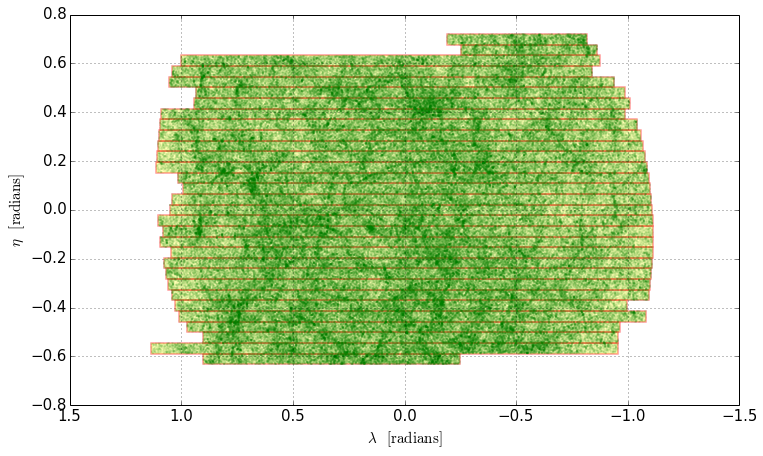
\includegraphics[width=\linewidth]{figures/sdss/sdss.png}
    \caption{Galaxies in the SDSS DR10 with stripes limits defined by hand. The
    red lines limits of the stripes make the SDSS mask used to identify
edges.\label{fig:sdss}}
\end{figure}

\subsubsection{Flags in the SDSS}

Galaxy photometry can have some troubles in the SDSS\@. In the general case,
those objects are flagged with \texttt{clean} property which indicates by 1
that the photometry is OK and by 0 when there is a problem. Details of the
problems are in the bit flag. But for groups, we need to select all galaxies,
even if they are not clean, or our groups will suffer incompleteness in their
membership and their physical properties such as luminosity, stellar mass\ldots
will be biased.

However, we have to take into account the error on the redshift estimation
using \texttt{zErr}. For photometric redshifts, if \texttt{zErr} is too high,
we can use \texttt{nnAvgZ}, which is the average redshift of galaxies in the
neighbourhood of the considered galaxy. It can be better if the photometric
redshift is strongly different from its value.

\texttt{SpecObjAll} contains duplicates and bad data. But \texttt{SpecObj}
contains just clean spectra. The field \texttt{zWarning} can be used to decide
if we keep a redshift or not.

\subsection{Fibre collision estimation}

We need a sample of galaxies for which we can easily characterize borders and
where all galaxies are present given the flux limit of the survey. But there is
the problem of missing galaxies due to fibre collisions. But our algorithm is
tested on a ``perfect'' mock catalogue. In order to know the behaviour of the
algorithm with these problematic galaxies, we need to implement the effect of
fibre collisions in our mock catalogue.

In the SDSS, galaxy spectra are obtained on fibers using a plate of 1.5°
diameter. But on the plate, the number of fibres is limited. Moreover, each
portion of the sky can't be spectroscoped multiple times, because the SDSS
had to cover a predefined portion of the sky in a fixed number of years.
Although spectroscopic runs may overlap, there are galaxies that can't be
spectroscoped. Indeed, while fibres collect spectra in a $3''$ diameter field,
their coatings prevent two fibres of lying close than $55''$ from one another.
When galaxies are closer than this distance, one (or more) of those galaxies
aren't spectroscoped. We can see this fibre collision effect in
\bartreffigure{plane}, where we have taken the nearest neighbour of a galaxy on
the celestial sphere, and determined the differences in angular positions and
redshift between the two galaxies. As expected, the number of galaxies that are
closer than $55''$ is much less than what would be extrapolated from greater
separations. There are still some galaxies because the overlapping of runs
allows to observe galaxy spectra below this limit.

\begin{figure}[ht] \centering
    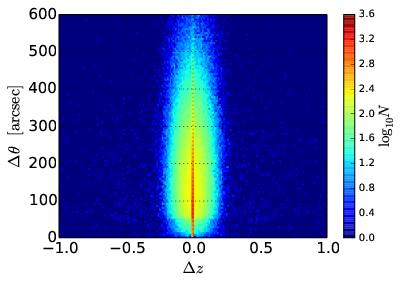
\includegraphics[width=0.6\linewidth]{figures/sdss/plane.png}
    \caption{\footnotesize{}Distribution of spectroscoped galaxies in the SDSS
    DR8 in angular size and redshift differences with the nearest neighbour
galaxy.\label{fig:plane}} \end{figure}
%
Nevertheless, the dense regions with more than one galaxy per $55''$ diameter
circle are partially incomplete in the SDSS spectroscopic sample.

We tried to implement this selection effect in our mock catalogue. For this, we
computed the local density in the field, taking all galaxies (spectroscoped or
not) in the neighbourhood of 1.5° around each galaxy, and at the same time, we
determine the fraction of galaxies that do not have a spectroscopic redshift,
to see the relation between spectroscopic completeness and photometric galaxy
number density. We expect to deduce a relation between the density field and
the fraction of fibre collisions. In the mock catalogue, we compute the same
density field and we apply the spectroscopic completeness relation estimated in
the SDSS sample to the mock. We have to remove galaxies that are close to
survey edges, because otherwise, there are missing galaxies and the
spectroscopic completeness will be affected. Edge galaxies are those lying
closer than 1.5 deg from the survey edges, which we measure in practice by
generating XXX random points within a circle of 1.5 deg radius around each
galaxy.

\remark{%
    We can generate samples of points at an angular distance $d$ to a point at
    position $(\alpha_0,\delta_0)$ using formulas of the spherical triangle.
    If we define a triangle by the pole, the point $(\alpha_0,\delta_0)$ and
    the point whose we want coordinates $(\alpha,\delta)$, we can write the
    following relations using the spherical triangle and its dual:
    %
    \begin{eqnarray}
        \sin\delta&=&\sin\delta_0\cos d + \cos\delta_0\sin d
        \cot\gamma\nonumber\\
        \sin\delta_0\cos\gamma&=&\cos\delta_0\cot{d}-\sin\gamma\cot\left(\alpha-\alpha_0\right)\nonumber\\
    \end{eqnarray}
    %
    where $\gamma$ is like a polar angle, which have all the values between 0
    and $2\pi$. We can rewrite:
    %
    \begin{eqnarray}
        \delta &=&
        \arcsin\left(\sin\delta_0\cos d + \cos\delta_0\sin d\cos\gamma\right)\nonumber\\
        \alpha-\alpha_0 &=& \arctan\left(\cfrac{\sin\gamma}{\cos\delta_0\cot{d}-\sin\delta_0\cos\gamma}\right)\nonumber\\
    \end{eqnarray}
    %
    There are problems at poles. For a $\gamma_0$ limit, angles can't be
    recovered with above formulas. Indeed, the problem appears when
    $\tan\Delta\alpha\rightarrow\infty$. So:
    %
    \begin{equation}
        \cos\delta_0\cot d -\cos\gamma_0\sin\delta_0 = 0
    \end{equation}
    %
    implying:
    %
    \begin{equation}
        \cos\gamma_0=\cfrac{1}{\tan d\tan\delta_0}
    \end{equation}
    %
    So to handle these limit cases, we summarize the correction for the
    differences in right ascensions by:
    %
    \begin{eqnarray}
        \Delta\alpha \rightarrow \Delta\alpha+\pi &\mathrm{if}&
        \mathrm{sign}\left(\delta_0\right)\cos\gamma \geqslant
        \mathrm{sign}\left(\delta_0\right)\cos\gamma_0\nonumber\\
    \end{eqnarray}

    Another way to draw circles on the sphere is to consider the point for
    which we want to know celestial coordinates around a given angular distance
    as the pole of a new coordinate system. In this system, points at a given
    distance of our central point are just points with $\pi/2-\delta$ and
    $\alpha$ running between 0 and $2\pi$. We now can determine cartesian
    coordinates of those points in this system and apply a rotation to go from
    the ``real'' system to the system where the central point is the pole. This
    can be easily done if we know the axis of rotation and the angle using
    quaternions, which is numerically more efficient than Euler angles.
}
%
We didn't see the trend we expected with the density field, so we thought that
it can be due to the large area in which we compute the fraction of
spectroscoped galaxies and we ran the same with a radius of 0.3°, but without
success too.

Moreover, including photometric redshifts in the mock catalogue and in MAGGIE
is very complex. For example, we measured the bias and dispersion of the
distribution of differences between spectroscoped and photometric redshifts in
the SDSS\@. \bartreffigure{redshift_difference} shows that while the dispersion
remains roughly constant, the bias increases with the spectroscoped redshift.
So some effects are not still under control when computing photometric
redshifts, and we should avoid their use in galaxy group algorithms when
possible. In the case of surveys where spectroscopic redshifts are not
available, the photometric redshifts should be as clean as possible.

\begin{figure}[hp]
    \begin{minipage}{\linewidth}
        \centering
        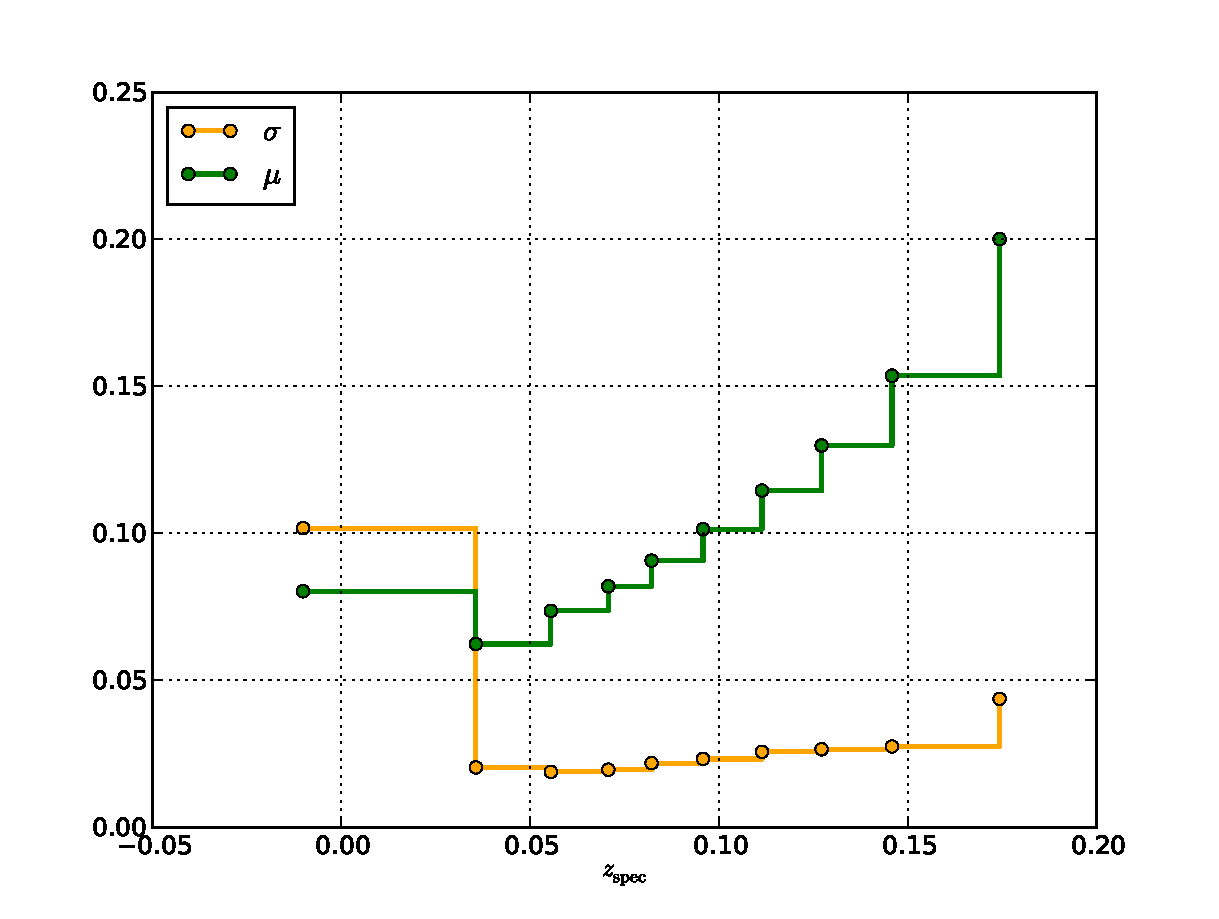
\includegraphics[height=0.4\textheight]{%
            figures/sdss/redshift_difference.pdf%
        }
        \captionof{figure}{Bias ($\mu$) and scatter ($\sigma$) of
        $z_\mathrm{phot} - z_\mathrm{spec}$.\label{fig:redshift_difference}}
    \end{minipage}
    \begin{minipage}{\linewidth}
        \centering
        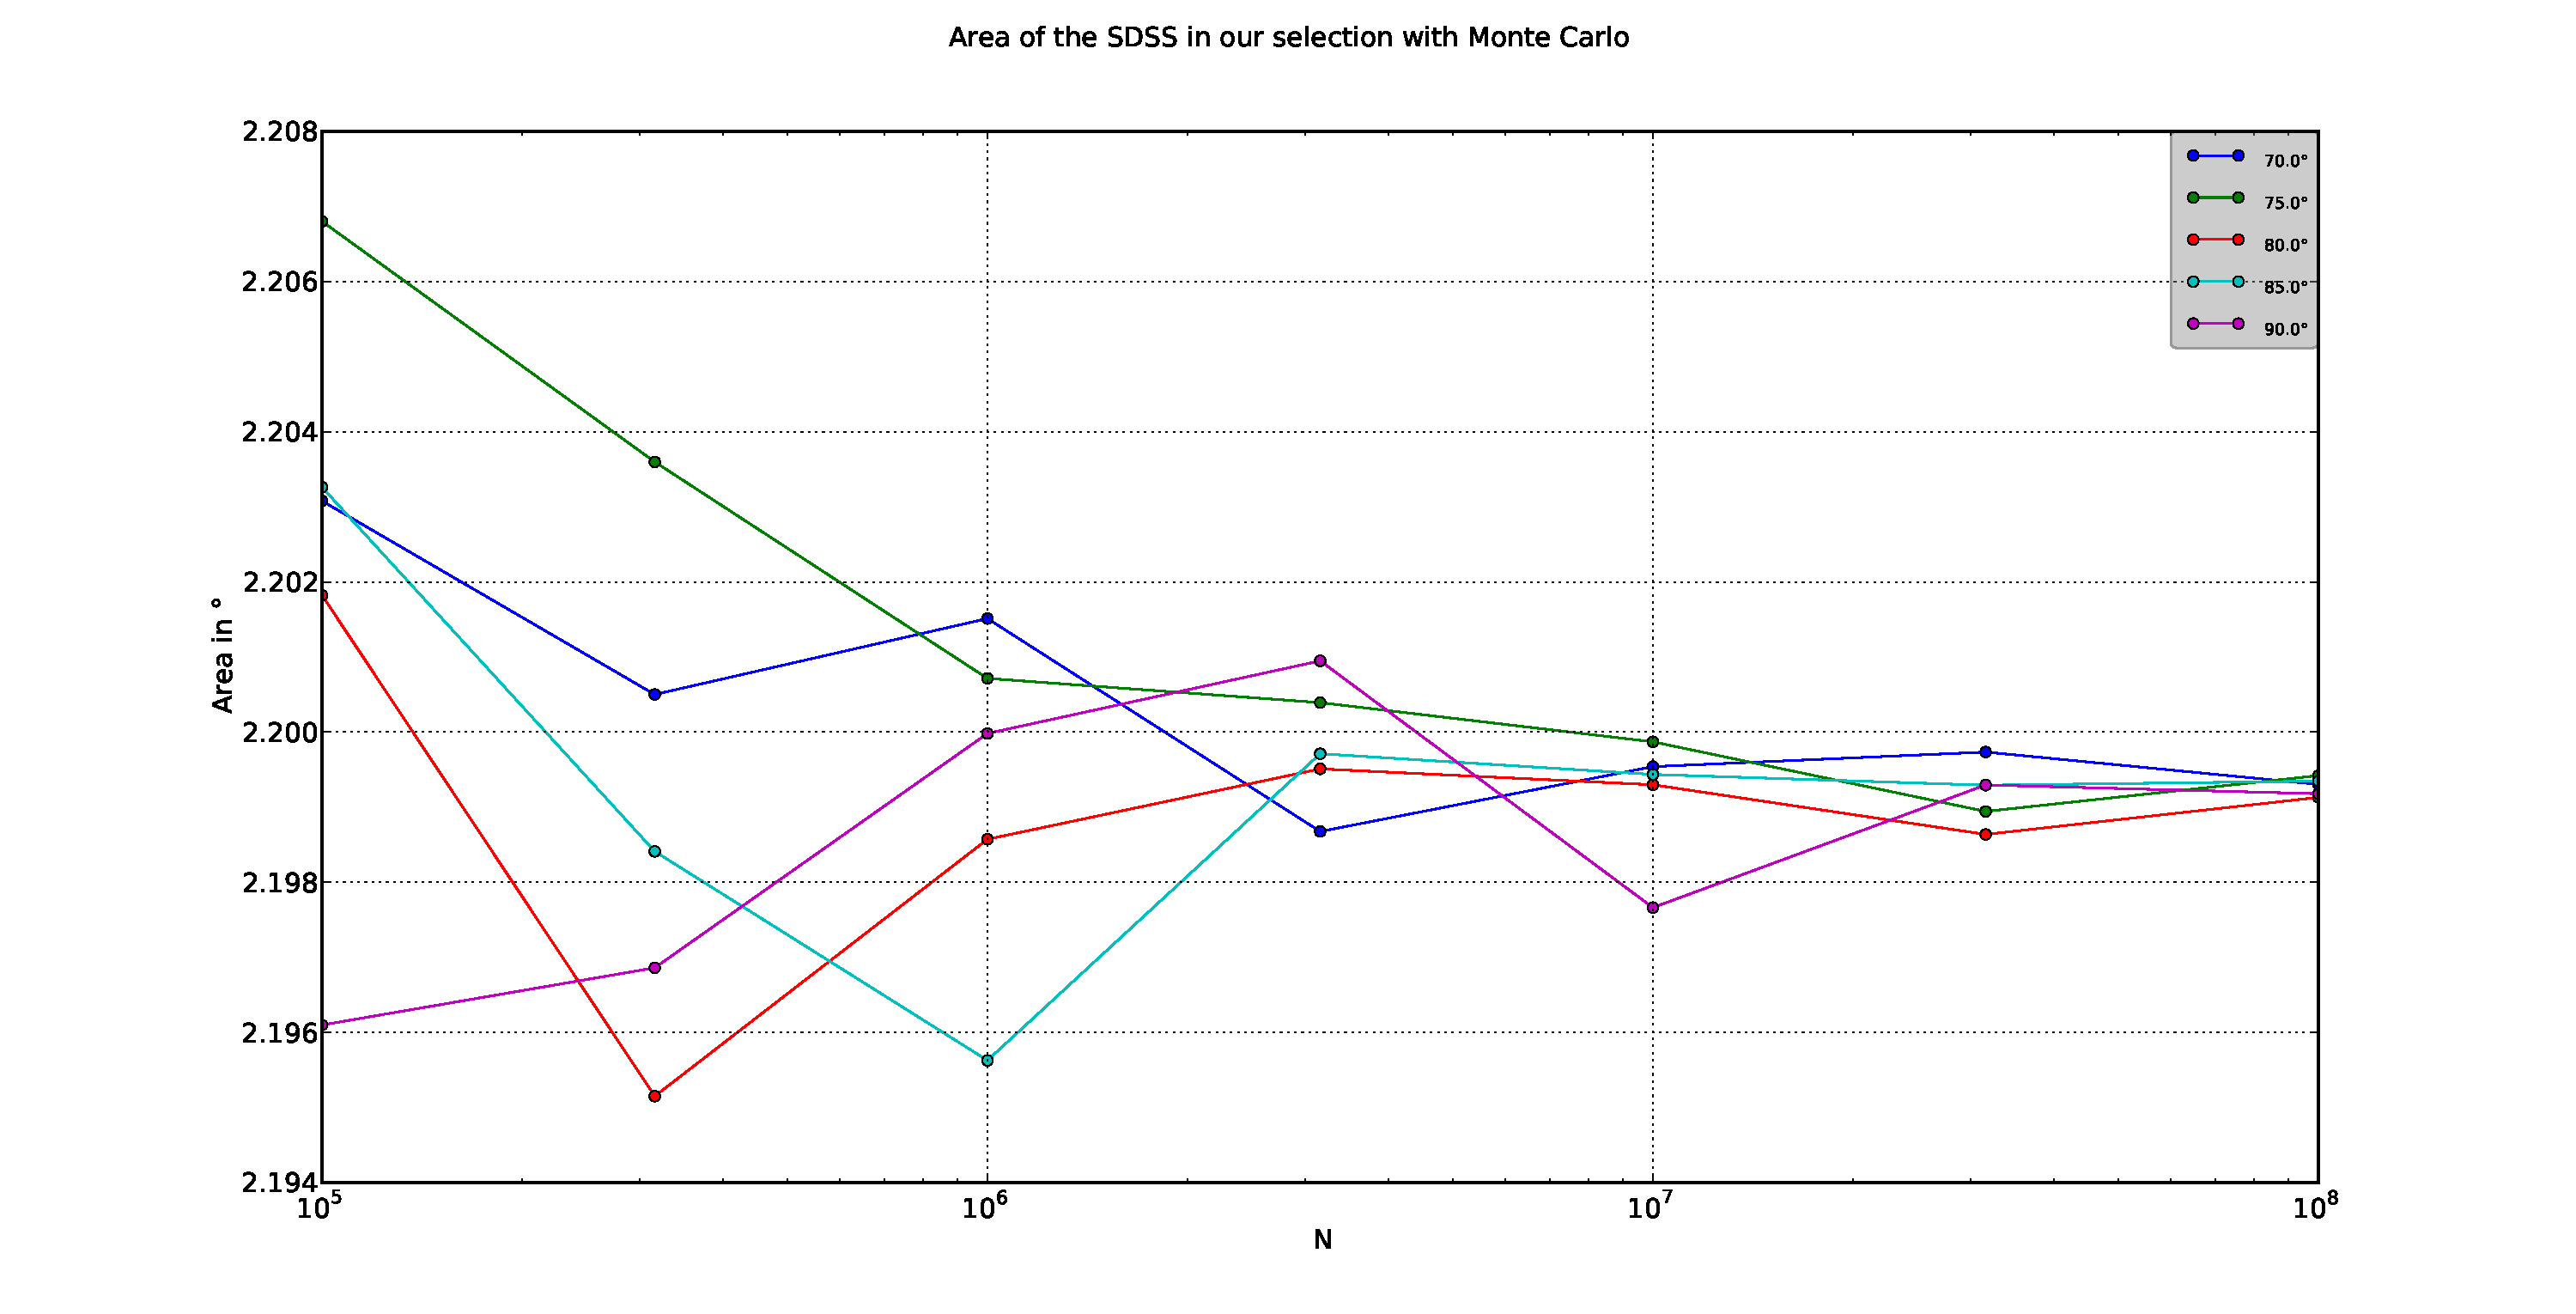
\includegraphics[height=0.4\textheight]{figures/sdss/SDSS_area}
        \captionof{figure}{Determination of the area of the SDSS for our
        selection with a Monte Carlo process. Results converge on a value of
    $2.1993\pm 0.0001$ steradians (i.e.\ roughly $7220\pm
\mathrm{\deg}^2$).\label{fig:sdss_area}}
    \end{minipage}
\end{figure}

\section{Coverage of the SDSS}

For many computations in this thesis, we need to determine the solid angle
covered by our galaxy sample. In the SDSS, the mask we constructed allows us to
do it easily by a Monte Carlo process.

First, we generate a number $N$ of points around a point of coordinates
$(\alpha_0, \delta_0)$ with a maximal angular separation $\theta_{\max}$ which
is larger than the maximal angular separation in our sample. The fraction of
points falling inside the mask gives us the fraction of the generated area
corresponding to the mask. This area is just
$\mathcal{S}=\int_0^{\theta_{\max}}\int_0^{2\pi}\sin\theta\dd{\theta}\dd{\phi}=
2\pi\left(1-\cos\theta_{\max}\right)$. We made this calculation for different
cone angles $\theta_{\max}$ and for different number of points to see if we
have a convergence in the value of the area. \bartreffigure{sdss_area} shows
that our geometry has a solid angle of $7220\pm1 \mathrm{\deg}^2$ but this
required five simulations with $10^8$ points.
%
\remark{%
    Generating points uniformly on the celestial sphere around a point of
    coordinates $(\alpha_0, \delta_0)$ to an angular distance $d$ can be done
    by assuming that this point is the upper pole of an other spherical system.
    In this situation, points follow $0\leqslant\theta\leqslant d$ and
    $0\leqslant\phi\leqslant2\pi$, assuming spherical coordinates and not
    celestial one. The azimuthal $\phi$ coordinates are generated as $2\pi U_1$
    where $U_1$ is a random variable following an uniform distribution between
    0 and 1. The latitude $\theta$ coordinates, follow
    $\left(p\left(\theta\right)=\cfrac{1}{2}\sin\theta\right)$ and are
    generated by $\theta=\arccos(2U_2-1)$, where $U_2$ is a variable following
    an uniform distribution with values between 0 and 1.

    Then, the points are rotated by quaternions to $(\alpha_0, \delta_0)$. The
    rotation axis is just the cross product between the pole vector and the
    vector defined by $(\alpha_0, \delta_0)$, and the rotation angle is
    $\cfrac{\pi}{2}-\delta_0$.
}

\section{Galaxy stellar masses}

In SDSS, contrary to coordinates, magnitudes or redshifts, stellar masses are
not measured by the SDSS pipelines. Instead, several teams have applied stellar
population models to the spectra and corrected their stellar masses from the
area subtended by the spectroscopic fiber to the entire galaxy, using the
apparent magnitudes within the fiber (fiberMag) and that extrapolated to the
entire galaxy (petroMag or modelMag). Indeed, contrary to coordinates,
magnitudes or redshifts, the stellar mass is not a direct observable. Its
estimation is based on the application of various stellar population models on
the galaxy spectrum observed by the SDSS\@. Several models exist, but they do
not provide the same estimation for a given galaxy. In
\bartreffigure{stellar_mass_models}, we compare eight models to have an order
of the inaccuracy of the stellar mass: FSPSGranWideDust, FSPSGranWideNoDust,
FSPSGranEarlyDust and FSPSGranEarlyNoDust from~\cite{Conroy+09}, PassivePort
and StarFormingPort from~\cite{Maraston+09}, PCAWiscM11 and PCAWiscBC03
from~\cite{Chen+12} and MPA-JHU from~\cite{Brinchmann+04, Kauffmann+03,
Tremonti+04}.

The principal discrepancies between the models come essentially from the
various stellar population synthesis (SPS) models involved in the fit of the
galaxy spectrum, necessary for the stellar mass estimation. But each model has
also some internal variations. For example,~\cite{Conroy+09} assume an early
star formation in galaxies for its FSPSGranEarlyNoDust (without dust extinction
correction) and FSPSGranEarlyDust (with dust extinction correction), while
FSPSGranWideDust and FSPSGranWideNoDust assume an extended star formation
history. As we can see, differences are relatively important: models using
different SPS have large dispersion in their estimation, while when using the
same SPS, stellar masses are coherent. Some models are also biased between each
other, but bias can be corrected and not considered in our analysis. Generally,
models agree to better than 0.3 dex, i.e.\ errors on individual masses are of
$0.3 / \sqrt{2} = 0.2$ dex. In particular, the MPA-JHU masses agree with all
others to typically better than 0.2 dex in $\sigma$.

\begin{figure}[htp]
    \centering
    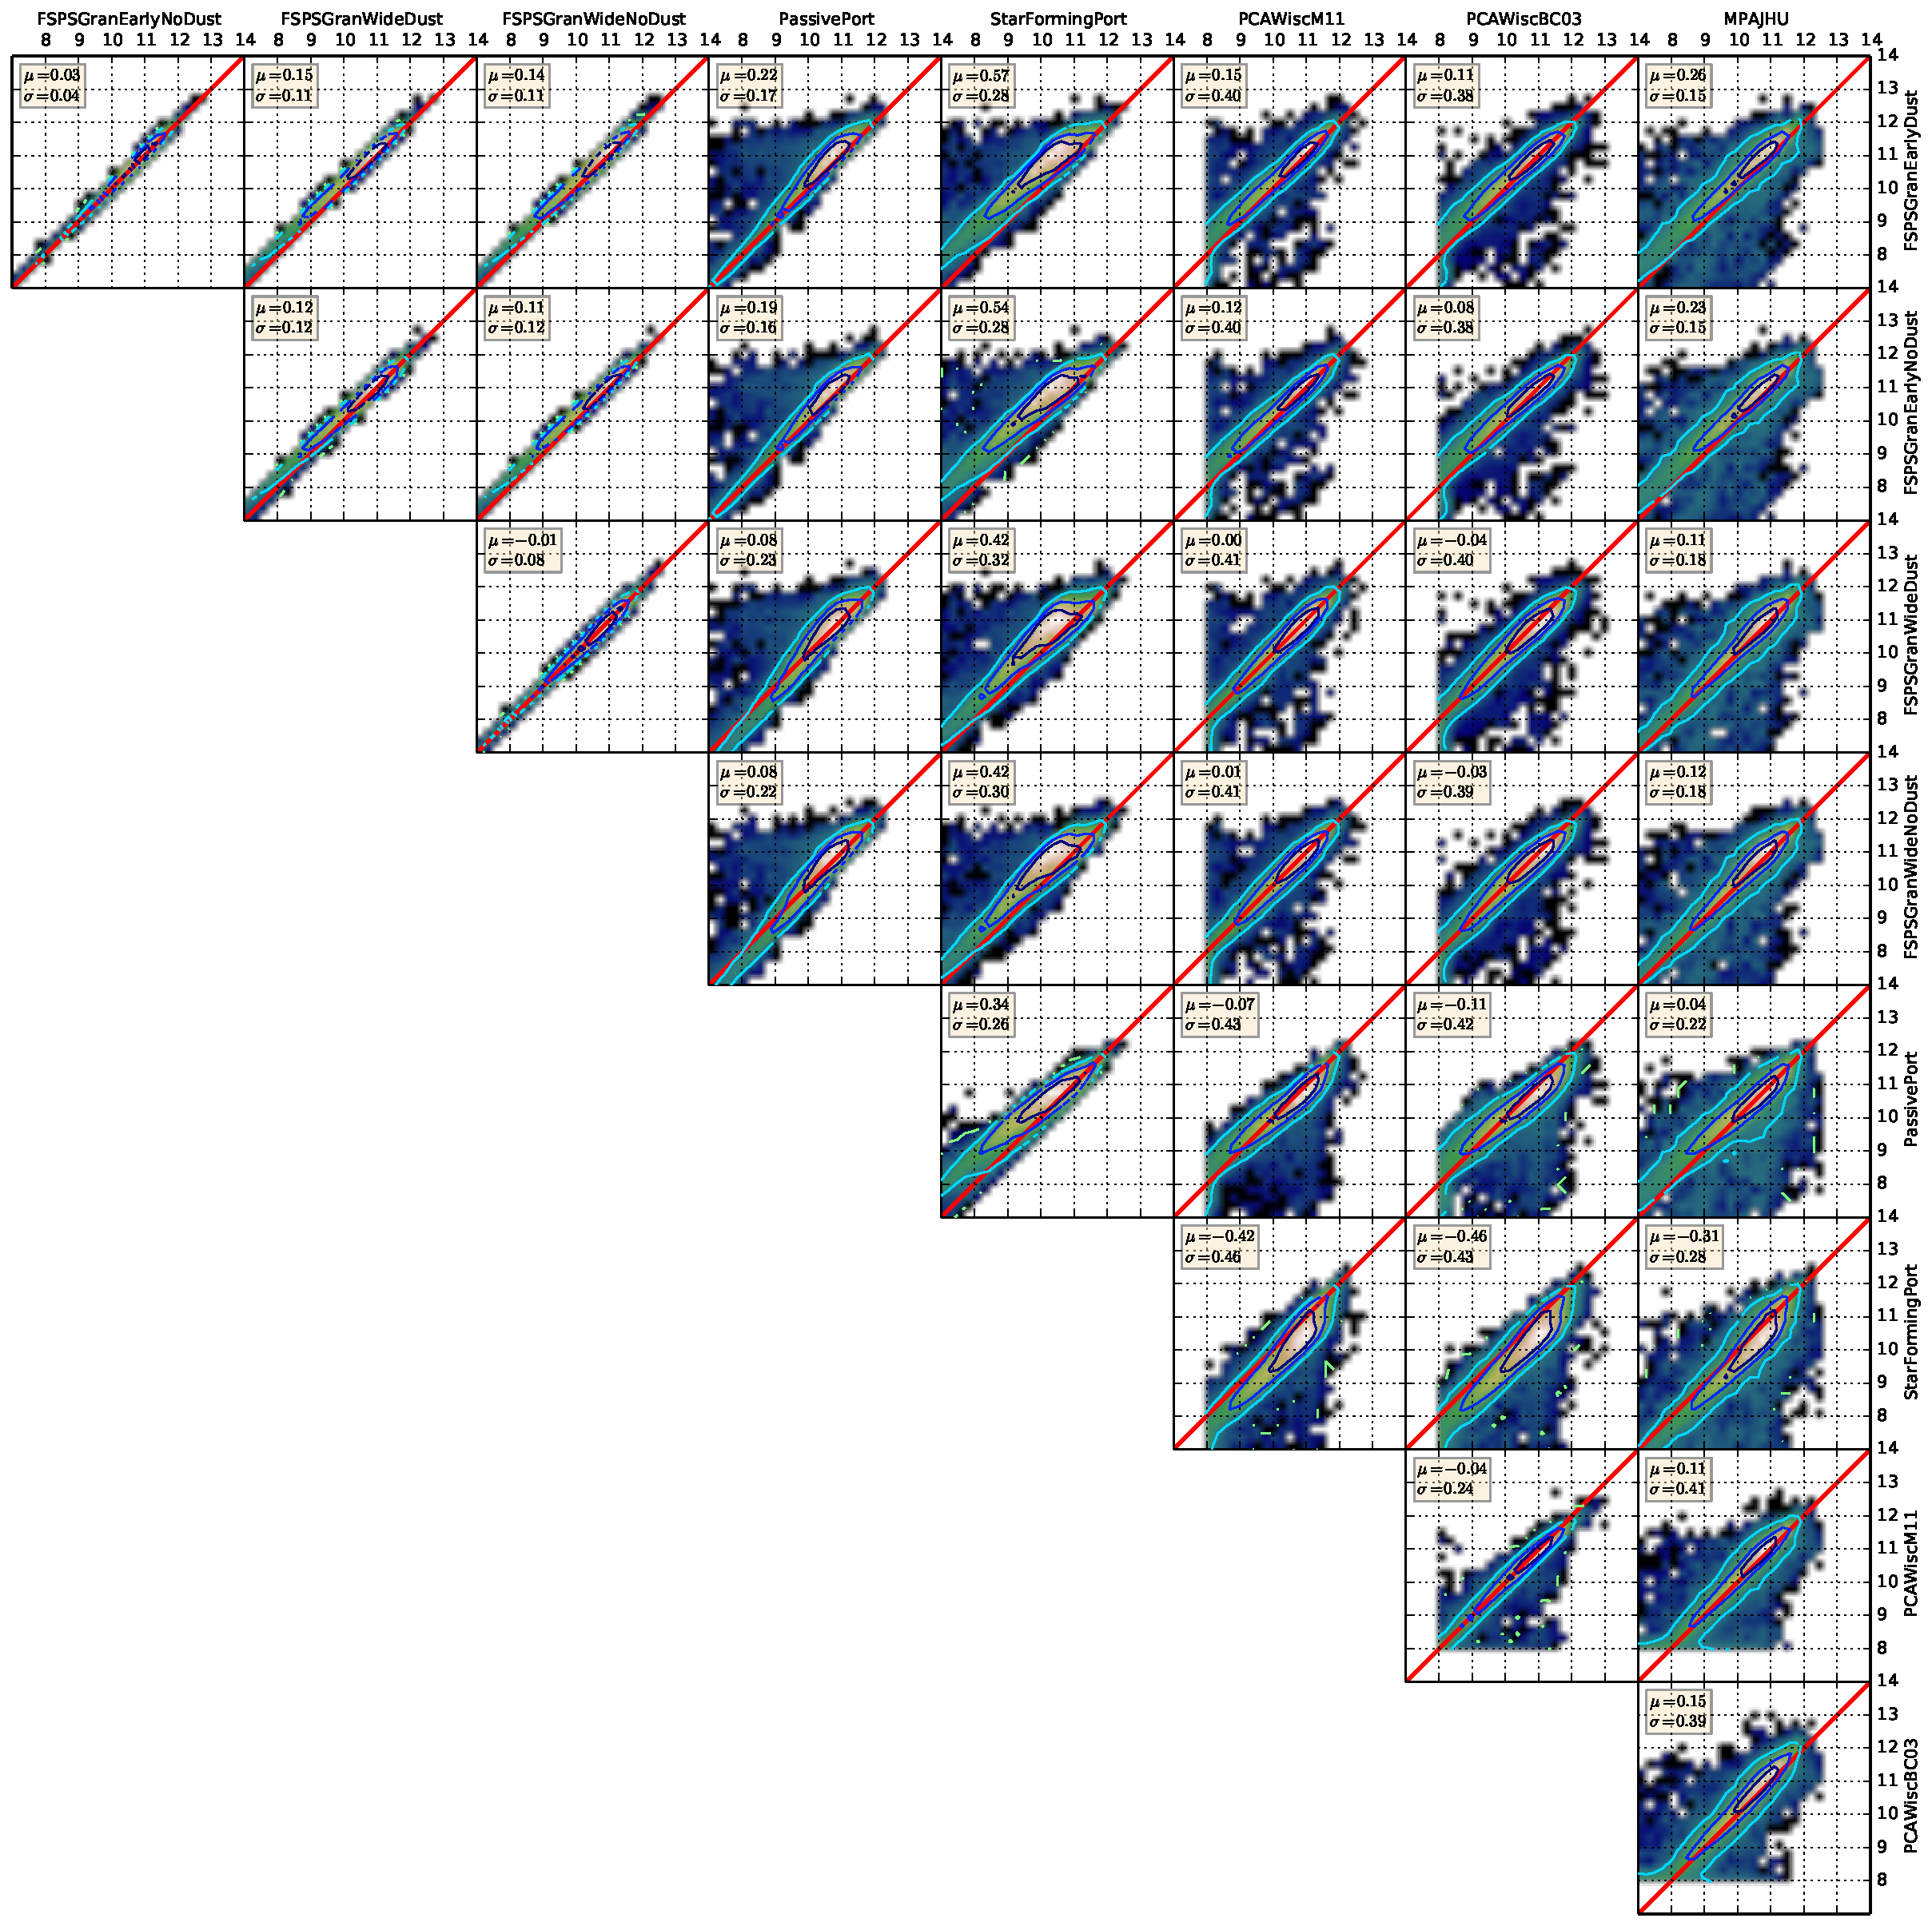
\includegraphics[width=\linewidth]{figures/sdss/stellar_mass_models.pdf}
    \caption{Comparison between stellar mass models applied onto galaxies from
        SDSS\@. Contours show the offsets in units of the scatter $\sigma$.
        Ordinates and abscissas are the logarithmic stellar masses of galaxies
        in the solar units. The upper left box shows the bias ($\mu$) and
        dispersion ($\sigma$) of the logarithmic difference between both
        models. The models are FSPSGranWideDust, FSPSGranWideNoDust,
        FSPSGranEarlyDust and FSPSGranEarlyNoDust \citep{Conroy+09},
        PassivePort and StarFormingPort \citep{Maraston+09}, PCAWiscM11 and
    PCAWiscBC03 \citep{Chen+12} and MPA-JHU~\citep{Brinchmann+04, Kauffmann+03,
Tremonti+04}.\label{fig:stellar_mass_models}}
\end{figure}

\section{Final galaxy sample}
\label{sec:final_galaxy_sample}

All previous sections are showing something important in the SDSS data:
observational errors can be important, and the automatic processing of this
data sometimes leads to false detections, artefacts\ldots, making analysis and
corrections complex.

Fortunately, recently in their FoF analysis of galaxy groups in the SDSS-DR10,
\cite{Tempel+14} had to deal too with such problems and the contamination they
introduce. Major problems are stars classified as galaxies, nearby large
galaxies fragmented into several galaxies or poor photometry of some galaxies
due to bright stars or bad sky level estimation in the neighbourhood. They
performed an impressive filtering on the sample by visually checking 30000
galaxies that were potentially problematic galaxies.~\cite{Tempel+14} thus
checked the following:
%
\begin{itemize}
    \item $10000$ apparently brightest galaxies (in $r$ band). For galaxies
        brighter than $m_r < 13.5$, about 10\% of the objects were spurious.
        For galaxies $13.5 < M_r < 14.5$, about 1\% were spurious entries; this
        fraction decreases with luminosity;
    \item $5000$ intrinsically brightest galaxies in the sample (< 1\% were
        spurious);
    \item $3000$ intrinsically faintest galaxies in the sample (to ensure the
        correctness of the faint-end of the luminosity function);
    \item all the sources with the spectroscopic class QSO\@;
    \item all the objects with \texttt{bestobjid} missing or not GALAXY\@. For
        these objects, they used \texttt{fluxobjid} if the matched photometric
        object was classified as a galaxy;
    \item all the objects for which the difference between $r$ band point
        spread function (PSF) magnitude and model magnitude was smaller than
        0.25 (thus further excluding some of the stellar sources in the
        catalogue);
    \item all the galaxies with the difference between $r$ band Petrosian and
        model magnitudes greater than 0.4;
    \item all the galaxy pairs that were closer than $5'$ (in order to remove
        double/multiple entries);
    \item the entries where the colour indices $g−r$, $r−i$, and $g−i$ had
        extreme values.
\end{itemize}

Finally,~\cite{Tempel+14} removed around $600$ galaxies, while $1400$ other
galaxies were flagged as having a bad photometry. We decided to use their
galaxy sample, since it covers exactly the same area we use and their
conscientious clean up of the SDSS-DR10 is difficult to surpass.

\subsection{Stellar masses}
\label{sub:stellar_masses}

Stellar masses are a major component of our algorithm, but~\cite{Tempel+14} did
not work with them, letting us the choice of the stellar masses to use. In
\bartreffigure{stellar_mass_models}, we show that there are large differences
between available models in the SDSS database. Estimations of some models are
different from the other and should not be used. A way to deal with this
problem is, for each galaxy in the sample, to use the median of the stellar
mass for all models. But sometimes, we don't have access to the stellar mass of
a galaxy and removing it from the sample will create supplementary
incompleteness. In such situations, we provide by default the
photometrically-based stellar mass estimation  of~\cite{Bell+03}. Those fitting
formulas allow to get the stellar mass of a galaxy directly from its color and
luminosity. Several colors are available to make the computation. We show in
\bartreffigure{bell_comparison} the stellar mass distribution for several
colors used on the formula of~\cite{Bell+03}. The $r-z$ color creates fewer
outliers in stellar masses than other bands. A possible explanation is that the
magnitude bands involved in the computation are less sensitive to dust
extinction and thus provide a more accurate estimation of stellar mass. So, we
adopt the stellar mass from $r-z$ color for those galaxies without spectral
mass estimates in the SDSS database.

\begin{figure}[htb]
    \centering
    \begin{minipage}{0.49\linewidth}
        \centering
        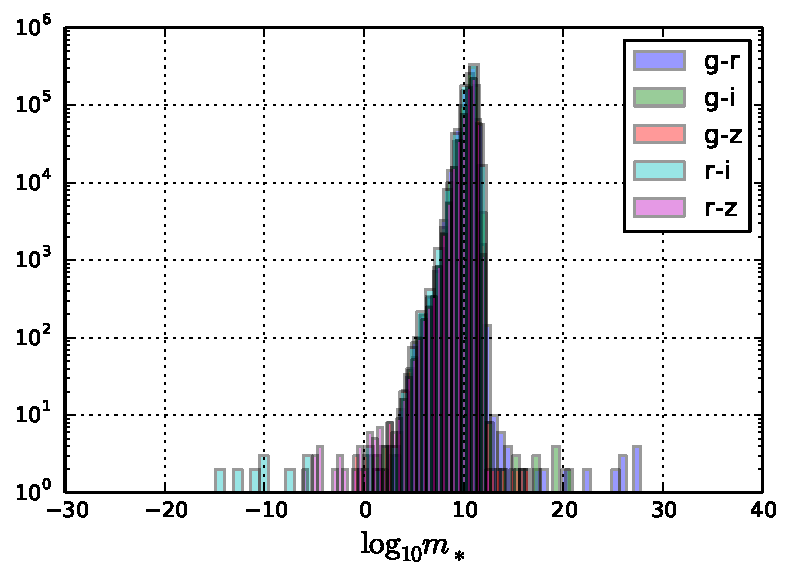
\includegraphics[width=\linewidth]{%
            figures/maggie_vs_sdss/bell_stellar_masses.pdf%
        }
        \captionof{figure}{The distribution of stellar masses for galaxies on
            the SDSS with the median of models described in
            \bartreffigure{stellar_mass_models} and the default value for
            galaxies without stellar mass estimations from~\cite{Bell+03} for
            different magnitude colors. The number of non-physical values for
            stellar masses is reduced by using the $r-z$ color, less affected
            by dust extinction and hence more
        accurate.\label{fig:bell_comparison}}
    \end{minipage}
    \begin{minipage}{0.49\linewidth}
        \centering
        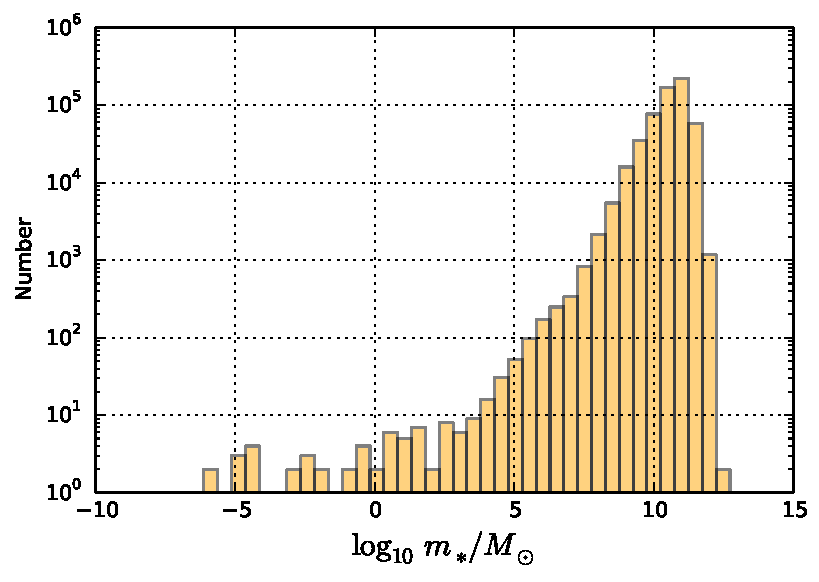
\includegraphics[width=\linewidth]{%
            figures/maggie_vs_sdss/sdss_stellar_masses_final.pdf%
        }
        \captionof{figure}{The distribution of stellar masses in solar units
            for our SDSS galaxy sample once chosen the $r-z$ color magnitude as
            default estimation. There are no high mass galaxies, but some
            stellar masses have unphysically low stellar masses. We keep them
            to avoid introducing supplementary incompleteness in the galaxy
        sample.\label{fig:stellar_mass_distribution}}
    \end{minipage}
\end{figure}

The resulting stellar mass distribution from our galaxy sample is shown in
\bartreffigure{stellar_mass_distribution}. No galaxies have too high stellar
masses, but a lot of them are very low and seems to not be physical. But we
can't remove them without introducing an incompleteness hence we keep them in
the sample.

\begin{figure}[htp]
    \centering
    \includegraphics[width=\linewidth]{%
        figures/maggie_vs_sdss/ssfr_models.pdf%
    }
    \caption{Comparison of several specific star formation rate (SSFR) measures
        from different models. FSPSGranWideDust, FSPSGranWideNoDust,
        FSPSGranEarlyDust and FSPSGranEarlyNoDust from~\cite{Conroy+09} and
        MPA-JHU~\cite{Brinchmann+04, Kauffmann+03, Tremonti+04}. Two variants
        exist for MPA-JHU according to if the estimation is based on the region
        of the fiber (suffixed \emph{fib}) or is also extrapolated (suffixed
        \emph{tot}). Axes are $\log_{10} \mathrm{SSFR}$ in units of
        $\mathrm{Gyr}^{-1}$. We show also the bias and dispersion of the
        log-difference of models. FSPS models are not very consistent between
        one another and we do not use them. MPA-JHU are relatively coherent but
    we should prefer the \emph{total} estimation since with the fiber
estimation not all the stellar population of the galaxy is
probed.\label{fig:sfr_comparison}}
\end{figure}

\subsection{Star formation rate}
\label{sub:star_formation_rate}

Measures of the star formation rate suffer the same problems as stellar masses:
the different models (from the same teams) do not necessarily agree with one
another. The comparison of the SFR measures (shown as the specific star
formation rate, SSFR = SFR divided by stellar mass) is shown on
\bartreffigure{sfr_comparison}. Some models disappeared: PCAWiscM11 and
PCAWiscBC03 do not provide SFR estimates for galaxies, while PassivePort and
StarFormingPort produce null SFR values for too many galaxies. MPA-JHU has
several estimates of the SFR\@: one based only on informations acquired by
the fiber pointing to the galaxy to get its spectrum (suffixed by \emph{fib})
and the other where an extrapolation of the informations is done outside the
aperture (suffixed by \emph{tot}).

\bartreffigure{sfr_comparison} shows that the SSFR values from the different
FSPS models are not consistent with one another, hence we did not use them in
our analysis. The bias and scatter between both models of MPA-JHU are small,
making them good measure of the SSFR of galaxies. Our preference goes to the
\emph{total} model, since the extrapolation used by the authors (at roughly
constant SSFR) must be better than none.

\begin{figure}[htb]
    \centering
    \includegraphics[width=0.8\linewidth]{%
        figures/maggie_vs_sdss/sfr_distribution.pdf%
    }
    \caption{The distribution of SSFR from the MPA-JHU model. We can see a
    bi-modality in the distribution, splitting galaxies into star forming
and passive galaxies (the \emph{green dashed} line shows the
separation).\label{fig:ssfr_distribution}}
\end{figure}

The resulting distribution of the SSFR in \bartreffigure{ssfr_distribution}
shows that galaxies can be classified into two categories: a star forming
population where an important fraction of the galaxy stellar mass is produced
in a time scale of $1$ Gyr and a passive one, where ongoing or recent star
formation represents a small fraction of its stellar mass. The green line in
\bartreffigure{ssfr_distribution} shows this limit. It will be useful when
searching if there is a modulation with the environment of the fraction of
young galaxies.

% vim: set tw=79 :

\bartchapterimage{heic0911b.jpg}
\chapter[MAGGIE vs SDSS]{MAGGIE versus SDSS}
\label{cha:MAGGIE_vs_SDSS}
\bartthumb{heic0911b.png}

\minitoc%

\section{Introduction}
\label{sec:vs_introduction}

MAGGIE is designed for an optimal extraction of galaxy groups in several
galaxy surveys such as the SDSS\@. Once the group catalogue in our
possession, we are able to analyze galaxies in both local and global
environments. Our study of environment is motivated by~\cite{Peng+10}
results, showing that with their estimation of the environment of galaxies,
the star formation rate (SFR) is independent of it, except for high mass
galaxies where the SFR is lower in dense environment. But as discussed in
the introduction of the thesis, the tracer used for the environment doesn't
distinguish between both environments. With our results, we make the same
analysis to see modulations with the projected radius in virial units and
the host halo mass.

\section{Environment modulation}
\label{sec:environment_modulation}

\cite{Peng+10} has shown that the mean SSFR is not very dependent of the
environment, using the over-density as a tracer. But we can go further and
see its modulation with local and global environment through the projected
radius of the galaxy in its halo and the virial mass of the host halo.

We tried this with both MAGGIE and the group catalogues provided
by~\cite{Tempel+14} for a simple comparison.

\subsection{MAGGIE}
\label{sub:ssfr_maggie}


\bartchapterimage{potw1252a.jpg}
\chapter{Conclusions and perspectives}
\label{cha:conclusions_and_perspectives}
\bartthumb{potw1252a.png}

\section{Conclusions}
\label{sec:conclusions}

The optimal extraction of galaxy groups from redshift space is not an easy
task. The observer has to deal with observational errors, projection
effects and bias to perform such an optimal grouping. We have argued that all
previously created galaxy group algorithms are imperfect in the sense that with
their assumptions, there are some lacks in extracted groups, explaining the
apparition of two different kind of algorithms: Bayesian and geometrical.

We constructed a galaxy mock catalogue to test several grouping algorithms. We
tested Friends-of-Friends algorithm to understand what is the optimal set of
linking lengths. We conclude that the choice of optimal linking lengths depends
on the science one wishes to do.

We created  MAGGIE, a Bayesian galaxy group finder, using probabilities to
constrain the membership in groups. The virial radii are estimated from either
the stellar mass (MAGGIE-m) or the luminosity (MAGGIE-L) of the central galaxy.
We show by tests on our mock catalogues that both implementations of MAGGIE
perform better on perfect data with no observational errors than the optimal
FoF algorithm. We also show that Bayesian algorithms as MAGGIE are more
sensitive to the quality of observational data than geometrical ones as FoF.
Nevertheless, both MAGGIE-m (with 0.02 dex errors in stellar masses) and
MAGGIE-L (with 0.08 dex errors in observed luminosities) perform better than
the optimal FoF, except at very high group masses, where the abundance matching
technique used in MAGGIE becomes inaccurate.

The application of MAGGIE on real galaxy surveys implies a full understanding
of the possible incompletenesses of these surveys. The analysis of the
SDSS-DR10 indicates that correcting for luminous and spectroscopic
incompletenesses is very important but also very difficult, since the
extraction of galaxy groups implies no missing galaxies. Incomplete membership
can affect the grouping, but also the informations obtained from their
analysis. Indeed, environmental effects we wish to observe in galaxy groups
(essentially through the SSFR) can be very sensitive to the way incompleteness
is handled. Therefore, MAGGIE is a very powerful tool for galaxy group analysis, but we have
to apply it carefully on the analysed data or the interpretation of results can
be biased.

\section{Perspectives}
\label{sec:perspectives}

We plan to run MAGGIE on the SDSS-DR10 and publish optimized galaxy groups in
different doubly complete subsamples in redshift and luminosity, and to
re-assess the modulation of sSFR, etc\ldots with local and global environments.
If a modulation of galaxy properties is observed, we will model it and apply it
in semi-analytical codes to see if it reduces discrepancies between
observations and outputs of such codes. It will be a new measure of quenching
of star formation with global and local environments. We also wish to run
MAGGIE on the deeper GAMA redshift survey to be able to extract the evolution
in time of environmental effects on galaxies. We already have some preliminary
results on this modulation applying MAGGIE on the SDSS\@.
\bartreffigure{ssfr_mean} and \bartreffigure{ssfr_fraction} show the median
SSFR and the fraction of non-passive galaxies with local and global environment
for the SDSS, and the same for group catalogues of~\cite{Tempel+14} in
\bartreffigure{ssfr_mean_tempel} and \bartreffigure{ssfr_fraction_tempel}. We
use two complete catalogues to show this modulation: catalogue 3 too have
sufficient statistics in number of galaxies and catalogue 5 to see the
behaviour at larger redshifts.

\begin{figure}[htb]
    \centering
    \begin{minipage}{\linewidth}
        \centering
        \begin{minipage}{\linewidth}
            \centering
            \subfloat[Catalogue 3]{%
                \includegraphics[height=0.2\textheight]{%
                    {figures/maggie_vs_sdss/sdss.0.mean_ssfr_2}.pdf%
                }
            }
        \end{minipage}
        \begin{minipage}{\linewidth}
            \centering
            \subfloat[Catalogue 5]{%
                \includegraphics[height=0.2\textheight]{%
                    {figures/maggie_vs_sdss/sdss.0.mean_ssfr_4}.pdf%
                }
            }
        \end{minipage}
        \captionof{figure}{Mean SSFR for galaxies with
            $10\leqslant\log_{10}m_*<11$ (left panel) and
            $11\leqslant\log_{10}m_*<12$ as a function of the projected radius
            in units of virial radius (local environment) and of the virial
            mass in solar units (global environment), for galaxy groups
        found with MAGGIE.\label{fig:ssfr_mean}}
    \end{minipage}
    \begin{minipage}{\linewidth}
        \centering
        \begin{minipage}{\linewidth}
            \centering
            \subfloat[Catalogue 3]{%
                \includegraphics[height=0.2\textheight]{%
                    {figures/maggie_vs_sdss/sdss.0.fraction_over_minus_2_2}.pdf%
                }
            }
        \end{minipage}
        \begin{minipage}{\linewidth}
            \centering
            \subfloat[Catalogue 5]{%
                \includegraphics[height=0.2\textheight]{%
                    {figures/maggie_vs_sdss/sdss.0.fraction_over_minus_2_4}.pdf%
                }
            }
        \end{minipage}
        \captionof{figure}{Fraction of galaxies classified as star forming
            galaxies according the criterion of
            \bartrefsubsection{star_formation_rate} for the same range in
            stellar masses as in \bartreffigure{ssfr_mean}, with galaxy group
            from MAGGIE.\label{fig:ssfr_fraction}}
    \end{minipage}
\end{figure}

\begin{figure}[htb]
    \centering
    \begin{minipage}{\linewidth}
        \centering
        \begin{minipage}{\linewidth}
            \centering
            \subfloat[Catalogue 3]{%
                \includegraphics[height=0.2\textheight]{%
                    {figures/maggie_vs_sdss/tempel.0.mean_ssfr_2}.pdf%
                }
            }
        \end{minipage}
        \begin{minipage}{\linewidth}
            \centering
            \subfloat[Catalogue 5]{%
                \includegraphics[height=0.2\textheight]{%
                    {figures/maggie_vs_sdss/tempel.0.mean_ssfr_4}.pdf%
                }
            }
        \end{minipage}
        \captionof{figure}{Same as \bartreffigure{ssfr_mean} but for galaxy
        groups from~\cite{Tempel+14}.\label{fig:ssfr_mean_tempel}}
    \end{minipage}
    \begin{minipage}{\linewidth}
        \centering
        \begin{minipage}{\linewidth}
            \centering
            \subfloat[Catalogue 3]{%
                \includegraphics[height=0.2\textheight]{%
                    {figures/maggie_vs_sdss/tempel.0.fraction_over_minus_2_2}.pdf%
                }
            }
        \end{minipage}
        \begin{minipage}{\linewidth}
            \centering
            \subfloat[Catalogue 5]{%
                \includegraphics[height=0.2\textheight]{%
                    {figures/maggie_vs_sdss/tempel.0.fraction_over_minus_2_4}.pdf%
                }
            }
        \end{minipage}
        \captionof{figure}{Same as \bartreffigure{ssfr_fraction} but for
        galaxy groups
    from~\cite{Tempel+14}.\label{fig:ssfr_fraction_tempel}}
    \end{minipage}
\end{figure}
%
The modulation of the SSFR and fraction of young galaxies is very dependent of
the catalogue of groups used. Since these results between the two algorithms, a
deeper analysis must be done to understand from where the discrepancies come
from.

Still for MAGGIE, we plan to improve the galaxy grouping by the use of the
red-blue segregation of galaxies. We can use some priors for the modulation of
the fraction of blue galaxies in groups to adapt the probability computation
according to the class of the galaxy. Then, we can iteratively reduce the
impact of our initial model for the blue fraction by using the informations
obtained by MAGGIE to de-project the red-blue segregation observed in groups.
For next iterations, we can re-use our new real space model in the probability
computation, and do it until the convergence of memberships.

In parallel, we plan to launch a collaborative project with other grouping
algorithm developers. We will propose to each developer (and myself) to apply
their algorithms to a set of mock catalogs constructed in the same way to avoid
cosmic variance on the results, for blind tests. Then, we will run the same
tests on each algorithm in order to have a clear understanding of the strengths
and weaknesses of each of them. It will be the first time that galaxy grouping
algorithms will be compared in the same conditions.

Given that imperfect grouping algorithms wash out the observable environmental
effects, it is also interesting to know if there is a limit to recover the real
space modulation of galaxy properties (such as specific star formation rate)
with environment when trying to extract it from projected redshift space. This
can be easily done by imposing ourselves a modulation in the outputs of galaxy
formation codes, and then construct galaxy mock catalogues in redshift space.
We can then see if the imposed modulation is recovered in the observations, and
if galaxy group algorithms introduce biases in some cases. This will allow one
to determine the maximum level of environmental dependence of star formation
quenching that is consistent with the observations.

In continuation with the thesis work, we can try to theoretically explain the
observed dependency of galaxy properties with their environments. Using
hydrodynamical simulations of galaxies in groups, we wish to understand and
model intra-cluster physical processes (ram pressure stripping, tidal
stripping\ldots). This will imply running academic simulations independently
for each physical process, then model as a function of the different input
parameters (local and global environment essentially). And by trying to switch
them on-off in semi-analytical codes of galaxy formation, determine their
relative importance on galaxy properties (sSFR, bulge to disk ratios\ldots).

% vim: set tw=79 :


%
\appendix

% adding files for the appendix
\bartchapterimage{heic0911c.jpg}
\chapter{Density profiles}
\label{cha:profiles}
\bartthumb{heic0911c.png}

\section{Introduction}

In this chapter, we provide details on the computation of the density profiles
and their derived quantities. We define here the different normalizations used
along the thesis for some popular density profiles.

\subsection{Definitions}

The number of galaxies in a sphere of radius $r$ with a density profile in
number $\nu(r)$ is the case of a spherical symmetry:
%
\begin{equation}
    N\left(r\right)=\int_0^r4\pi {r'}^2 \nu(r')\dd{r'}
\end{equation}

To start, we define some dimensionless functions to facilitate the
computations.
%
\begin{eqnarray}
    N\left(r\right)&=N\left(a\right){\widetilde{N}\left(r/a\right)}\nonumber\\
    \nu\left(r\right)&=
        \cfrac{N\left(a\right)}{4\pi{a^3}}
        \,\widetilde\nu\left(r/a\right)
\end{eqnarray}
%
with $a$ the radius at which the logarithmic slope of the density profile is
equal to $-2$. We also define the same relations for a
virial normalization.
%
\begin{eqnarray}
    N\left(r\right)&={N_v}\,{\widehat{N}\left(r/\rvir\right)}\nonumber\\
    \nu\left(r\right)&=
        \cfrac{N_v}{4\pi\rvir^3}\,\widehat\nu\left(r/\rvir\right)
\end{eqnarray}

We also define the concentration $c$ as the ratio between the virial radius
$\rvir$ and the radius $a$, i.e.\ $c=\rvir/a$. We define $\rvir=r_{200}$ for
simplicity.

\section{Density profiles}
\label{sec:density_profiles}

\subsection{\citet{NFW+97}}

The NFW density profile is:
%
\begin{equation}
    \nu \left(r\right) = \cfrac{\nu_0}{r {\left(r+a\right)}^2}
\end{equation}
%
with $\nu_0$ a constant density.

We can write by integrating previous relations with $\int_0^1
x^2\widetilde\nu\dd x=\int_0^1 x^2\widehat\nu\dd x$  and searching for the
constant $\nu_0$:
%
\begin{equation}
    \widetilde\nu\left(x\right)=\cfrac{1}{\ln2-1/2}
        \quad\cfrac{1}{x{\left(1+x\right)}^2}
\end{equation}
%
\begin{equation}
    \widetilde{N}\left(x\right)=\cfrac{1}{\ln2-1/2}
        \quad\left(\ln\left(1+x\right)-\cfrac{x}{x+1}\right)
\end{equation}
%
\begin{equation}
    \widehat\nu\left(x\right)=
        \cfrac{1}{\ln\left(1+c\right)-c/ \left(1+c\right)}
        \quad\cfrac{1}{x{\left(1/c+x\right)}^2}
\end{equation}
%
\begin{equation}
    \widehat{N}\left(x\right)=
        \cfrac{1}{\ln \left(1+c\right)-c/ \left(1+c\right)}
        \quad\left(\ln\left(1+xc\right)-\cfrac{xc}{xc+1}\right)
\end{equation}

\subsection{Einasto}
\label{sub:einasto}

For an Einasto density profile:
\begin{equation}
    \nu \left(r\right) = \nu_0 \exp
    \left[- {\left(\cfrac{r}{b}\right)}^{1/m}\right]
\end{equation}

Writing the definition of the $a$ radius with this density profile, we have:
%
\begin{equation}
    {\left(\cfrac{1}{b}\right)}^{1/m} = 2m{\left(\cfrac{1}{a}\right)}^{1/m}
\end{equation}
%
leading to the following normalizations:
%
\begin{equation}
    \widetilde\nu \left(x\right) = \cfrac{{\left(2m\right)}^{3m}}{m\gamma
    \left(3m, 2m\right)} \exp \left(-2mx^{1/m}\right)
\end{equation}
%
\begin{equation}
    \widetilde{N} \left(x\right) = \cfrac{\gamma \left(3m, 2m
    x^{1/m}\right)}{\gamma \left(3m, 2m\right)}
\end{equation}
%
\begin{equation}
    \widehat\nu \left(x\right) = \cfrac{{\left(2m\right)}^{3m}}{m\gamma
    \left(3m, 2m c^{1/m}\right)} \exp \left(-2m{\left(xc\right)}^{1/m}\right)
\end{equation}
%
\begin{equation}
    \widehat{N} \left(x\right) = \cfrac{\gamma \left(3m, 2m
        {\left(xc\right)}^{1/m}\right)}{\gamma \left(3m, 2m c^{1/m}\right)}
\end{equation}

\subsection{Generalized NFW}
\label{sub:generalized_nfw}

If any previous density profiles isn't sufficient to describe the distribution
of dark matter particles or galaxies inside the halos, a solution is possibly
to fit a generalized NFW profile, whose the density is:
%
\begin{equation}
    \nu \left(r\right) =
    \cfrac{\nu_0}{r^\alpha{\left(r+a\right)}^{\beta-\alpha}}
\end{equation}

In this case:
%
\begin{equation}
    \widetilde{N} \left(x\right) = \cfrac{%
        \mathcal{B}_{-x} \left(3-\alpha, 1+\alpha-\beta\right)}
    {\mathcal{B}_{-1} \left(3-\alpha, 1+\alpha-\beta\right)}
\end{equation}
%
therefore:
%
\begin{equation}
    \widetilde\nu \left(x\right) = \cfrac{1}
    {{\left(-1\right)}^{\alpha+1}
        \mathcal{B}_{-1} \left(3-\alpha, 1+\alpha-\beta\right)}
    \quad\cfrac{1}
    {x^\alpha {\left(1+x\right)}^{\beta-\alpha}}
\end{equation}
%
For the virial normalization:
%
\begin{equation}
    \widehat{N} \left(x\right) = \cfrac{%
        \mathcal{B}_{-xc} \left(3-\alpha, 1+\alpha-\beta\right)}
    {\mathcal{B}_{-c} \left(3-\alpha, 1+\alpha-\beta\right)}
\end{equation}
%
\begin{equation}
    \widehat\nu \left(x\right) = \cfrac{1}
    {{\left(-1\right)}^{\alpha+1}
        \mathcal{B}_{-c} \left(3-\alpha, 1+\alpha-\beta\right)}
    \quad\cfrac{1}
    {{\left(xc\right)}^\alpha {\left(1+xc\right)}^{\beta-\alpha}}
\end{equation}
%
where $\mathcal{B}$ is the function defined as:
%
\begin{equation}
    \mathcal{B} \left(a, b\right) =
    \cfrac{\Gamma \left(a\right) \Gamma \left(b\right)}
    {\Gamma \left(a+b\right)} =
    \int_0^1 t^{a-1} {\left(1+t\right)}^{b-1} \dd t
\end{equation}
%
and its incomplete version is:
%
\begin{equation}
    \mathcal{B}_z \left(a, b\right) =
    \int_0^z t^{a-1} {\left(1+t\right)}^{b-1} \dd t
\end{equation}

\section{Radial velocity dispersion}
\label{sec:radial_velocity_dispersion}

Galaxies in groups (and their associated dark matter halos) are assumed to be a
system of particles only submitted to the gravitation. Neglecting mergers and
other physical processes inside galaxy groups, the number of galaxies doesn't
evolve in phase space, and the distribution function is constant along the
evolution of the system. In this case, we can use the collisionless Boltzmann
equation to extract dynamical properties of galaxy groups.

The Jeans equation is the first velocity momentum of the Boltzmann equation. In a
spherical symmetry, assuming stationarity, the Jeans equation is:
%
\begin{equation}
    \label{eq:jeans}
    \ddp{\left[\nu(r)\sigma_r^2(r)\right]}{r} +
    \cfrac{2\mybeta}{r}\left[\nu(r)\sigma_r^2(r)\right]=
    -\nu(r)\cfrac{GM(r)}{r^2}
\end{equation}
%
where $\beta \left(r\right)$ is the radial profile of velocity anisotropy
$\beta = 1 - \sigma_\theta^2/\sigma_r^2$.

We can compute the radial velocity dispersion using \bartrefequation{jeans} for
a spherical system at equilibrium. The solution to this equation is given by:
%
\begin{equation}
    \myprofil\sigma_r^2(r)=
    \int_r^\infty K_r(r,s)\nu(s)\cfrac{GM(s)}{s^2}\,\dd{s}
\end{equation}
%
with $K_r(r,s)$ the kernel of the integral defined as:
%
\begin{equation}
    K_r(r,s)=\exp\left[2\int_r^s\mybeta\cfrac{\dd{t}}{t}\right]
\end{equation}

There are two ways of normalizing the radial velocity dispersion according to
the normalization used for the density and mass profiles. We show it for the
virial normalization for illustration:
%
\begin{equation}
    \label{eq:sigma_norm}
    \widehat\sigma_r^2(x)= \cfrac{1}{\widehat\nu \left(x\right)}
    \int_x^\infty K_r(x,s)\widehat\nu(s)\cfrac{\widehat{M}(s)}{s^2}\,\dd s
\end{equation}
%
with:
%
\begin{equation}
    \sigma_r^2(r) = \cfrac{GM_v}{\rvir}\,\widehat\sigma_r^2(r/\rvir)
\end{equation}

We are interested only in the NFW profile in the thesis, since it is accurate
enough to adjust the model. If we want an analytical form for $\sigma_r
\left(r\right)$, we need to choose a model for the anisotropy profile $\beta
\left(r\right)$. We provide here some expressions of the radial velocity
dispersion, assuming the NFW density profile, for a useful anisotropy model.

\subsection{\citet{ML+05}}
\label{sub:ml05}

This model is of the form:
%
\begin{equation}
    \beta \left(r\right) = \undemi\cfrac{r}{r+b}
\end{equation}
%
where $b$ is a characteristic radius of the model. Introducing this expression
in \bartrefequation{sigma_norm}, we obtain:
%
\begin{align}
    \widetilde\sigma_r^2(x)=&
        -\frac{1}{3 x (1+r x)
        {(-1+\ln\left(4\right))}^2}2
        \left(-\frac{1}{2}+\ln\left(2\right)\right)\nonumber\\
    &\left(x \left(3+x \left(\pi ^2 (-3+2 r)
        {(1+x)}^2-3 (-9+5 r-7 x+4 r x)
        \right)\right.\vphantom{\ln\left(1+\frac{1}{x}\right)}\right.
        \nonumber\\
    &\left.-3 x^3 \ln\left(1+\frac{1}{x}\right)+3 x (1+2 x)
        \ln\left(x\right)\right)\nonumber\\
    & -3 (1+2 x (-1-2 x (2+x)+r (1+x) (1+2 x)))
        \ln\left(1+x\right)+3 (-3+2 r) {\left(x+x^2\right)}^2
        \ln{\left(1+x\right)}^2\nonumber\\
    & \left.+6 (-3+2 r) x^2 {(1+x)}^2
        Li_2\left(-x\right)\vphantom{\ln\left(1+\frac{1}{x}\right)}\right)
        \nonumber\\
\end{align}
\begin{align}
    \widehat\sigma_r^2(x)=&
        \frac{1}{6 x (1+r x) \left(-1+\frac{1}{1+c}+\ln c\right)}
        \left(c x \left(-3+x \left(3 c \left(-9+\pi ^2\right)+
        \left(15-2 \pi ^2\right) r\right.\right.
        \vphantom{{(1+c x)}^2}\right.\\
    &\left. -4 c \left(-3+\pi ^2\right) r x+
        3 c^3 \pi ^2 x^2+c^2 x \left(-21+\pi ^2 (6-2 r x)\right)\right)\\
    & \left.+6 c^3 x^3 {\rm arccoth} \left(1+2 c x\right)-
        3 c x (1+2 c x) \ln\left(c x\right)\right)\\
    &+3(1+2 x (r+c (-1+x (-4 c+3 r+2 c (-c+r) x))))
        \ln\left(1+c x\right)\\
    &\left.+3c(3 c-2 r) x^2 {(1+c x)}^2 {\left(\ln\left(1+c x\right)\right)}^2+
    6 c (3 c-2 r) x^2 {(1+c x)}^2 \mathrm{Li_2}\left(-c x\right)\right)\\
\end{align}

\section{Line of sight velocity variance}

We will compute in this section the line of sight velocity dispersion of
galaxies in a general spherical density profile, and then compute it
specifically for an NFW profile. This is useful to make cuts at
$\pm\kappa\sigma_\mathrm{LOS} \left(R\right)$ in the \pps{}.

By definition, the variance is the mean of the squared quantity. We use a
general density profile which is invariant under rotations $\nu{(r)}$. In our
case, we make this mean on the line of sight, so:
%
\begin{equation}
    \sigma_\mathrm{LOS}^2\left({R}\right)=
    \cfrac{\int_{-\infty}^{\infty}{v_\mathrm{LOS}^2}\nu{(r)}\,\dd{z}}
    {\int_{-\infty}^{\infty}\nu{(r)}\,\dd{z}}
\end{equation}
%
But in the group, $r^2=R^2+z^2$ so:
%
\begin{equation}
    \sigma_\mathrm{LOS}^2\left({R}\right)=
    \cfrac{2\int_{R}^{r_{\max}}{v_\mathrm{LOS}^2}
    \cfrac{\nu{(r)}{r}}{\sqrt{r^2-R^2}}\,\dd{r}}
    {2\int_{R}^{r_{\max}}\cfrac{\nu{(r)}{r}}{\sqrt{r^2-R^2}}\,\dd{r}}
\end{equation}
%
The denominator is by definition the projected density surface along the line
of sight and we denote it
%
\begin{equation}
    \Sigma(R) = 2\int_{R}^{r_{\max}}\cfrac{\nu{(r)}{r}}{\sqrt{r^2-R^2}}\,\dd{r}
\end{equation}
%
Normally the integration is for $r_{\max}\rightarrow\infty$ but in our case we
want to restrict to a limited region in the group (to the virial sphere
precisely).

In the same coordinate system as previously, the line of sight velocity can be
expressed in spherical coordinates as:
%
\begin{equation}
    v_{\mathrm{LOS}} = v_r \cos\theta - v_\theta \sin\theta
\end{equation}
%
We suppose that we are at the equilibrium and so that there is no flow in the
group in consequence we can neglect means of velocities. In terms of velocity
variance we have now:
%
\begin{equation}
    \mysigma\mysiglos = 2\int_R^{r_{\max}}
    \left({\sigma_r^2(r)\cos^2\theta+\sigma_\theta^2\sin^2\theta}\right)
    \cfrac{\nu{(r)}{r}}{\sqrt{r^2-R^2}}\,\dd{r}
\end{equation}
%
If we want to use the anisotropy parameter
$\mybeta=1-\sigma_\theta^2(r)/\sigma_r^2(r)$ in case of sphericity, we can
write:
%
\begin{equation}
    \mysigma\mysiglos = 2\int_R^{r_{\max}}
    \left({1-\mybeta\cfrac{R^2}{r^2}}\right)
    \cfrac{\nu{(r)}{\sigma_r^2(r)}{r}}{\sqrt{r^2-R^2}}\,\dd{r}
\end{equation}

We can compute the radial velocity dispersion using the Jeans equation for a
spherical system at equilibrium.

\subsection{\citet{ML+05} anisotropy}

With the decomposition of the integral over the domain of integration, we can
write:
%
\begin{align}
    \Sigma{(R)}{\sigma_\mathrm{LOS}}^2{(R)}=&
        2\int_R^{r_v}{\cfrac{\left({s+a}\right)}{s^2}{\nu(s)}{G}{M(s)}}{\dd{s}}
        \nonumber\\
    &\times
        \left(\int_R^s{\left(\cfrac{r}{r+a}-\undemi
        {\left(\cfrac{R}{r+a}\right)}^2\right)
        \cfrac{1}{\sqrt{r^2-R^2}}\dd{r}}\right)\nonumber\\
    &+2\int_{r_v}^{\infty}
        \cfrac{\left({s+a}\right)}{s^2}\nu(s){G}{M(s)}\dd{s}\nonumber\\
    &\times
        \left(\int_R^{r_v}
            \left(\cfrac{r}{r+a}-\undemi{\left(\cfrac{R}{r+a}\right)}^2\right)
            \cfrac{1}{\sqrt{r^2-R^2}}\dd{r}\right)
\end{align}
%
where we are setting $r_{\max}$ to $r_v$. So now we can write:
%
\begin{align}
    {\sigma_\mathrm{LOS}}^2{(R)}=&{v_v}^2\cfrac{c/2}{\widetilde{M}{(c)}\widetilde{\Sigma}{(R/a,c)}}\nonumber\\
    &\times\left(\int_{R/a}^c{{K}\left({x\cfrac{a}{R},\cfrac{a}{R}}\right)}\widetilde{\nu}{(x)}
    \cfrac{\widetilde{M}{(x)}}{x}\dd{x}+I\left({c\cfrac{a}{R},\cfrac{a}{R}}\right){J(c)}\right)
\end{align}
%
\begin{equation}
    I(u,u_a)=\left\{\begin{array}{lr}
        -u_a{\rm{sign}}(u_a-1)\cfrac{{u_a}^2-1/2}{|{u_a}^2-1|^{3/2}}{C^{-1}\left(\cfrac{1+u{u_a}}{u+u_a}\right)}&\\
        \hspace{5em}+{\rm{acosh}}{u}+\cfrac{1/2}{u_a+u}\cfrac{\sqrt{u^2-1}}{{u_a}^2-1},&{u_a}\neq1\\
        {\rm{acosh}}{u}-\sqrt{\cfrac{u-1}{u+1}}\left(\cfrac{8+7u}{6(1+u)}\right),&{u_a}=1\\
    \end{array}\right.
\end{equation}
%
with:
%
\begin{equation}
    K(u,u_a)=\left({1+\frac{u_a}{u}}\right){I(u,u_a)}
\end{equation}
%
and:
%
\begin{equation}
    C^{-1}(X)=\left\{\begin{array}{lr}
        {\rm{acosh}}{X}&u_a>1\\
        {\rm{acos}}{X}&u_a<1\\
    \end{array}\right.
\end{equation}
%
We also have an other integral:
%
\begin{equation}
    J(y)=\int_y^{\infty}\frac{x+1}{x^2}\widetilde{\nu}{(x)}\widetilde{M}{(x)}\dd{x}
\end{equation}
%
In the case of an NFW profile, this can be expressed in an analytical way:
%
\begin{align*}
    J(y)=&
        \frac{2}{3{y^2}(1+y){\left(\ln{4}-1\right)}^2}
        \left(y\left(-3+y\left(-9+\pi^2\left(1+y\right)\right)\right)\right.\\
    &+3{y^3}\ln\left(1+\frac{1}{y}\right)+3\ln\left(1+y\right)
            \left(1-y+y^2\left(1+y\right)\ln\left(1+y\right)\right)\\
    &\left.-3{y^2}\ln\left({y}\left(1+y\right)\right)+6{y^2}
        \left(1+y\right){\dilog{-y}}\right)\\
\end{align*}
%
where the dilogarithm function is defined in our case as:
%
\begin{equation}
    \dilog{z}=-\int_0^1\cfrac{\ln{(1-zt)}}{z}\,\dd{t}
\end{equation}

For the NFW model, \citet{MBM+10} provide the expression of
$\widetilde{\Sigma}$:
%
\begin{multline}
    \widetilde{\Sigma}(X,c)=\cfrac{1}{2\ln2-1}\int_X^c\cfrac{\dd{x}}{{(1+x)}^2\sqrt{x^2-X^2}}\\
    =\cfrac{1}{2\ln2-1}\begin{cases}
        \cfrac{1}{{(1-X^2)}^{3/2}}
        \cosh^{-1}\left[\cfrac{c+X^2}{(c+1)X}\right]-
        \cfrac{1}{(c+1)}\cfrac{\sqrt{c^2-X^2}}{1-X^2} &\text{if } 0<X<1 \\
    \cfrac{\sqrt{c^2-1}(c+2)}{3{(c+1)}^2} &\text{if } X=1<c\\
    \cfrac{1}{(c+1)}\cfrac{\sqrt{c^2-X^2}}{X^2-1}-
    \cfrac{1}{{(X^2-1)}^{3/2}}
    \cos^{-1}\left[\cfrac{c+X^2}{(c+1)X}\right] &\text{if } 1<X<c\\
    0 &\text{if } X=0\,\text{or}\,X>c
    \end{cases}
\end{multline}

% vim: set tw=79 : set concealcursor=

%
\chapter{Line of sight velocity variance}

\newcommand{\mybeta}{%
\beta(r)%
}
\newcommand{\mysigma}{%
\Sigma(r)%
}
\newcommand{\mysiglos}{%
\sigma_{\mathrm{LOS}}^2(R)%
}
\newcommand{\myprofil}{%
\nu(r)%
}

\section{Introduction}

We will compute in this section the line of sight velocity dispersion
of galaxies in a general spherical density profile, and then compute it
specifically for an NFW profile.

This useful to make cuts at some sigma in the velocity profile to check
where is the most important part of a group.

\section{Calculus}

By definition, the variance is the mean of the squared quantity under the
assumption of a distribution function.
We use a general density profile which is invariant under rotations $\nu{(r)}$.
In our case, we make this mean on the line of sight, so:
\[
\sigma_{LOS}^2\pg{R}\pd=\cfrac{\int_{-\infty}^{\infty}{v_{LOS}^2}\nu{(r)}\dd{z}}
{\int_{-\infty}^{\infty}\nu{(r)}\dd{z}}
\]
But in the group $r^2=R^2+z^2$ so:
\[
\sigma_{LOS}^2\pg{R}\pd=\cfrac{2\int_{R}^{r_{\mathrm{max}}}{v_{LOS}^2}\cfrac{\nu{(r)}{r}}{\sqrt{r^2-R^2}}\dd{r}}
{2\int_{R}^{r_{\mathrm{max}}}\cfrac{\nu{(r)}{r}}{\sqrt{r^2-R^2}}\dd{r}}
\]
The denominator is by definition the projected density surface along the line of sight
and we denote it
\[
\Sigma(R) = 2\int_{R}^{r_{\mathrm{max}}}\cfrac{\nu{(r)}{r}}{\sqrt{r^2-R^2}}\dd{r}
\]
Normally the integration is for $r_{\mathrm{max}}\rightarrow\infty$ but in our case
we want to restrict to a limited region in the group (to virial sphere precisely).

In the same coordinate system as previously, the line of sight velocity can be expressed
in spherical coordinates as:
\[
v_{\mathrm{LOS}} = v_r \cos\theta - v_\theta \sin\theta
\]
We suppose that we are at the equilibrium and so that there is
no flow in the group in consequence we can neglect means of velocities.
In terms of velocity variance we have now:
\[
\mysigma\mysiglos = 2\int_R^{r_{\mathrm{max}}}
\pg{\sigma_r^2(r)\cos^2\theta+\sigma_\theta^2\sin^2\theta}\pd
\cfrac{\nu{(r)}{r}}{\sqrt{r^2-R^2}}\dd{r}
\]
If we want to use the anisotropy parameter $\mybeta=1-\sigma_\theta^2(r)/\sigma_r^2(r)$
in case of sphericity\postit{Check word sphericity!}{5}, we can write:
\[
\mysigma\mysiglos = 2\int_R^{r_{\mathrm{max}}}
\pg{1-\mybeta\cfrac{R^2}{r^2}}\pd
\cfrac{\nu{(r)}{\sigma_r^2(r)}{r}}{\sqrt{r^2-R^2}}\dd{r}
\]

We can compute the radial velocity dispersion using the Jeans equation
for a spherical system at equilibrium.
\[
\ddp{\pg\nu(r)\sigma_r^2(r)\pd}{r} + \cfrac{2\mybeta}{r}\pg\nu(r)\sigma_r^2(r)\pd=
-\nu(r)\cfrac{GM(r)}{r^2}
\]
The solution to this equation is given by:
\[
\myprofil\sigma_r^2(r)=\int_r^{r_{\mathrm{max}}}K_r(r,s)\nu(s)\cfrac{GM(s)}{s^2}\dd{s}
\]
with $K_r(r,s)$ the kernel of the integral defined as:
\[
K_r(r,s)=\exp\left[2\int_r^s\mybeta\cfrac{\dd{t}}{t}\right]
\]
\begin{figure}[H]
    \centering
    \includegraphics[width=0.5\linewidth]{domint}
    \caption{\footnotesize{}Integration domain for the line of sight radial dispersion.}
    \label{fig:domint}
\end{figure}

\subsection{Supposing \citet{ML05} anisotropy}
With the decomposition of the integral over the domain of integration, we can write
\begin{eqnarray}
    &&\Sigma{(R)}{\sigma_{LOS}}^2{(R)}=2\int_R^{r_v}{\frac{\pg{s+a}\pd}{s^2}{\nu(s)}{G}{M(s)}}{\dd{s}}\nonumber\\
    &\times&\pg\int_R^s{\pg\frac{r}{r+a}-\undemi\pg\frac{R}{r+a}\pd^2\pd\frac{1}{\sqrt{r^2-R^2}}\dd{r}}\pd\nonumber\\
    &+&2\int_{r_v}^{\infty}{\frac{\pg{s+a}\pd}{s^2}{\nu(s)}{G}{M(s)}}{\dd{s}}\nonumber\\
    &\times&\pg\int_R^{r_v}{\pg\frac{r}{r+a}-\undemi\pg\frac{R}{r+a}\pd^2\pd\frac{1}{\sqrt{r^2-R^2}}\dd{r}}\pd\nonumber\\
\end{eqnarray}
where we are setting $r_{\mathrm{max}}$ to $r_v$.
So now we can write using the fact that $4a\nu(a)\widetilde{\Sigma}(R/a,c)$:
\begin{eqnarray}
    &&{\sigma_{LOS}}^2{(R)}={v_v}^2\frac{c/2}{\widetilde{M}{(c)}\widetilde{\Sigma}{(R/a,c)}}\nonumber\\
    &\times&\pg\int_{R/a}^c{{K}\pg{x\frac{a}{R},\frac{a}{R}}\pd}\widetilde{\nu}{(x)}
    \frac{\widetilde{M}{(x)}}{x}\dd{x}+I\pg{c\frac{a}{R},\frac{a}{R}}\pd{J(c)}\pd\nonumber\\
\end{eqnarray}
\begin{equation}
    I(u,u_a)=\left\{\begin{array}{lr}
        -u_a{\rm{sign}}(u_a-1)\frac{{u_a}^2-1/2}{|{u_a}^2-1|^{3/2}}{C^{-1}\pg\frac{1+u{u_a}}{u+u_a}\pd}&\\
        \hspace{5em}+{\rm{acosh}}{u}+\frac{1/2}{u_a+u}\frac{\sqrt{u^2-1}}{{u_a}^2-1},&{u_a}\neq1\\
        {\rm{acosh}}{u}-\sqrt{\frac{u-1}{u+1}}\pg\frac{8+7u}{6(1+u)}\pd,&{u_a}=1\\
    \end{array}\right.
\end{equation}
with:
\begin{eq}
        K(u,u_a)=\pg{1+\frac{u_a}{u}}\pd{I(u,u_a)}
\end{eq}
and:
\begin{eq}
    C^{-1}(X)=\left\{\begin{array}{lr}
        {\rm{acosh}}{X}&u_a>1\\
        {\rm{acos}}{X}&u_a<1\\
    \end{array}\right.
\end{eq}
We have too an other integral:
\begin{eq}
        J(y)=\int_y^{\infty}\frac{x+1}{x^2}\widetilde{\nu}{(x)}\widetilde{M}{(x)}\dd{x}
\end{eq}
In the case of an NFW profile, this can be expressed in an analytical way:
\begin{align*}
        J(y)&=\frac{2}{3{y^2}(1+y)\pg\ln{4}-1\pd^2}\pg{y}\pg-3+y\pg-9+\pi^2\pg1+y\pd\pd\pd\right.\\
        &+3{y^3}\ln\pg1+\frac{1}{y}\pd+3\ln\pg1+y\pd\pg1-y+y^2\pg1+y\pd\ln\pg1+y\pd\pd\\
        &\left.-3{y^2}\ln\pg{y}\pg1+y\pd\pd+6{y^2}\pg1+y\pd{\dilog{-y}}\pd\\
\end{align*}
where the dilogarithm function is defined in our case as:
\[
\dilog{z}=-\int_0^1\cfrac{\ln{(1-zt)}}{z}\dd{t}
\]

Still in the case of the NFW profil, in \citet{MBM10} there is the expression of $\widetilde{\Sigma}$:
\begin{multline}
    \widetilde{\Sigma}(X,c)=\cfrac{1}{2\ln2-1}\int_X^c\cfrac{\dd{x}}{{(1+x)}^2\sqrt{x^2-X^2}}\\
    =\cfrac{1}{2\ln2-1}\begin{cases}
        \cfrac{1}{{(1-X^2)}^{3/2}}
        \cosh^{-1}\left[\cfrac{c+X^2}{(c+1)X}\right]-
        \cfrac{1}{(c+1)}\cfrac{\sqrt{c^2-X^2}}{1-X^2} &\text{if } 0<X<1 \\
    \cfrac{\sqrt{c^2-1}(c+2)}{3{(c+1)}^2} &\text{if } X=1<c\\
    \cfrac{1}{(c+1)}\cfrac{\sqrt{c^2-X^2}}{X^2-1}-
    \cfrac{1}{{(X^2-1)}^{3/2}}
    \cos^{-1}\left[\cfrac{c+X^2}{(c+1)X}\right] &\text{if } 1<X<c\\
    0 &\text{if } X=0\text{ or }X>c
    \end{cases}
\end{multline}

\bartchapterimage{trees.jpg}
\chapter{QuadTree on celestial sphere}
\label{cha:quadtree}
\bartthumb{trees.png}

\section{Introduction}

The extraction of galaxy groups from redshift space involves various algorithms
to search for galaxies in a given region of the sky. Methods as those used in
numerical simulations for searching dark matter halos can be applied. Such
techniques often use a partition of the space to make a brute force computation
of the distance between particles only on a small portion of the three
dimensional space. Same partitioning of the celestial sphere can be done, but
the non-euclidean metric of celestial coordinates make the task a little
harder.

\section{QuadTree}

The principle of the QuadTree is to make a partition of the space (celestial
sphere in our case). Each created partition will be partitioned too if the
number of galaxies in it is superior to a limit we define at the creation of
the QuadTree. If the number of levels in the refinement is superior to a given
limit, we stop the refinement.

This is clearly a tree structure, since the partitions, called nodes, are
subdivided into other nodes. This allow to rapidly search for galaxies in a
given region since we can easily determine which node intersect a given region.

\subsection{Construction}

The construction is straightforward with the description above. We start by
defining the limits in the $(\alpha, \delta)$ plane for the region to refine.
This region is the root node. Then, the following instructions are applied
recursively.

\begin{itemize}
    \item We determine in which child node each point is falling inside. We
        keep an array of the identities of points in the tree to which each
        node point to. In this array, identities are ordered according to the
        node of the point. So, at the end of the tree construction, the array
        of the identities will be structured in the same as the tree, allowing
        for optimization of the memory and for future searches of points.
    \item If the maximal level of refinement is reached, we no longer subdivide
        the node.
    \item If the number of points in the child node is superior to the fixed
        limit, we subdivide the node in four other nodes.
    \item Go to the brother of the node.
\end{itemize}
%
For optimization, we keep just nodes that are not empty, linking together
brother nodes.

During the construction of the node, we also keep the information of their
spatial geometry such as extremal coordinates in right ascension and
declination, center position, half width in each axis to avoid useless
computations when searching points on the celestial sphere.

At this stage, we make a simple partition of the space as in any other
QuadTree, without caring about the special metric involved.

An illustration of a QuadTree generated for the galaxies in the adjoining
block of the SDSS is shown in Figure~\ref{fig:quadtree}.
%
\begin{figure}
    \centering
    \includegraphics[width=0.7\linewidth]{figures/appendix/quadtree/quadtree.png}
    \caption{A simple illustration of a QuadTree generated for the SDSS
    adjoining block of galaxies. The tree is more refined in the regions at
higher surface density.\label{fig:quadtree}}
\end{figure}
%
\subsection{Searching in a given region}
%
To search in a given region, we go recursively through the tree structure, finding all
nodes that intersect it. An improvement can be done by computing if a node
is entirely contained by the searching region. If yes, we can directly use
the pointer to the identities array to include its points, without
descending more in the tree.

It is easy to determine whether the region and a node intersect is easy, since
they are defined as two rectangles in a two dimensional space.

The rectangular region is defined in the declination axis simply by taking
the central declination coordinate and adding it the angular distance for
the research region, since no distortions are present along this axis. For
the right ascension, we need to know the maximal separation between the
central point and the spherical circle generated by the angular distance.
For this extremal case point, it is clear that the corresponding meridian is
tangent to the spherical circle. So, in the spherical triangle formed by our
central point, the extremal point and the pole, we have a supplementary
constraint. The sinus formula applied to it gives us:
%
\begin{equation}
    \Delta\alpha = \mathrm{asin}\left(\cfrac{\sin d}{\cos\delta_0}\right)
\end{equation}
%
where $d$ is the angular radius inside which we are searching for points and
$\delta_0$ is the declination of the central point around which we search.
Our rectangular area is completely defined, and the intersections with the
nodes of the tree are easy to compute.

The case of the periodic search is complex. If the rectangular region fall
outside the periodic limits (inferior to 0 or superior to $2\pi$ in right
ascension on the celestial sphere), we need to duplicate the search region
and make the intersection with nodes for two regions instead of one. This is
a little time consuming but is the only way to handle correctly the periodic
case.
%
\subsection{$k$ nearest neighbors}
%
The $k$ nearest neighbors in the celestial sphere uses the implementation of
the search in a given region of the sky.

We find the leaf node to which our central point belongs to. A particular
attention must be done since we keep only non empty nodes. If the point
belongs to an empty one, we affect to it the parent node. In each case, we
take the parent node of the found node and search points inside it. Their
identities are added to a queue of size $k$ in ascending order of distance
to the central point.

We define a search region with this most distant point and fill again the
queue with points of this region. If the number of points found is inferior
to $k$, we take the parent node and redo the same computation until the
queue is entirely filled with the $k$ nearest neighbors.

\bartchapterimage{formulas}
\bartthumb{thumb_formulas}
\chapter{Formulas}

%\minitoc%

\section{Introduction}

In this appendix are described the formulas used in all computations realized during my thesis. Its just a simple way to share and
verify that the job id done correctly. References to those formulas are indicated too, in order to improve search when some doubts
are presents.\comments{Add a little more in the introduction.}

\section{Formulas}

\subsection{Cosmology}
Formulas which are related to the cosmology.

\noindent\rule{\linewidth}{1pt}
The luminosity distance is defined as the relation between the galaxy flux $S$ and its absolute luminosity
$L$ by:
\begin{equation}
	d_{\mathrm{lum}}=\sqrt{\cfrac{L}{4\pi{S}}}
\end{equation}
An analytical precise computations isn't possible, but numerical computations exist. Although precise, numerical recipes aren't
sufficiently fast in practice. Some other analytical approximations of this distance was created.

For example, in \citet{WU10}, an approximation good to 0.3\% is available for a range of values in $\Omega_\Lambda$ compatible
with WMAP and Planck results.In this approximation we have:
\begin{equation}
	d_{\mathrm{lum}}\pg{z}\pd=\cfrac{c}{3H_0}\cfrac{1+z}{\Omega_\Lambda^{1/6}\pg{1-\Omega_\Lambda}\pd^{1/3}}[\Psi\pg{x\pg{0,\Omega_\Lambda}\pd}\pd-\Psi\pg{x\pg{z,\Omega_\Lambda}\pd}\pd]
\end{equation}
with:
\begin{equation}
	\Psi\pg{x}\pd=3x^{1/3}{2^{2/3}}\left[1-\cfrac{x^2}{252}-\cfrac{x^4}{21060}\right]\\
\end{equation}
\begin{equation}
	x\pg{\alpha}\pd=\ln\pg{\alpha+\sqrt{\alpha^2+1}}\pd\\
\end{equation}
\begin{equation}
	\alpha\pg{z,\Omega_\Lambda}\pd=1+2\cfrac{\Omega_\Lambda}{1-\Omega_\Lambda}\cfrac{1}{\pg1+z\pd^3}
\end{equation}
The other distances are simply linked to this luminosity distance. The angular distance $d_{\mathrm{ang}}$ and the proper distance
$d_{\mathrm{pm}}$ are $d_{\mathrm{lum}}(z)={(1+z)}^2d_{\mathrm{ang}}(z)=(1+z)d_{\mathrm{pm}}(z)$.

\noindent\rule{\linewidth}{1pt}
The element of comoving volume is expressed using the Robertson-Walker metric as:
\begin{equation}
	\dd{V}=\cfrac{c}{H\pg{z}\pd}{d_{\mathrm{pm}}\pg{z}\pd}^2\dd{\Omega}\dd{z}
\end{equation}

\noindent\rule{\linewidth}{1pt}
The evolution of the fraction of matter, and dark energy is the following:
\begin{equation}
	\Omega_m\pg{z}\pd=\Omega_{m,0}\cfrac{\pg1+z\pd^3}{E\pg{z}\pd^2}
\end{equation}
\begin{equation}
	\Omega_\Lambda\pg{z}\pd=\cfrac{\Omega_{\Lambda,0}}{E\pg{z}\pd^2}
\end{equation}
where $z$ is the redshift and the subscript 0 refers to the actual value of the parameter.

\noindent\rule{\linewidth}{1pt}
The distance modulus represents the magnitude difference betweenthe observed flux of the galaxy and it would be if the galaxy was at
a distance of 10$pc$. So it's:
\begin{equation}
	DM\pg{z}\pd=5\log_{10}\pg\cfrac{d_{\mathrm{lum}}\pg{z}\pd}{10pc}\pd%
\end{equation}
where $z$ is the redshift of the galaxy and $d_{\mathrm{lum}}$ is the luminosity distance.

\noindent\rule{\linewidth}{1pt}
The apparent magnitude $m$ of galaxy in the perfect case where isn't K-correction, extinction\ldots, is just:
\begin{equation}\label{eq:magappdm}
	m=M+DM\pg{z}\pd%
\end{equation}
where $M$ is the absolute magnitude of this galaxy in the same band of $m$ and $DM(z)$ is the distance modulus at redshift $z$.

\noindent\rule{\linewidth}{1pt}
Magnitudes are defined at a given constant which is the same for each object so:
\begin{equation}
	M-M_\odot=-2.5\log_{10}\pg\cfrac{L}{L_\odot}\pd%
\end{equation}
where $M$ is absolute magnitude, $L$ the luminosity of the object and $\odot$ refers to Sun's quantities.
We can determined the luminosity by this relation which gives:
\begin{equation}
	\cfrac{L}{L_\odot}=10^{0.4\pg{M_\odot-M}\pd}
\end{equation}

\noindent\rule{\linewidth}{1pt}
For galaxies at a given redshift $z$, we can see all galaxies with an absolute magnitude
lower than (using equation (\ref{eq:magappdm})):
\begin{equation}
	m_{\mathrm{lim}}=M+DM\pg{z}\pd%
\end{equation}
where $m_{\mathrm{\lim}}$ is the apparent magnitude limit for a survey, and $M$ is the
absolute magnitude threshold to be seen at this redshift.

\noindent\rule{\linewidth}{1pt}
The virial radius $r_\Delta$ is defined as the radius at which the density is $\Delta$ times the critical density of the Universe.
So we have:
\begin{equation}\label{eq:radcrit}
	\rho\pg{r_\Delta}\pd=\Delta\rho_c
\end{equation}
with $\rho_c=\cfrac{3H\pg{z}\pd^2}{8\pi{G}}$.

If we suppose that the density is constant in this radius, we have:
\begin{equation}
	\Delta\cfrac{3H\pg{z}\pd^2}{8\pi{G}}=\cfrac{M_\Delta}{4\pi{r_\Delta}^3/3}
\end{equation}
where $M_\Delta$ is the virial mass.
We can now defined three quantities, the virial mass as:
\begin{equation}
	M_\Delta=\cfrac{\Delta{H\pg{z}\pd^2{r_\Delta}^3}}{2G}
\end{equation}
the virial radius as:
\begin{equation}
	r_\Delta=\pg\cfrac{2 G M_\Delta}{\Delta{H\pg{z}\pd^2}}\pd^{1/3}
\end{equation}
and the virial velocity as:
\begin{equation}
	v_\Delta=\sqrt{\cfrac{G M_\Delta}{r_\Delta}}=\sqrt{\cfrac{\Delta}{2}} H\pg{z}\pd{r_\Delta}
\end{equation}

\noindent\rule{\linewidth}{1pt}
Sometimes, the density at the virial radius isn't defined in relation with the critical density but instead with mean density of
the Universe. So the equation (\ref{eq:radcrit}) becomes:
\begin{equation}
	\rho\pg{r_\Delta}\pd=\Delta\rho_m=\Delta{\Omega_m}\rho_c
\end{equation}
We can treat this situation in the same way as previously, but formally with $\Delta\rightarrow\Delta\Omega_m$.

\noindent\rule{\linewidth}{1pt}
%\bibliographystyle{unsrtnat}
%\scriptsize{\cbleu{\bibliography{ref}}}

\cs{Halo mass functions}

A description of how to compute halo mass functions given simple models in some articles.

\fs{Theory}

\fss{Definition}

By definition, the halo mass function by unit of comobile volume is the number of halos with mass $M$ comprise between $M$ and
$M+\dd{M}$. If $N$ is the number of halos, the halo mass function $\phi\pg{M}\pd$ can be written:
\begin{eq}
	\phi\pg{M}\pd=\cfrac{\dd{N^2}}{\dd{M}\dd{V}}=\cfrac{\dd{n}}{\dd{M}}
\end{eq}
In this case, $n$ can be the comobile density of halos, or the CDF of the density. In the latter case, we have:
\begin{eq}
	n\pg{M,z}\pd=\int_0^M{\phi\pg{M,z}\pd\dd{M}}
\end{eq}
and so:
\begin{eq}
        \frac{\dd{n}}{\dd{M}}=\frac{\dd}{\dd{M}}\int_0^M{\phi\pg{M,z}\pd}\dd{M}=\frac{\dd}{\dd{M}}\pg{\Phi\pg{M,z}\pd}-{\Phi\pg{0,z}\pd}\pd={\phi\pg{M,z}\pd}
\end{eq}
where $\Phi$ is a primitive of $\phi$.

\fss{In practice}

Cosmological simulations give results with $f\pg\sigma\pd$ a fitted function on simulations. $\sigma\pg{M}\pd$ is the variance in
mass of the smoothed density fields. We can link this function to the halo mass function by:
\begin{eq}
	\phi\pg{M,z}\pd=\frac{\dd\ln{\sigma^{-1}}}{\dd{M}}\frac{\rho_m\pg{z}\pd}{M}{f\pg\sigma\pd}=\frac{\rho_m\pg{z}\pd}{M^2}\left|{{M}\frac{\dd\ln\sigma}{\dd{M}}}\right|{f\pg\sigma\pd}
\end{eq}
where the computation of $\sigma$ involves the power spectrum $P\pg{k}\pd$ and the filter for spectrum $\tilde{W}\pg{k}\pd$:
\begin{eq}
	\sigma^2\pg{M}\pd=\cfrac{1}{2\pi^2}\int_0^\infty{P\pg{k}\pd\tilde{W}\pg{k}\pd^2{k^2}\dd{k}}
\end{eq}
This form is time consuming for the computation of the halo mass function and model dependent. In \citet{2002MNRAS.331...98V}, there
is a good approximation for this formula which is resumed to:
\begin{eq}
        \sigma(M)=\sigma_8\frac{f(u)}{f(u_8)}
\end{eq}
with the function $f$:
\begin{eq}
        f(u)=\num{64,087}{(1+\num{1,074}{u^{\num{0,3}}}-\num{1,581}{u^{\num{0,4}}}+\num{0.954}{u^{\num{0.5}}}-\num{0.185}{u^{\num{0.6}}})}^{-10}
\end{eq}
and $u$, $u_8$ which are:
\begin{eqnarray}
        u&=&\num{3.804e-4}\Gamma\left(\frac{Mh}{\Omega_{m,0}}\right)^{1/3}\nonumber\\
        u_8&=&\num{32}\Gamma\nonumber\\
        \Gamma&=&\Omega_{m,0}h\exp\left[{-\Omega_b(1+\sqrt{2h}/\Omega_{m,0})}\right]\nonumber\\
\end{eqnarray}
Now, with this approximation, we can compute easily the derivative of $\sigma$ and:
\begin{eq}
        \pg{{M}\frac{\dd\ln\sigma}{\dd{M}}}\pd^{-1}+\undemi=\frac{\left(-0.000310111 X^{1.7}+0.00225895 X^{1.6}-0.00505879 X^{1.5}-0.1 X^{1.2}\right)}{\left(-0.000328357 X^{1.8}+0.00310111 X^{1.7}-0.0090358 X^{1.6}+0.0101176 X^{1.5}\right)}
\end{eq}
with:
\comments{Check if we can used directly the power spectrum in the calculation without
too many CPU time consuming...}
\begin{eq}
        X=\left(h \Omega _{m,0} e^{-\Omega _b \left(\frac{\sqrt{2} \sqrt{h}}{\Omega _{m,0}}+1\right)} \sqrt[3]{\frac{h M}{\Omega _{m,0}}}\right)
\end{eq}

\bartchapterimage{binary}
\bartthumb{thumb_binary}
\cs{Special functions}

\fs{Legendre elliptic integral function}

\fss{Introduction}

The Legendre elliptic integral function appears naturally when evaluationg distances like the luminosity distance in a flat
Universe. But the most of the time, this function isn't used directly because of the difficulty of implementation, and when it's
already adapted, this is not for all kinds of value. In following sections, we described how to use the NSWC implementation of
elliptic integrals.

\fss{Algorithm}


\fs{Incomplete gamma function}

\fss{Introduction}

By default, many algorithm used to compute incomplete gamma function doesn't allowed to have negative parameters
. By definition, the incomplete gamma function $\Gamma\pg{a,x}\pd$ is:
\begin{eq}
	\Gamma\pg{a,x}\pd=\int_x^\infty{e^{-t}{t^{a-1}}\dd{t}}
\end{eq}
when $a\leq0$, we can't compute this function with usual algorithms.
Moreover, we need to used an algorithm which doesn't use the "simple" gamma function $\Gamma\pg{a}\pd$:
\begin{eq}
	\Gamma\pg{a}\pd=\int_0^\infty{e^{-t}{t^{a-1}}\dd{t}}
\end{eq}
Indeed this function have singularities for negative values of $a$ where $a$ is an integer, as we can
see in figure (\ref{fig:gamma}).
\begin{figure}[hbtp]
	\centering
	\includegraphics[width=0.5\linewidth]{gamma.pdf}
	\caption{\footnotesize{}The gamma function.}
	\label{fig:gamma}
\end{figure}
So we need an algorithm which not involves to use the gamma function for negative values. Here is described such algorithm.

\fss{Algorithm}

\fsss{Theory}

The best way to compute the incomplete gamma function for $a$ negative values is to use recurrence relations.
Let us define:
\begin{eq}
	\Gamma\pg{a+1,x}\pd=\int_x^\infty{e^{-t}{t^{a}}\dd{t}}
\end{eq}
Defining $u'=e^{-t}$ and $v=t^a$, we can use integration by parts:
\begin{eq}
	\Gamma\pg{a+1,x}\pd=\left[-e^{-t}{t^a}\right]_x^\infty + a \int_x^\infty{e^{-t}{t^{a-1}}\dd{t}}
\end{eq}
The all integrated part is always zero for all values of $a$ at infinity, and the second member of the right hand side
of the previous equation lets appear the definition of the incomplete gamma function.
So the recurrence relation for the incomplete gamma function is:
\begin{eq}
	\Gamma\pg{a+1,x}\pd=e^{-x}{x^a} + a \Gamma\pg{a,x}\pd
\end{eq}
We can see that computing the incomplete gamma function for $a<=0$ can be done with a recursive function
using the function at higher values of $a$.
\begin{eq}
	\Gamma\pg{a,x}\pd= \cfrac{ \Gamma\pg{a+1,x}\pd - e^{-x}{x^a} }{a}
\end{eq}
The previous equation shows that there is still a problem for integer values of $a$ because if $a=-2$
for example, at a moment in the recursion, we have a value of 0 for $a$ which create problems.
If we refer to \citet{abramowitz+stegun}, the definition of the elliptical integral is:
\begin{eq}
	E_n\pg{z}\pd=\int_1^\infty{e^{-zt}}{t^{-n}}\dd{t}
\end{eq}
for integer values of $n$. If we change the variable in the integral to $t'=zt$, we can rewrite the equation
to have:
\begin{eq}
	E_n\pg{z}\pd={z^{n-1}}\Gamma\pg{1-n,z}\pd
\end{eq}
so:
\begin{eq}
	\Gamma\pg{a,x}\pd={x^a}E_{1-a}\pg{x}\pd
\end{eq}
for $a\leq0$ and $a$ integer.
Now we have a good computation for the incomplete gamma function. But numerically, there is still a problem
near integer negative values of $a$. If $a$ is very close to an integer value, at a moment in the recursion,
$a$ is very small. So $1/a$ can be bigger than the overflow value for the machine. To avoid this, we add a
condition for $a$ when it is near zero.

An other definition of the incomplete gamma function is:
\begin{eq}
	\Gamma\pg{a,x}\pd=\Gamma\pg{a}\pd-\gamma\pg{a,x}\pd=\Gamma\pg{a}\pd\pg{1-P\pg{a,x}\pd}\pd
\end{eq}
with:
\begin{eq}
	\gamma\pg{a,x}\pd=\int_0^x{e^{-t}{t^{a}}\dd{t}}
\end{eq}
In \citet{NumericalRecipes} exists a precise computation of the function $P\pg{a,x}\pd$. We can remark that
this function isn't needed in the recursion if we have already access to a function which compute the
incomplete gamma function for positive values of $a$.

Following is described the algorithm for computing incomplete gamma function without loss of precision
and without numericals problems for negative values of $a$.

\fsss{Numerical}

%\begin{listing}[H]
\begin{minted}[bgcolor=griscode, linenos]{python}
def gammainc( a, x ):

	""" To compute the incomplete gamma function
	without loss of precision or without numerical
	problems. OF is the value of the overflow for
	the machine and expint( n, x ) the function
	which computes the integral function for n and x """

	import numpy as np

	if x >= 0. :

		if a <= 1. :

			if a == int( a ) or OF * abs( a ) < 1 :

				return x * int( a ) * \
					expint( 1 - int( a ), x )

			else :

				return ( gammainc( a + 1, x ) - \
					np.exp( -x ) * ( x ** a ) ) / a

		else :

			return gamma( a ) ( 1 - P( a, x ) )
			# or call the function which computes
			# the incomplete gamma function for
			# positive values of a
\end{minted}
%\end{listing}



%
\bibliographystyle{unsrtnat}%
\bartchapterimage{library}
\bartthumb{thumb_library}
\bibliography{/home/manuel/.texmf/tex/latex/ref.bib} % permet d'insérer une bibliographie
%
\end{sloppypar}%
%
\end{document}%
%###########################################################################################
% FIN DU DOCUMENT
%###########################################################################################
